%% 
%% Copyright 2007-2020 Elsevier Ltd
%%   
%% This file is part of the 'Elsarticle Bundle'.
%% ---------------------------------------------
%%            
%% It may be distributed under the conditions of the LaTeX Project Public
%% License, either version 1.2 of this license or (at your option) any
%% later version.  The latest version of this license is in
%%    http://www.latex-project.org/lppl.txt
%% and version 1.2 or later is part of all distributions of LaTeX
%% version 1999/12/01 or later.
%% 
%% The list of all files belonging to the 'Elsarticle Bundle' is
%% given in the file `manifest.txt'.
%% 
%% Template article for Elsevier's document class `elsarticle'
%% with harvard style bibliographic references

%\documentclass[preprint,12pt,authoryear]{elsarticle}

%% Use the option review to obtain double line spacing
% \documentclass[authoryear,preprint,review,12pt]{elsarticle}

\documentclass[preprint,review,12pt]{elsarticle}

%% Use the options 1p,twocolumn; 3p; 3p,twocolumn; 5p; or 5p,twocolumn
%% for a journal layout:
%% \documentclass[final,1p,times,authoryear]{elsarticle}
%% \documentclass[final,1p,times,twocolumn,authoryear]{elsarticle}
%% \documentclass[final,3p,times,authoryear]{elsarticle}
%% \documentclass[final,3p,times,twocolumn,authoryear]{elsarticle}
%% \documentclass[final,5p,times,authoryear]{elsarticle}
%%\documentclass[final,5p,times,twocolumn,authoryear]{elsarticle}

%% For including figures, graphicx.sty has been loaded in
%% elsarticle.cls. If you prefer to use the old commands
%% please give \usepackage{epsfig}

% Document Formatting and Layout
\usepackage{geometry}
\usepackage{fancyhdr}
\usepackage{titlesec}
\usepackage{float}
\usepackage{subcaption}

% Math and Symbols
\usepackage{amsmath,amsfonts,amssymb, algorithm, algorithmic}
\usepackage{mathtools}
\usepackage{bm}
\usepackage{mathrsfs}

% Graphics and Colors
\usepackage{graphicx}
\usepackage{xcolor}
\usepackage{tikz}
\usetikzlibrary{positioning,arrows.meta}
\usepackage{pgfplots}

% Tables
\usepackage{tabularx}
\usepackage{multirow}
\usepackage{longtable}
\usepackage{colortbl}
\usepackage{booktabs}

% Lists and Enumerations
\usepackage{enumitem}
\usepackage{pifont}
\newcommand{\checked}{\ding{51}}    % ✓
\newcommand{\unchecked}{\ding{55}}  % ✗

% Hyperlinks and References
\usepackage{hyperref}
\usepackage{cleveref}

% Bibliography
%\usepackage[backend=bibtex,style=numeric]{biblatex}
\usepackage{natbib}

% Miscellaneous
\usepackage{microtype}
\usepackage{siunitx}
\usepackage{todonotes}
\usepackage{lineno}

%\usepackage{todonotes}
\usepackage{caption}
\usepackage{subcaption}
\usepackage{lipsum}
\usepackage{xspace}
\usepackage{setspace}

% Command to highlight revised text
\newcommand{\rev}[1]{\textcolor{black}{#1}}
%\newcommand{\rev}[1]{\textcolor{red}{#1}}


%% You might want to define your own abbreviated commands for common used terms, e.g.:
\newcommand{\kms}{km\,s$^{-1}$}
\newcommand{\msun}{$M_\odot}

\journal{arXiv}
\pdfoutput=1
\pgfplotsset{compat=1.18}
\begin{document}
\linenumbers
%\modulolinenumbers[5]
\onehalfspacing

\begin{frontmatter}

%% Title, authors and addresses

%% use the tnoteref command within \title for footnotes;
%% use the tnotetext command for theassociated footnote;
%% use the fnref command within \author or \affiliation for footnotes;
%% use the fntext command for theassociated footnote;
%% use the corref command within \author for corresponding author footnotes;
%% use the cortext command for theassociated footnote;
%% use the ead command for the email address,
%% and the form \ead[url] for the home page:
%% \title{Title\tnoteref{label1}}
%% \tnotetext[label1]{}
%% \author{Name\corref{cor1}\fnref{label2}}
%% \ead{email address}
%% \ead[url]{home page}
%% \fntext[label2]{}
%% \cortext[cor1]{}
%% \affiliation{organization={},
%%            addressline={}, 
%%            city={},
%%            postcode={}, 
%%            state={},
%%            country={}}
%% \fntext[label3]{}
% \title{Fourier Neural Operators for Computing Deformation Modes in Acoustic Metamaterials with wavelet encodings of PDE parameters to toggle between deformation modes.}

%\title{Wavelet Encodings of PDE parameters Allow Fourier Neural Operators to Toggle Between Deformation Modes when Computing Deformation Fields.}

%\title{The use of wavelet encodings to allow Fourier neural operators to toggle between modes when computing deformation fields}

\title{Fourier Neural Operators using Wavelet Encodings for Solving Eigenvalue PDEs To Simulate Acoustic Metamaterial Displacement Fields}
\todo{Rephrase title to be more impactful}

%% use optional labels to link authors explicitly to addresses:
%% \author[label1,label2]{}
%% \affiliation[label1]{organization={},
%%             addressline={},
%%             city={},
%%             postcode={},
%%             state={},
%%             country={}}
%%
%% \affiliation[label2]{organization={},
%%             addressline={},
%%             city={},
%%             postcode={},
%%             state={},
%%             country={}}

\author[Mech]{Han Zhang}
\author[Comp]{Cynthia Rudin}
\author[Mech]{Johann Guilleminot}
\author[Mech]{L. Catherine Brinson}
\affiliation[Mech]{organization={Department of Mechanical Engineering and Materials Science, Duke University},%Department and Organization
            %addressline={}, 
            city={Durham},
            %postcode={}, 
            state={NC},
            country={USA}}
\affiliation[Comp]{organization={Department of Electrical and Computer Engineering, Duke University},%Department and Organization
            %addressline={}, 
            city={Durham},
            %postcode={}, 
            state={NC},
            country={USA}}
% \affiliation[Civil]{organization={Department of Civil and Environmental Engineering, Duke University},%Department and Organization
%             %addressline={}, 
%             city={Durham},
%             %postcode={}, 
%             state={NC},
%             country={USA}}
\begin{abstract}
%% Text of abstract
Neural operator models have in recent years demonstrated impressive capabilities in solving linear and non-linear non-eigenvalue PDEs, but the ability for these operator models to solve eigenvalue PDEs, where the PDE constants must simultaneously be solved along with a solution field, has not yet been demonstrated. In this paper, we illustrate the effectiveness of Fourier Neural Operators (FNOs) combined with wavelet-based encoding techniques for PDE parameters to simultaneously and inexpensively solve multiple eigenmodes of the wave equation for elastic solids, corresponding to multiple deformation modes from acoustic waves propagating through arbitrary metamaterial geometries. In this paper a novel wavelet encoding schema for PDE constants is shown, which allows the FNO model to be used to provide multiple valid solutions to an eigenvalue PDE, as opposed to the typical single solution of previous works. This paper also demonstrates and explains why a purely spatial or reciprocal encoding of the same parameters will not result in an FNO model with the same eigenvalue PDE solving capability.

\end{abstract}

%%Graphical abstract
%\begin{graphicalabstract}
%\includegraphics{grabs}
%\end{graphicalabstract}

%%Research highlights
%\begin{highlights}
%\item Research highlight 1
%\item Research highlight 2
%\end{highlights}

\begin{keyword}
%% keywords here, in the form: keyword \sep keyword, up to a maximum of 6 keywords
Neural Operator \sep Metamaterials \sep Acoustics \sep Wavelet Transform \sep Machine Learning
%% PACS codes here, in the form: \PACS code \sep code

%% MSC codes here, in the form: \MSC code \sep code
%% or \MSC[2008] code \sep code (2000 is the default)

\end{keyword}

\end{frontmatter}

%\tableofcontents

%% \linenumbers

%% main text
%%%%%%%%%%%%%%%%%%%%%%%%%%%%%%%%%%%%%%%%%%%%%%%%%%%%%%%%%%%%%%%%%%%%%%
\section*{Table of Contents}
\addcontentsline{toc}{section}{Table of Contents}
\begingroup
  \renewcommand{\contentsname}{}
  \tableofcontents
\endgroup
\pagebreak
%%%%%%%%%%%%%%%%%%%%%%%%%%%%%%%%%%%%%%%%%%%%%%%%%%%%%%%%%%%%%%%%%%%%%%
\section{Introduction}
\label{introduction}

The numerical solution of partial differential equations (PDEs) underpins modern scientific computing and engineering design. Applications ranging from structural mechanics and fluid dynamics to wave propagation and materials engineering routinely rely on computationally intensive numerical methods such as finite element analysis (FEA) to obtain accurate solutions. While these methods are highly reliable, their computational cost can become prohibitive in settings that require repeated evaluations, such as optimization, uncertainty quantification, inverse design, and real-time control. \todo{Citation needed}

Recent advances in machine learning have introduced neural operators as a promising alternative to traditional numerical solvers. Unlike conventional neural networks that learn mappings between finite-dimensional vectors, neural operators learn mappings between function spaces, allowing them to approximate entire solution operators for families of PDEs. Models such as the Fourier Neural Operator (FNO) have demonstrated remarkable accuracy and computational efficiency across a variety of linear and nonlinear PDE problems while maintaining strong generalization capabilities across discretizations and geometries. \todo{Citation needed} These developments have generated significant interest in using neural operators as surrogate models for computational physics applications. \todo{Citation needed}

Despite this progress, existing neural operator architectures have primarily been developed and evaluated on PDEs whose governing parameters are known a priori and whose solutions are uniquely determined by the provided inputs. A large class of physically important problems, however, are governed by eigenvalue PDEs, in which both the solution field and one or more unknown PDE parameters must be determined simultaneously. Examples include vibration analysis, quantum mechanics, photonics, acoustics, and wave propagation in metamaterials. \todo{Citation needed} In these problems, multiple valid solutions may exist for the same physical domain, corresponding to different eigenvalue-eigenvector pairs. The ability to represent and distinguish among these multiple solutions is essential for accurately modeling the underlying physics.

Acoustic metamaterials provide a particularly compelling example of this challenge. These architected materials derive their properties from geometric structure rather than composition alone, enabling engineered interactions with propagating waves. \todo{Citation needed} Understanding and designing such systems often requires computing multiple deformation modes associated with different resonant frequencies and wave behaviors. Traditionally, these modes are obtained through computationally expensive eigenvalue analysis using finite element methods. \todo{Citation needed} A neural operator capable of accurately predicting multiple deformation modes directly from material geometry would significantly accelerate such iterative design and analysis processes.

However, extending neural operators to eigenvalue PDEs is nontrivial. Standard operator-learning formulations implicitly assume a one-to-one mapping between inputs and outputs, whereas eigenvalue problems admit multiple valid solutions for a given geometry. As a result, existing FNO architectures lack a mechanism for deterministically selecting among different eigenmodes. Furthermore, the representation of eigenvalue-related information must be compatible with the spectral architecture of the FNO, which processes information jointly in both spatial and frequency domains.

In this work, we introduce a framework that enables Fourier Neural Operators to solve eigenvalue PDEs associated with elastic wave propagation in acoustic metamaterials. The key idea is to augment the model inputs with wavelet-based encodings of PDE parameters that uniquely identify individual eigenmodes while remaining compatible with the FNO architecture. We demonstrate that these encodings allow a single neural operator to learn multiple valid solutions corresponding to distinct deformation modes and to reproduce those modes deterministically on demand. We further show that conventional spatial encodings and purely spectral encodings do not provide the same capability, highlighting the importance of the proposed wavelet representation.

The contributions of this paper are threefold:

\begin{enumerate}
    \item We demonstrate, to the best of our knowledge, the first application of Fourier Neural Operators to the solution of eigenvalue PDEs involving unknown modal parameters. \todo{Citation needed, rephrase to be sharp and up to date, indicate usefulness}
    
    \item We introduce a wavelet-based encoding strategy that enables deterministic selection among multiple eigenmodes within a single neural operator framework.
    
    \item We investigate the interaction between input representations and the dual spatial-spectral structure of the FNO, providing insight into why wavelet encodings are effective whereas purely spatial or purely reciprocal representations are not.
\end{enumerate}

Together, these results extend the applicability of neural operators beyond conventional forward PDE problems and establish a pathway toward efficient surrogate modeling of eigenvalue-driven physical systems, including acoustic metamaterials and other wave-based engineering applications.

%%%%%%%%%%%%%%%%%%%%%%%%%%%%%%%%%%%%%%%%%%%%%%%%%%%%%%%%%%%%%%%%%%%%%%
\section{Methodology}
\label{sec:Methodology}
This body of work involves several different methods for generating and then training with data to enable FNO models to simulate acoustic metamaterials, a practical and nontrivial eigenvalue PDE problem. Each method is detailed in separate subsections, starting with the materials simulation side of the procedure, and then moving into the machine learning aspects. The reader is encouraged to read or skip any of these subsections depending on their interest in technical details.

%%%%%%%%%%%%%%%%%%%%%%%%%%%%%%%%%%%%%%%%%%%%%%%%%%%%%%%%%%%%%%%%%%%%%%
\subsection{Fourier Neural Operator}
\label{ssec:fourier_neural_operator}

The principal theoretical motivation for Fourier Neural Operators is their universal approximation property over function spaces. Let $\mathcal{A}$ and $\mathcal{U}$ denote Banach spaces of input and output functions, respectively, and let
\begin{equation}
\mathcal{G}:\mathcal{A}\rightarrow\mathcal{U}
\end{equation}
be a continuous nonlinear operator. It has been shown that, given sufficient latent width and Fourier modes, an FNO can approximate $\mathcal{G}$ arbitrarily well on compact subsets of $\mathcal{A}$ \todo{citation}. Unlike conventional neural networks, which approximate finite-dimensional functions, FNOs approximate operators between infinite-dimensional function spaces by learning a sequence of global integral operators parameterized in the Fourier domain.

This theoretical framework assumes that both the input and output are continuous fields of infinite resolution. In practice, however, these fields are sampled on a finite computational grid. The continuous Fourier transform is therefore replaced by a discrete Fourier transform (DFT), and only a finite number of Fourier modes are retained during training. Consequently, the learned model approximates the continuous solution operator through its discrete representation while preserving the same spectral operator-learning architecture.

For the present work, the operator acts on discretized fields over a $32\times32$ pixel spatial grid. The input field consists of three channels containing encoded information for the metamaterial geometry, the stimulatory wavevectors, and the band number. The output field consists of five channels corresponding to the predicted eigenvalue, or frequency, and eigenvector, or displacement field, of the resulting deformation mode. Thus, the discretized learned operator takes the form
\begin{equation}
\mathcal{G}_{\theta}:
\mathbb{R}^{32\times32\times3}
\rightarrow
\mathbb{R}^{32\times32\times5}.
\end{equation}

The discretized FNO follows the standard lift--transform--project architecture:
\begin{enumerate}
\item \textbf{Lifting:} The input field is embedded into a higher-dimensional latent space through a pointwise lifting operator,
\begin{equation}
v_1(x)=\ell(a(x)),
\qquad
\ell:\mathbb{R}^{3}\rightarrow\mathbb{R}^{d_L}.
\end{equation}

\item \textbf{Fourier layers:} A sequence of Fourier layers is applied to the latent representation. Each layer updates the hidden field according to
\begin{equation}
v_{j+1}(x)
=
\sigma\left(
\mathcal{F}^{-1}
\left[
R_j(k)\mathcal{F}[v_j](k)
\right]
+
W_jv_j(x)
+
b_j
\right),
\end{equation}
where $\mathcal{F}$ denotes the discrete Fourier transform, $R_j(k)$ is the learnable spectral kernel, $W_j$ is a learnable pointwise linear transformation, $b_j$ is a learnable bias term, and $\sigma$ is the activation function. GELU was used in this work because it is smooth and differentiable.

\item \textbf{Projection:} The final latent representation is projected back to the desired output dimension through a pointwise projection operator,
\begin{equation}
u(x)=p(v_n(x)),
\qquad
p:\mathbb{R}^{d_L}\rightarrow\mathbb{R}^{5}.
\end{equation}
\end{enumerate}

FNOs are well suited for acoustic metamaterial simulation because the underlying physics is governed by spatially distributed wave equations, where the response at one location depends on the global geometry of the unit cell and the imposed wavevector. The Fourier layers are designed to use spectral convolutions to efficiently capture long-range interactions and periodic spatial structure, while the pointwise transformations preserve local geometric information. Although FNOs are commonly used as surrogate models for fixed PDE solution operators, the same operator-learning framework can be extended to eigenvalue problems by conditioning the input on modal parameters, such as the wavevector and band index, and training the network to output both the associated eigenvalue and eigenvector field. In this formulation, the FNO learns a parameterized eigensolution operator mapping geometry and modal encodings to the frequency and deformation mode of the acoustic unit cell.

This process is illustrated graphically in Figure~\ref{fig:FNO_architecture}. For our experiments, the NeuralOp Python package was used, which provides FNO model definitions with customizable numbers of layers, hidden channels, and input and output tensor sizes. The hyperparameter combinations explored, as well as the optimized final FNO configuration, are shown in Table~\ref{tab:training_hyperparameters} in Section~\ref{ssec:training_procedure}. These hyperparameters are used alongside the fixed parameters of the problem space: model height $32$, model width $32$, input channels $3$, and output channels $5$.

\begin{figure}[H]
\centering
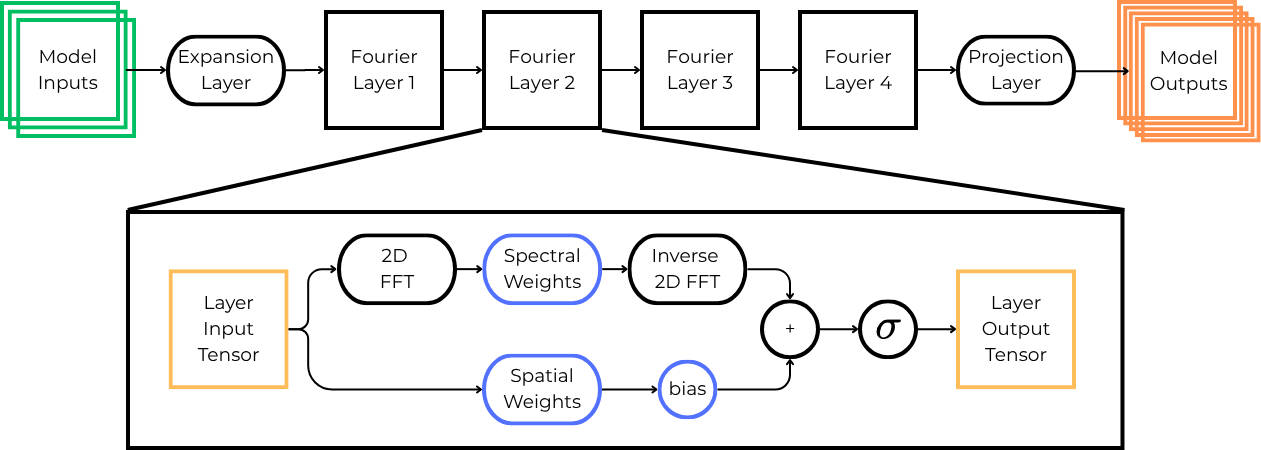
\includegraphics[width=\textwidth]{Figures/Methods/FNO_architecture.png}
\caption{The FNO model architecture used in this project. The input data is first expanded according to the hidden-channels parameter, allowing multiple latent features to be represented between Fourier layers. Each Fourier layer is shown in detail in the expanded view. The data passing through a Fourier layer is processed through two learned branches: a pointwise branch, which applies a learned linear transformation in the spatial representation, and a spectral branch, which applies a fast Fourier transform (FFT), multiplies the retained Fourier modes by learned spectral weights, and then applies an inverse FFT. The outputs of both branches, along with a learnable bias term, are summed before passing through a nonlinear activation function. After passing through four Fourier layers, the latent representation is projected from the hidden-channel dimensionality to the final output dimensions.}
\label{fig:FNO_architecture}
\end{figure}


%%%%%%%%%%%%%%%%%%%%%%%%%%%%%%%%%%%%%%%%%%%%%%%%%%%%%%%%%%%%%%%%%%%%%%
\subsection{Metamaterial Design Space}
\label{ssec:metamaterial_design_space}
To train a surrogate model capable of predicting acoustic eigenmodes, a representative design space of acoustic metamaterials must first be defined. The design space was selected to provide sufficient geometric and material complexity to demonstrate operator learning for eigenvalue PDEs while maintaining computationally tractable finite element simulations for dataset generation.

The dataset is restricted to two-dimensional acoustic metamaterials composed of infinitely repeating square unit cells exhibiting eight-fold symmetry. Each unit cell is discretized onto a $32\times32$ spatial grid and represented by three material-property channels corresponding to the normalized elastic modulus, density, and Poisson's ratio. Material properties are normalized to the interval $[0,1]$ to improve numerical conditioning during training, while the corresponding physical values are recovered using the fixed material constants listed in Table \ref{tab:parameter_ranges}. The two constituent materials were chosen to represent a stiff steel alloy and a compliant polymer.

\begin{table}[h]
  \centering
  \begin{tabular}{|c|c|c|c|c|c|c|}
    \hline
    $\text{Parameter}$ & $E_{\text{polymer}}$ & $E_{\text{steel}}$ & $\rho_{\text{polymer}}$ & $\rho_{\text{steel}}$ & $\nu_{\text{polymer}}$ & $\nu_{\text{steel}}$ \\
    \hline
    $\text{Units}$ & $\text{Pa}$ & $\text{Pa}$ & $\text{kg/m}^3$ & $\text{kg/m}^3$ & -- & -- \\
    \hline
    $\text{Value}$ & $1 \times 10^6$ & $2 \times 10^{9}$ & $1200$ & $8000$ & $0.45$ & $0.3$ \\
    \hline
  \end{tabular}
  \caption{Ranges for material parameters. The hard material is chosen to be a common steel alloy and the soft material a rubbery polymer.}
  \label{tab:parameter_ranges}
\end{table}

Unit-cell geometries are synthesized by sampling a Gaussian process with a periodic covariance kernel and subsequently enforcing eight-fold symmetry. This procedure produces smoothly varying spatial material distributions while ensuring compatibility with periodically tiled square lattices. The sampled field assumes values between $0$ and $1$, where $0$ represents pure polymer, $1$ represents pure steel, and intermediate values denote an effective mixture of the two materials below the spatial resolution of the discretization.

To investigate the influence of geometry representation on model performance, two classes of unit cells were generated. The first consists of the continuous-valued Gaussian process realizations described above and is referred to as the \emph{continuous geometry} dataset. The second is obtained by thresholding the Gaussian process samples to binary numbers, producing geometries composed exclusively of polymer and steel. This second collection is referred to as the \emph{discrete geometry} dataset. Each representation comprises approximately one-half of the total dataset.

\begin{figure}[H]
  \centering
  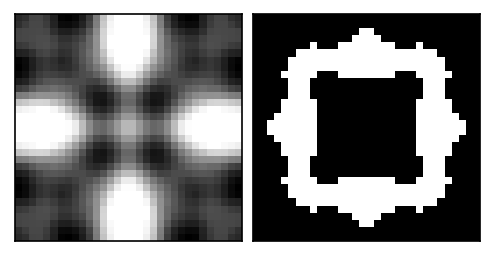
\includegraphics[width=0.5\textwidth]{Figures/Methods/continuous_and_binary_geometry_example.png}
  \caption{Example of a continuous geometry (left) and a discrete geometry (right) generated using the above process and parameters.}
  \label{fig:example_geometries}
\end{figure}

%%%%%%%%%%%%%%%%%%%%%%%%%%%%%%%%%%%%%%%%%%%%%%%%%%%%%%%%%%%%%%%%%%%%%%
\subsection{Wave Propagation Simulations} 
\label{ssec:wave_propagration_simulations}

For each metamaterial geometry, wave propagation is simulated by solving the frequency-domain linear elastodynamic equation using the finite element analysis (FEA). After spatial discretization, the governing PDE takes the generalized eigenvalue form
\begin{equation}
\label{eqn:wave_fuction}
\left( \mathbf{K}(\mathbf{k}) - \omega^2 \mathbf{M}(\mathbf{k}) \right) \mathbf{u} = \mathbf{0},
\end{equation}
where $\mathbf{K}(\mathbf{k})$ and $\mathbf{M}(\mathbf{k})$ are the stiffness and mass matrices, respectively, parameterized by the irreducible Brillouin zone (IBZ) wavevector $\mathbf{k}$, $\omega$ is the angular eigenfrequency, and $\mathbf{u}$ is the corresponding eigenvector describing the displacement field.

% Our FEA solver is implemented in the MATLAB. In the data-generation code, Eq.~\eqref{eqn:wave_fuction} is solved using intermediate steps involving five sparse matrices. The global stiffness and mass matrices, $\mathbf{K}^{\mathrm{FE}}$ and $\mathbf{M}^{\mathrm{FE}}$, are assembled once per unit-cell geometry from bilinear quadrilateral plane-stress elements and depend only on the spatial distribution of elastic moduli, density, and Poisson ratio; they do not depend on $\mathbf{k}$. Bloch periodicity at a given wavevector is enforced by a transformation matrix $\mathbf{T}(\mathbf{k})$ that relates the full mesh displacements to a smaller independent set of degrees of freedom through phase factors $\exp(i\mathbf{k}\cdot\mathbf{R})$ across opposite faces of the unit cell, where $\mathbf{R}$ is the relevant lattice translation vector. The stiffness and mass matrices appearing in Eq.~\eqref{eqn:wave_fuction} are then formed as
% \begin{equation}
% \mathbf{K}(\mathbf{k}) = \mathbf{T}(\mathbf{k})^{\dagger}\mathbf{K}^{\mathrm{FE}}\,\mathbf{T}(\mathbf{k}),
% \qquad
% \mathbf{M}(\mathbf{k}) = \mathbf{T}(\mathbf{k})^{\dagger}\mathbf{M}^{\mathrm{FE}}\,\mathbf{T}(\mathbf{k}),
% \end{equation}
% where $\dagger$ indicates the Hermitian transpose. These matrices are used directly in the eigenvalue solve.

The IBZ is discretized into $25$ $x$ wave numbers and $13$ $y$ wave numbers, totaling $25 \times 13 = 325$ unique wavevectors covering the IBZ half plane. For each wavevector, the six lowest eigenfrequencies (bands) were computed using a custom finite element analysis (FEA) MATLAB script (see section \ref{sec:Repository} for implementation details). 

Each eigenvector $\mathbf{u}$ consists of two complex-valued displacement fields, $(u_x,u_y)$, which are separated into their real and imaginary components to produce four real-valued output channels, $(u_{x,real},u_{x,imag},u_{y,real},u_{y,imag})$. The corresponding eigenfrequency $\omega$ is encoded as a spatially uniform fifth channel, resulting in a target tensor of size $5\times32\times32$. Combined with the three-channel material representation described in the previous subsection, each simulation therefore produces a supervised learning sample mapping
\begin{equation*}
\mathbb{R}^{3\times32\times32}
\rightarrow
\mathbb{R}^{5\times32\times32}.
\end{equation*}
The overall finite element data-generation procedure is summarized in Figure \ref{fig:FEA_full_process}.

\begin{figure}[H]
  \centering
  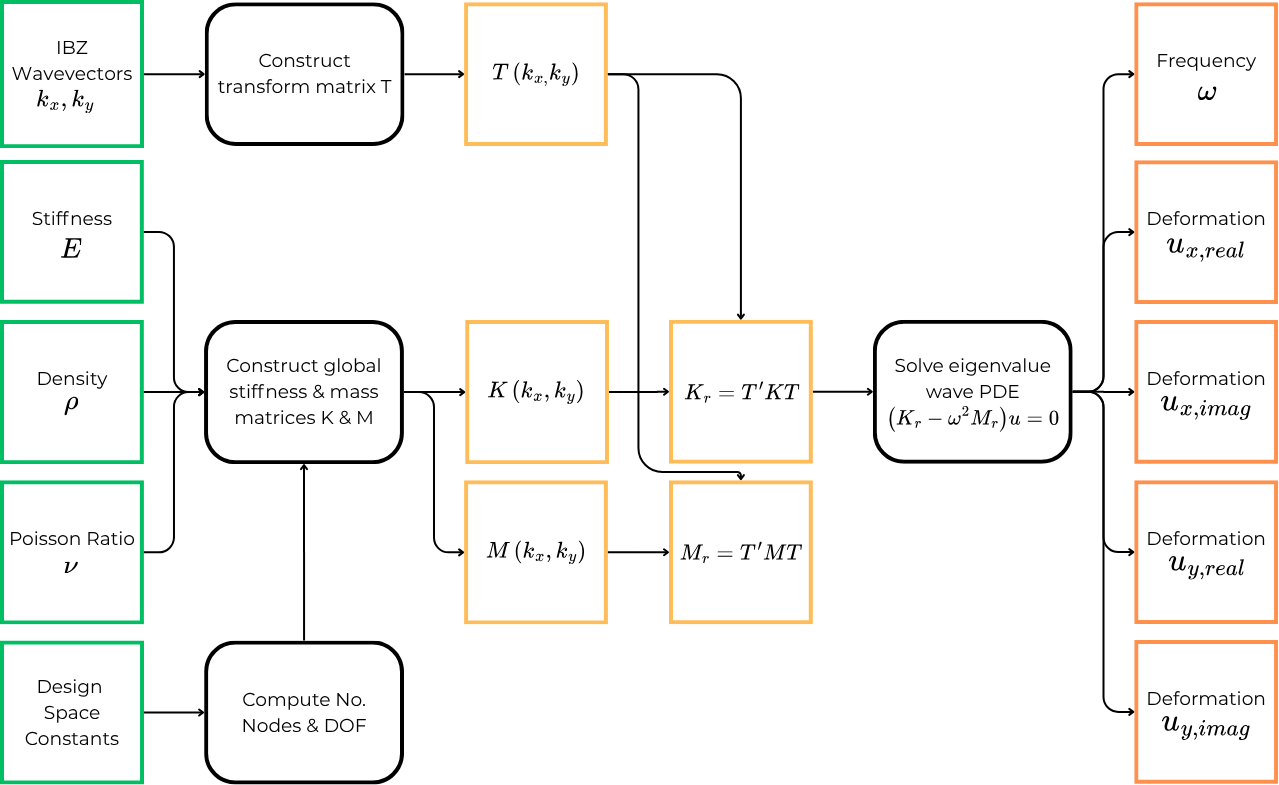
\includegraphics[width=\textwidth]{Figures/Methods/distilled_FEA_process.png}
  \caption{Flowchart of the FEA data generation method. Green squares represent varying inputs to the process, and orange squares represent computed quantities of the FEA process. Black rounded rectangles represent subroutines of the FEA process. The process starts with inputs of defined densities, stiffnesses, and Poisson ratios for each pixel of a metamaterial unit cell geometry (each a $32 \times 32$ pixel grid of values ranging from 0 to 1), along with a chosen $k_x$ and $k_y$ wavevector representing the stimulus to the metamaterial. A custom optimized FEA solver takes these inputs and produces intermediate transformation matrices, and then uses those to solve an eigenvalue matrix problem to produce the solution displacement fields (eigenvectors) and frequency $\omega$ (eigenvalues) for the given inputs.}
  \label{fig:FEA_full_process}
\end{figure}

%%%%%%%%%%%%%%%%%%%%%%%%%%%%%%%%%%%%%%%%%%%%%%%%%%%%%%%%%%%%%%%%%%%%%%
\subsection{Input Wavelet Encoding}
\label{ssec:input_wavelet_encoding}
To allow the FNO model to toggle between PDE solutions for a given geometry, information must be fed to the model indicating which excitation waveform (wavevectors) and deformation mode (band) we are looking for a solution to. This information is given in the form of a wavevector embedding, which we have found to yield superior results compared with a constant field embedding (2D matrices of the same value) or a sinusoidal embedding (2D sinusoidal fields with constants encoded as the sinusoidal frequency). A discussion on why wavelet encodings are superior is found in the results \todo{add section reference here} presented later in this paper.

For the wavelet encodings, we use a 1D Gabor wavelet transform to map band numbers to unique wavelet images (see Algorithm \ref{alg:1d_gabor_embedding}), and a 2D Gabor wavelet transform to map x and y wavevectors to another set of unique wavelet images (see Algorithm \ref{alg:2d_gabor_embedding}). These representations show rich variation both in the spatial domain and in the Fourier domain, which allows for FNO model weights of both branches to richly interact with the wavelet representation, leading to better learning outcomes. 

\begin{figure}[H]
    \centering
    \begin{subfigure}{\textwidth}
        \centering
        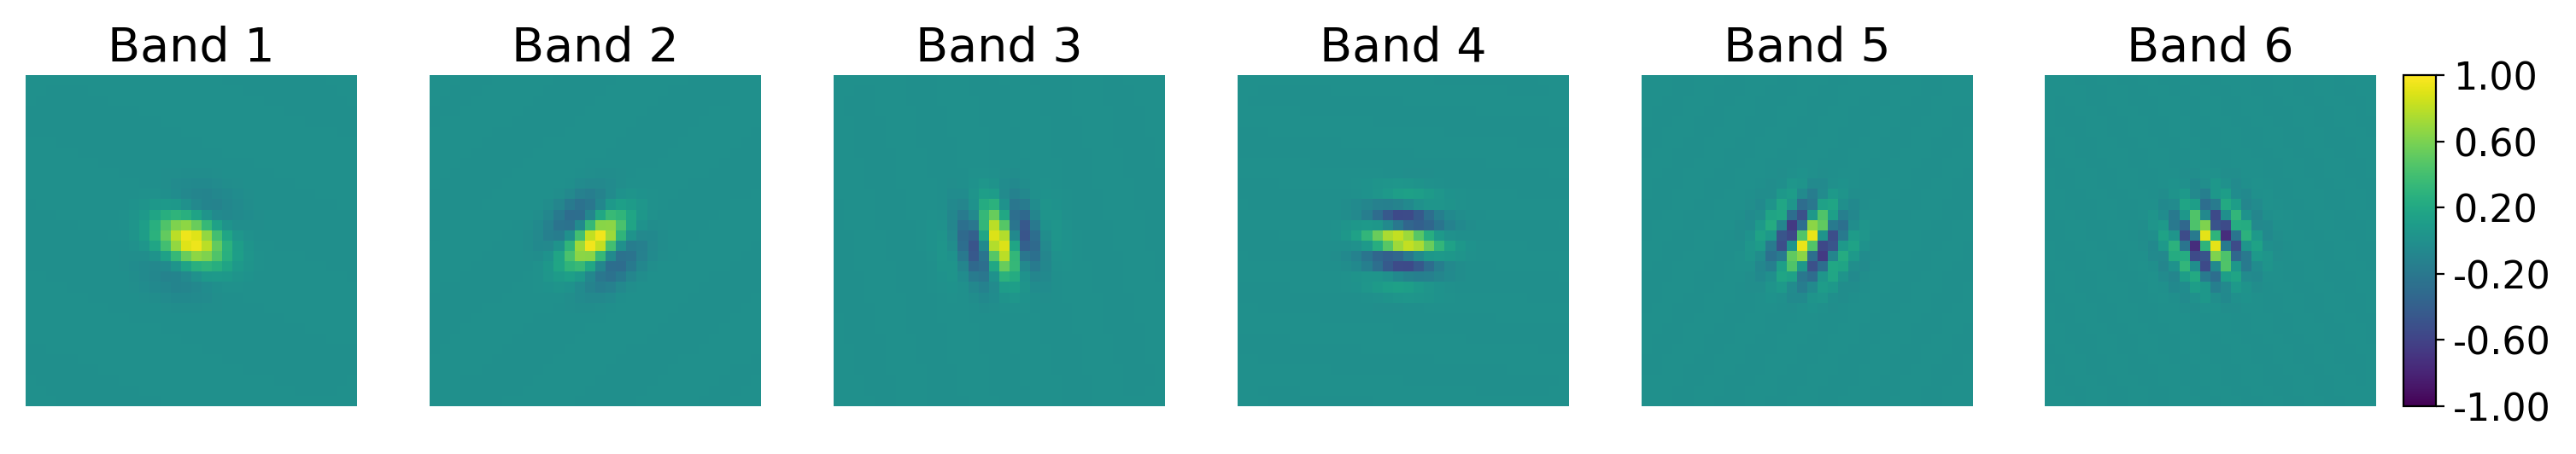
\includegraphics[width=\textwidth]{Figures/Methods/1D wavelet encoding.png}
        \caption{The wavelet spatial encoding for band integer.}
        \label{fig:1D_wavelet_encoding_spatial}
    \end{subfigure}  
    \begin{subfigure}{\textwidth}
        \centering
        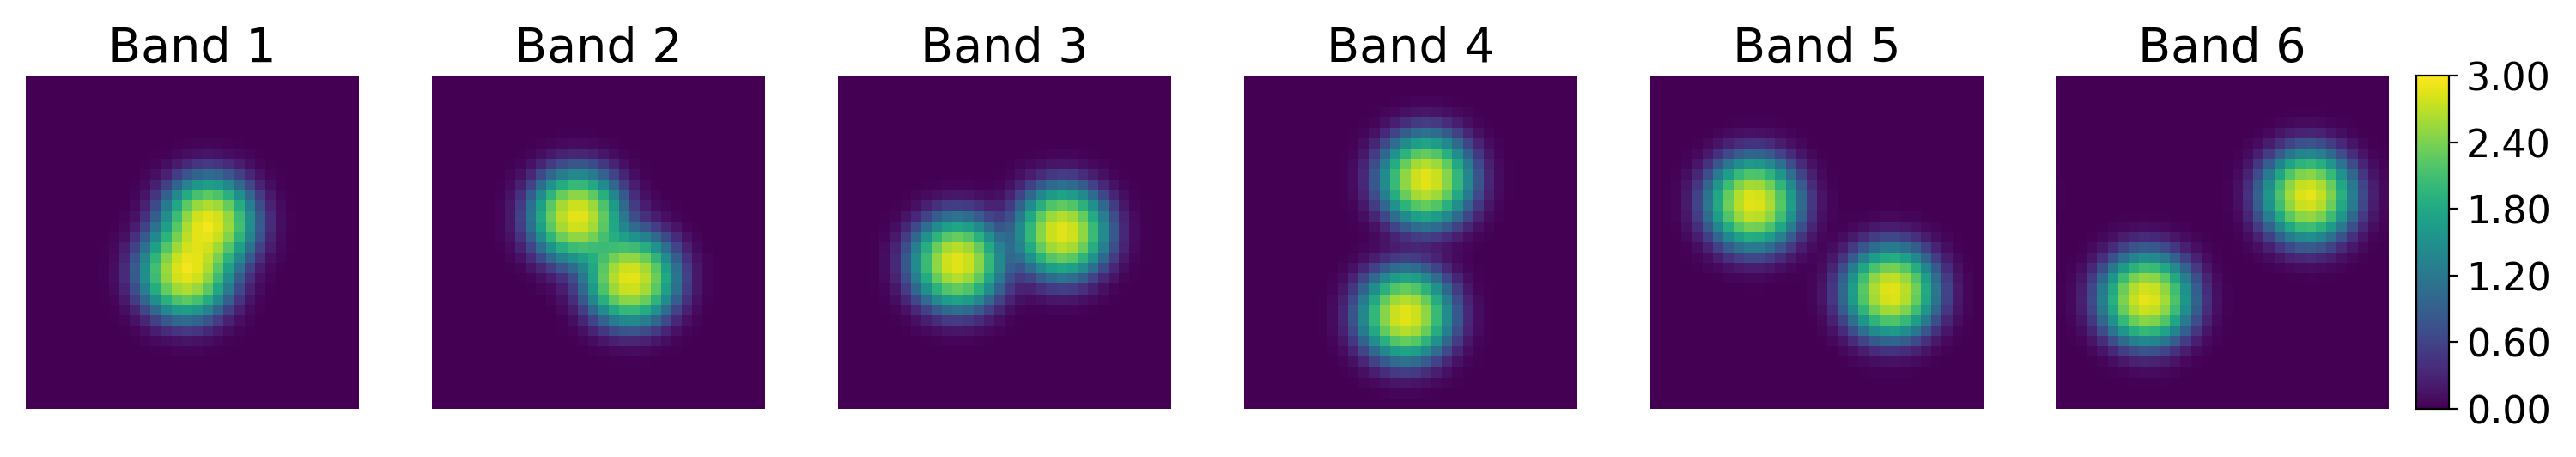
\includegraphics[width=\textwidth]{Figures/Methods/1D wavelet encoding fft.png}
        \caption{The FFT of the above wavelet spatial encodings.}
        \label{fig:1D_wavelet_encoding_fft}
    \end{subfigure}
    \caption{The wavelet encoding of the band integer (fig. \ref{fig:1D_wavelet_encoding_spatial}) and its FFT (fig. \ref{fig:1D_wavelet_encoding_fft}). Each band corresponds to a unique wavelet with representation in both spatial and spectral domains.}
    \label{fig:1D_wavelet_encoding}
\end{figure}

\begin{figure}[H]
    \centering
    \begin{subfigure}{\textwidth}
        \centering
        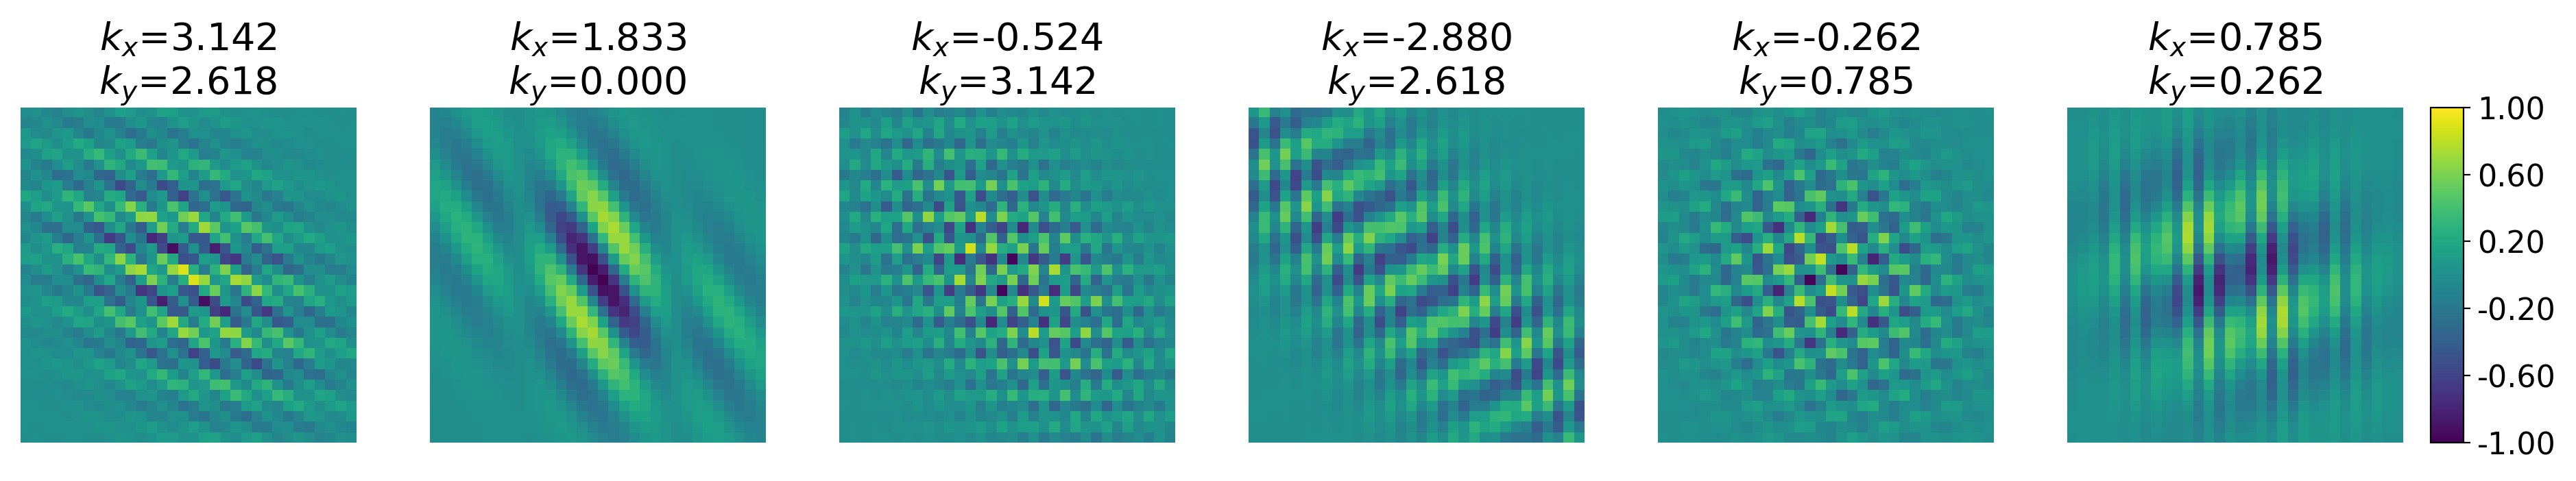
\includegraphics[width=\textwidth]{Figures/Methods/2D wavelet encoding.png}
        \caption{The wavelet spatial encoding for $x$ and $y$ wavevectors.}
        \label{fig:2D_wavelet_encoding_spatial}
    \end{subfigure}  
    \begin{subfigure}{\textwidth}
        \centering
        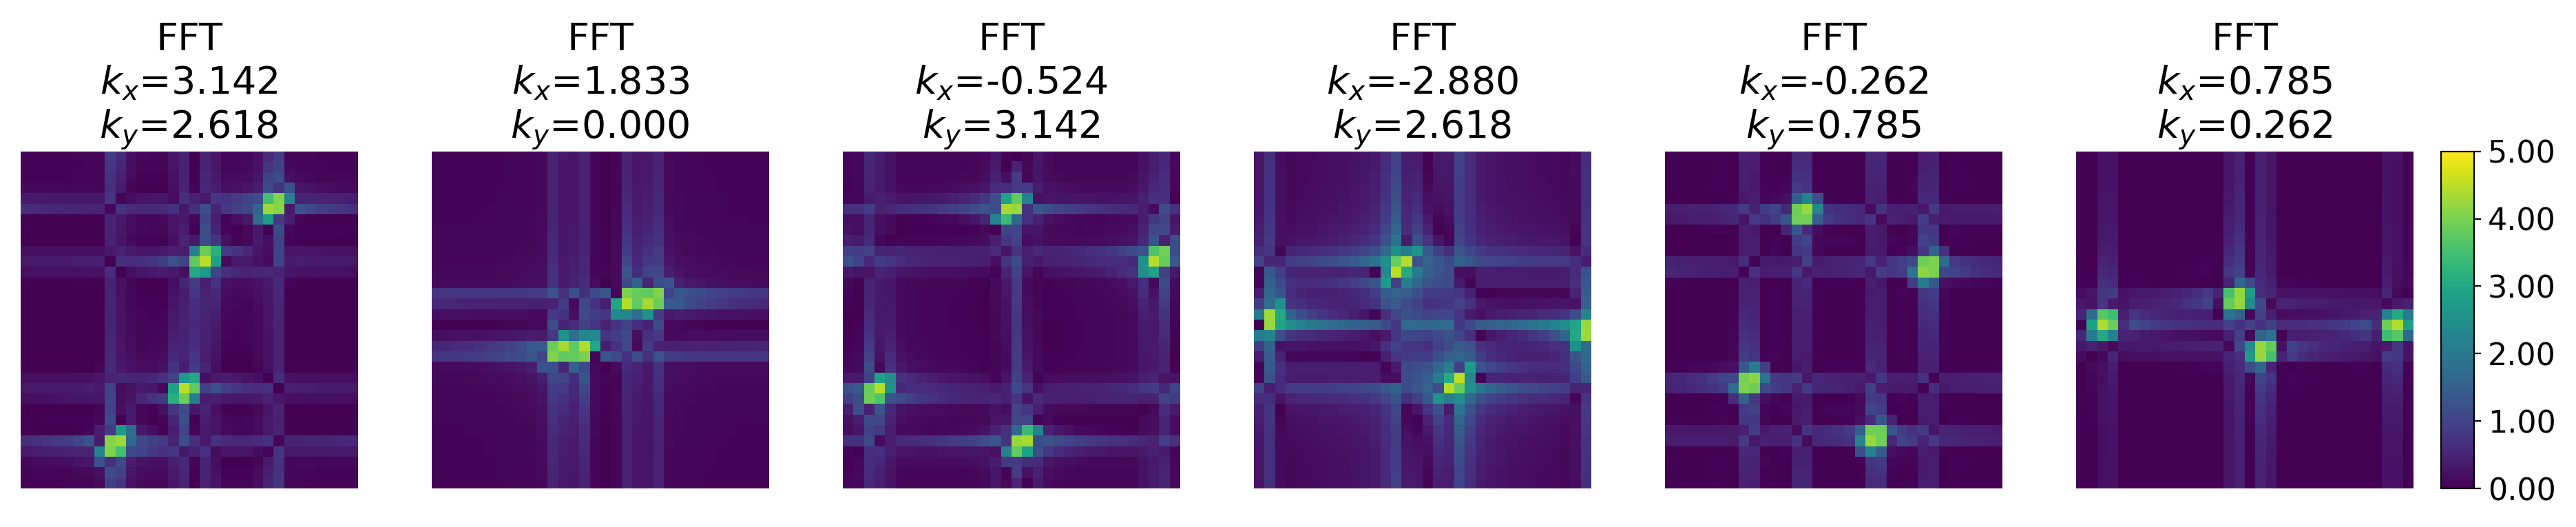
\includegraphics[width=\textwidth]{Figures/Methods/2D wavelet encoding fft.png}
        \caption{The FFT of the above wavelet spatial encodings.}
        \label{fig:2D_wavelet_encoding_fft}
    \end{subfigure}
    \caption{The wavelet encoding of the $x$ and $y$ wavevectors (\ref{fig:2D_wavelet_encoding_spatial}) and its FFT \ref{fig:2D_wavelet_encoding_fft}. The actual wavevectors are shown in the subplot titles. For each $k_x$ and $k_y$ value pair, there is a unique mapping in both the spatial and spectral domain representations.}
    \label{fig:2D_wavelet_encoding}
\end{figure}

%%%%%%%%%%%%%%%%%%%%%%%%%%%%%%%%%%%%%%%%%%%%%%%%%%%%%%%%%%%%%%%%%%%%%%


%%%%%%%%%%%%%%%%%%%%%%%%%%%%%%%%%%%%%%%%%%%%%%%%%%%%%%%%%%%%%%%%%%%%%%
\subsection{Dataset Construction} 
\label{ssec:dataset_construction}
Our full dataset contains 24000 geometries, randomly generated as described in prior subsections. Half are discrete valued with only 0s or 1s in each pixel location representing one of the two materials, while the other half are continuous valued with any value between 0 and 1 inclusive at each pixel location, representing blended materials at each pixel location. Each geometry has 6 possible bands each with 325 possible wavevectors (representing a mesh grid the IBZ half plane) per band, resulting in $24000 \times 6 \times 325 = 46,800,000$ sample pairs of inputs with shape $(3 \times 32 \times 32)$ and outputs of shape $(5 \times 32 \times 32)$. The data is stored with float16 datatype format in PyTorch tensors. 

% Due to computational and memory constraints, for each of the 9600 geometries, a random 1/4 of the 325 waveforms and 1/2 of the 6 deformation modes (i.e., 3 bands) were retained for FNO training. This stochastic downsampling maintains a diverse sampling of wave-structure interactions while reducing the size of the training dataset by a factor of 8.

\begin{figure}[H]
  \centering
  \begin{subfigure}[c]{0.5\textwidth}
    \centering
    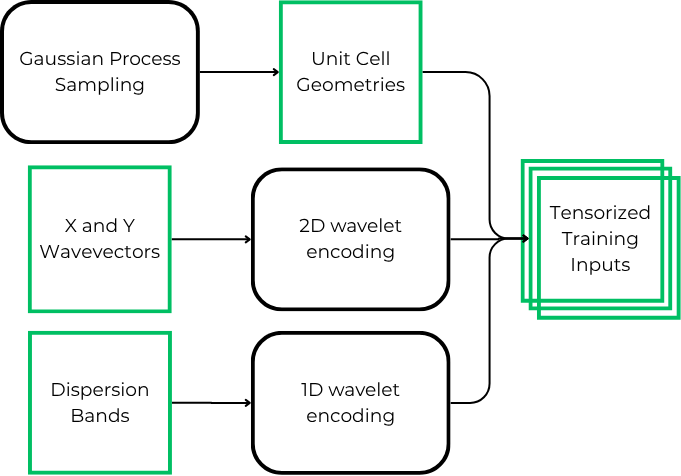
\includegraphics[scale=0.35]{Figures/Methods/distilled_input_tensorization.png}
    %
\includegraphics{Figures/distilled_input_tensorization.png}
    \caption{Construction of the input tensors}
    \label{fig:input_dataset_construction}
  \end{subfigure}%
  \hfill
  \begin{subfigure}[c]{0.5\textwidth}
    \centering
    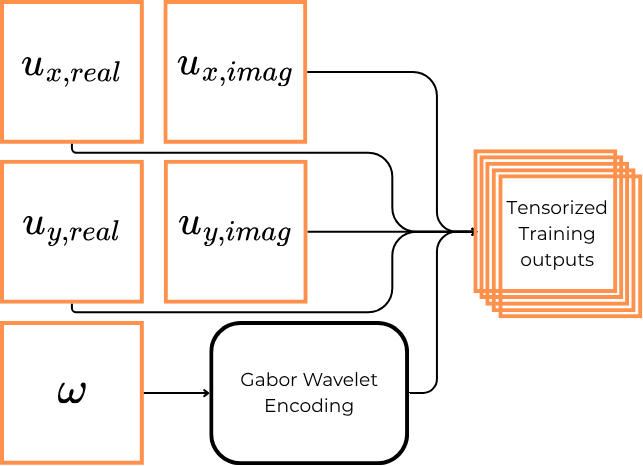
\includegraphics[scale=0.35]{Figures/Methods/distilled_output_tensorization2.png}
    %
\includegraphics{Figures/distilled_outout_tensorization.png}
    \caption{Construction of the output tensors}
    \label{fig:output_dataset_construction}
  \end{subfigure}
  \caption{Subfigure \subref{fig:input_dataset_construction} and \subref{fig:output_dataset_construction} shows the process of input data from subsection \ref{ssec:metamaterial_design_space} and output data from subsection \ref{ssec:wave_propagration_simulations} being tensorized for ingestion to the FNO model respectively. Note the wavelet embedding steps on fundamentally scalar quantities.}
  \label{fig:dataset_construction}
\end{figure}

%%%%%%%%%%%%%%%%%%%%%%%%%%%%%%%%%%%%%%%%%%%%%%%%%%%%%%%%%%%%%%%%%%%%%%


\subsection{Training Procedure}
\label{ssec:training_procedure}
The Fourier Neural Operator was trained using supervised learning on paired inputs and outputs described in Section \ref{sec:Methodology}. Each training sample consists of a $3 \times 32 \times 32$ input tensor (geometry and wavelet embeddings) and a $5 \times 32 \times 32$ output tensor (displacement field components and eigenfrequency).

6 loss functions were trialed as performance evaluation criterion: mean absolute error (MAE), mean squared error (MSE), normalized MAE, normalized MSE, Huber (smooth L1), and structural similarity index (SSI). Losses were evaluated and aggregated across all 5 output channels. The best performing loss criterion is the Huber loss and is shown below. Details on the other loss functions trialed can be found in Supplemental Information.
% \begin{equation*}
%     \mathcal{L}_{\text{MAE}} = \frac{1}{HW} \sum_{i=0}^{H-1} \sum_{j=0}^{W-1} \sum_{c=0}^{4} \left| \hat{u}_{c}(i,j) - u_{c}(i,j) \right|
% \end{equation*}

% \begin{equation*}
%     \mathcal{L}_{\text{MSE}} = \frac{1}{HW} \sum_{i=0}^{H-1} \sum_{j=0}^{W-1} \sum_{c=0}^{4} \left( \hat{u}_{c}(i,j) - u_{c}(i,j) \right)^2
% \end{equation*}
% \begin{equation*}
%     \mathcal{L}_{\text{NMAE}} = \frac{1}{HW} \sum_{i=0}^{H-1} \sum_{j=0}^{W-1} \sum_{c=0}^{4} \frac{\displaystyle \left| \hat{u}_{c}(i,j) - u_{c}(i,j) \right|}{\left| u_{c}(i,j) \right| + \varepsilon}
% \end{equation*}
% \begin{equation*}
%     \mathcal{L}_{\text{NMSE}} = \frac{1}{HW} \sum_{i=0}^{H-1} \sum_{j=0}^{W-1} \sum_{c=0}^{4} \frac{\displaystyle \left(\hat{u}_{c}(i,j) - u_{c}(i,j) \right)^2}{\left( u_{c}(i,j) \right)^2 + \varepsilon}
% \end{equation*}
% \begin{equation*}
% \mathcal{L}_{\text{Huber}} = 
% \begin{cases}
% \mathcal{L}_{\text{MAE}}, & \mathcal{L}_{\text{Huber}} \ge 10^{-3}, \\
% \mathcal{L}_{\text{MSE}}, & \mathcal{L}_{\text{Huber}} < 10^{-3}.
% \end{cases}
% \end{equation*}

\begin{equation*}
\mathcal{L}_{\text{Huber}}
=
\frac{1}{HW}
\sum_{i=0}^{H-1}
\sum_{j=0}^{W-1}
\sum_{c=0}^{4}
\begin{cases}
\dfrac{1}{2}\left(\hat{u}_c(i,j)-u_c(i,j)\right)^2,
&
\left|\hat{u}_c(i,j)-u_c(i,j)\right|\le\delta,
\\[2ex]
\delta\left(
\left|\hat{u}_c(i,j)-u_c(i,j)\right|
-\dfrac{\delta}{2}
\right),
&
\left|\hat{u}_c(i,j)-u_c(i,j)\right|>\delta.
\end{cases}
\end{equation*}

% \begin{equation*}
% \mathcal{L}_{\text{SSIM}}
% =
% 1
% -
% \frac{1}{5}
% \sum_{c=0}^{4}
% \frac{
% \left(2\mu_{u_c}\mu_{\hat{u}_c}+C_1\right)
% \left(2\sigma_{u_c\hat{u}_c}+C_2\right)
% }{
% \left(\mu_{u_c}^2+\mu_{\hat{u}_c}^2+C_1\right)
% \left(\sigma_{u_c}^2+\sigma_{\hat{u}_c}^2+C_2\right) 
% }, \quad \text{where}
% \end{equation*}
% \begin{equation*}
% \mu_{u_c}
% =
% \frac{1}{HW}
% \sum_{i=0}^{H-1}
% \sum_{j=0}^{W-1}
% u_c(i,j), \quad 
% \sigma_{u_c\hat{u}_c}
% =
% \frac{1}{HW}
% \sum_{i=0}^{H-1}
% \sum_{j=0}^{W-1}
% \left(u_c(i,j)-\mu_{u_c}\right)
% \left(\hat{u}_c(i,j)-\mu_{\hat{u}_c}\right)
% \end{equation*}

where $H = W = 32$ (pixels) and $c \in \{0,1,2,3,4\}$ corresponds to the 5 output channels: eigenfrequency, followed by real and imaginary components of x and y displacements.

For training the FNO model, combinations of model layers, hidden channels, activation function, loss function, optimizer, and training hyperparameters were trialed. The ADAMW optimizer was found to achieve the best performance compared with other flavors of momentum based optimizers and SGD. The model and training hyperparameters tuned are showed in table \ref{tab:training_hyperparameters} in \ref{sec:supplement}, with the best performing combination italicized.

% Training was performed on a randomly down-selected subset of the full dataset. Each of the 9600 geometries was paired 81 waveforms (randomly sampled from the full 325) and 3 dispersion bands (randomly sampled from the full 6), resulting in reduced memory overhead and faster training convergence while maintaining diversity across samples.



The best combination for model hyperparameters was found to be 4 Fourier layers, 128 hidden channels, and GELU nonlinear activation function. At this layer count and hidden channel count, performance was asymptotic and greater amounts of either would drive the model further into the overfit region as well as add on additional training time. The best combination for trianing hyperparameters were the Huber loss, which is to use a which would was found to be 12 epochs, Different hyperparameters of FNO model tried in combinations. 4 Fourier layers, with 64 hidden channels and GELU activation function were found to be where performance started to asymptote with increasing model complexity, and so it was not worth the computational costs in training to use more layers or hidden channels. These are the final combination of model hyperparameters from which all data presented in this article is generated.

% \begin{figure}[H]
%     \centering
%     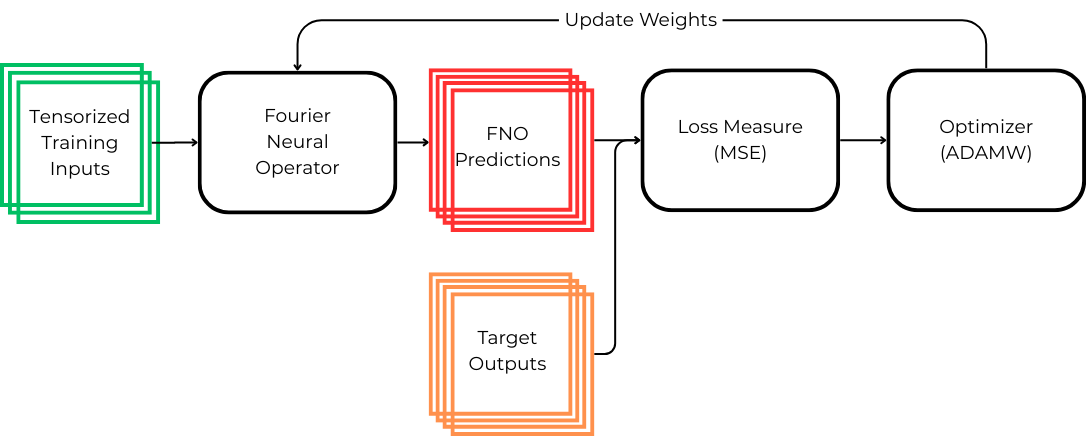
\includegraphics[scale=0.5]{Figures/Methods/model_training.png}
%     \caption{Schematic of model training loop. For compute speed and efficiency, batches of 256 inputs and outputs are run in parallel each loop.}
%     \label{fig:model_training}
% \end{figure}
% While L2 loss was used for training due to its commonality and prior successes in imaged based machine learning tasks, we chose to use L1 as the evaluation criterion for ease of interpretability of how off the model is on average for pixel predictions. Schematics of the usage of the two loss criterion in training and evaluation are shown in figure \ref{}
% \begin{figure}[H]
%     \centering
%     \begin{subfigure}[c]{0.8\textwidth}
%         \centering
%         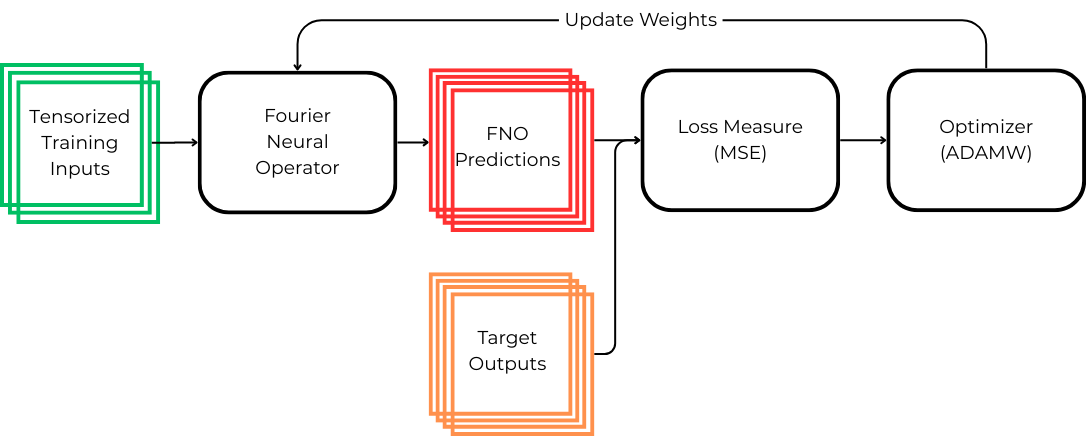
\includegraphics[scale=0.5]{Figures/Methods/model_training.png}
%         \caption{Schematic of model training loop. For compute speed and efficiency, batches of 256 inputs and outputs are run in parallel each loop.}
%         \label{fig:model_training}
%     \end{subfigure}%
%     \vspace{1em}
%     \begin{subfigure}[c]{0.8\textwidth}
%     \centering
%         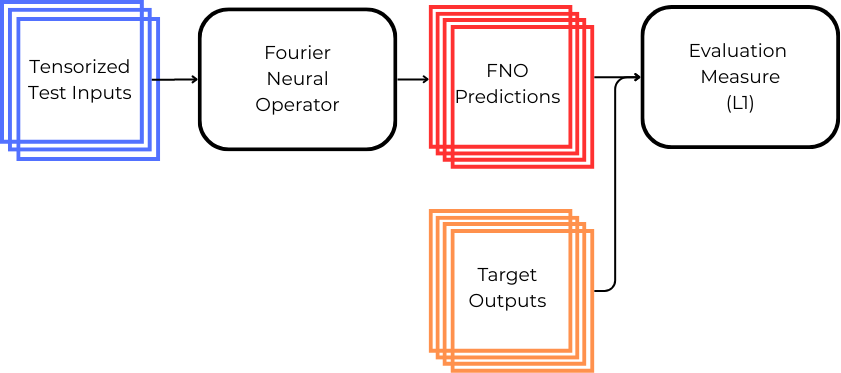
\includegraphics[scale=0.5]{Figures/Methods/model_evaluation.png}
%         \caption{Schematic of the model evaluation process. Absolute error is used here to have a simple interpretation of performance. The test datasets are of previously unseen geometries, meaning the model must be able to generalize from the highly limited number of possible geometries it is shown to the whole design space of possible geometries to do well in evaluations.}
%         \label{fig:model_evaluation}
%     \end{subfigure}
%     \caption{Subfigure \subref{fig:input_dataset_construction} and \subref{fig:output_dataset_construction} shows the training and evaluation process for the FNO model respectively.}
%     \label{fig:training_and_evaluation}
% \end{figure}

It was found that final model performance did not appreciably change for changes in step size or batch size fairly early on, so those two parameters were left fixed at 4 and 256 respectively for the remainder of the training runs. Learning rate and epochs to convergence as expected, had an inverse correlation. The higher the learning rate, the faster convergence happened, but there are two problems with high learning rates. The first is that the model may arrive at a more suboptimal combination of weights if the training rate is too high, because the movements in weight space during each backward pass remain too large to arrive close in weight space to where the loss minima would occur. The second, more interesting phenomena, is that if the learning rate is set higher than $\approx 10^{-2}$, there is instability introduced in the training, whereby at certain epochs, the loss would spike, and never come back down, usually plateauing, in all later epochs. This sort of spike is documented in other applications of ADAM family optimizers indicating the model is pushed into a region of weight space where the loss was flat for movements in any direction.

%%%%%%%%%%%%%%%%%%%%%%%%%%%%%%%%%%%%%%%%%%%%%%%%%%%%%%%%%%%%%%%%%%%%%%
\section{Results and Discussion}
This section presents the final model results in the following cases:
\begin{itemize}
    \item[\checked] Performance on displacement field prediction
    \item[\checked] Performance on eigenvalue prediction
    \item[\checked] Performance across multiple geometries
    \item[\checked] Performance variation with binary geometry discontinuity measures
    \item[\unchecked] Performance variation with encoding strategies
    \item[\unchecked] Performance variation with training hyperparameters and loss function
\end{itemize}

% In our search through the best encoding scheme for inputs, datatype representation for outputs, model architecture hyperparameters, and training hyperparameters for our FNO eigenvalue PDE solver, we discovered the following notable results.  

%%%%%%%%%%%%%%%%%%%%%%%%%%%%%%%%%%%%%%%%%%%%%%%%%%%%%%%%%%%%%%%%%%%%%%
\subsection{Displacement Field Prediction}
We next evaluate the trained Fourier Neural Operator on its predictions of the Bloch displacement fields $(u_x,u_y)$. For each unseen test sample, the prediction error is measured by the normalized mean absolute error (NMAE) over the four real-valued displacement channels, $(u_{x,\mathrm{real}},u_{x,\mathrm{imag}},u_{y,\mathrm{real}},u_{y,\mathrm{imag}})$. Ranking samples by this NMAE defines a performance distribution from which we select representative cases at the $25$th, $50$th, and $75$th percentiles, corresponding to relatively weak, median, and relatively strong predictions. The same percentile comparison is shown for both the binarized and continuous material datasets, allowing direct visual assessment of how well the model recovers the spatial structure of the displacement modes across contrasting geometry regimes.

\subsubsection{Continuous Geometries}
\begin{figure}[H]
    \centering
    \begin{subfigure}[c]{0.75\textwidth}
        \centering
        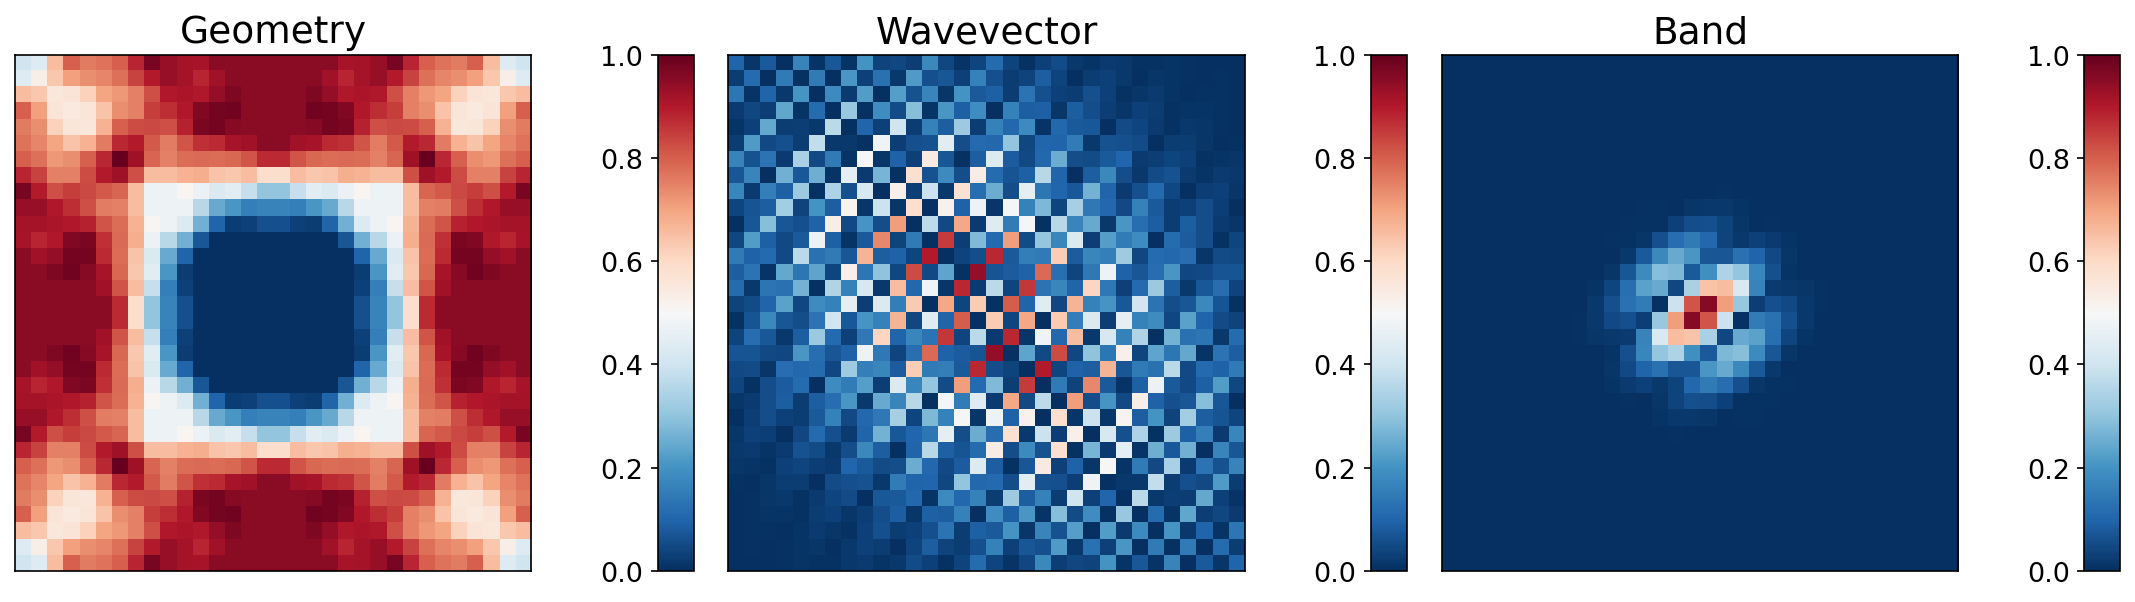
\includegraphics[width=\textwidth]{Figures/Fields C/c_test_nmae_p25_g452_w224_b1_input.png}
        \caption{Input sample at the 25th percentile of performance for unseen continuous valued geometries.}
        \label{fig:c_p25_input}
    \end{subfigure}
    \vspace{1em}
    \begin{subfigure}[c]{\textwidth}
    \centering
        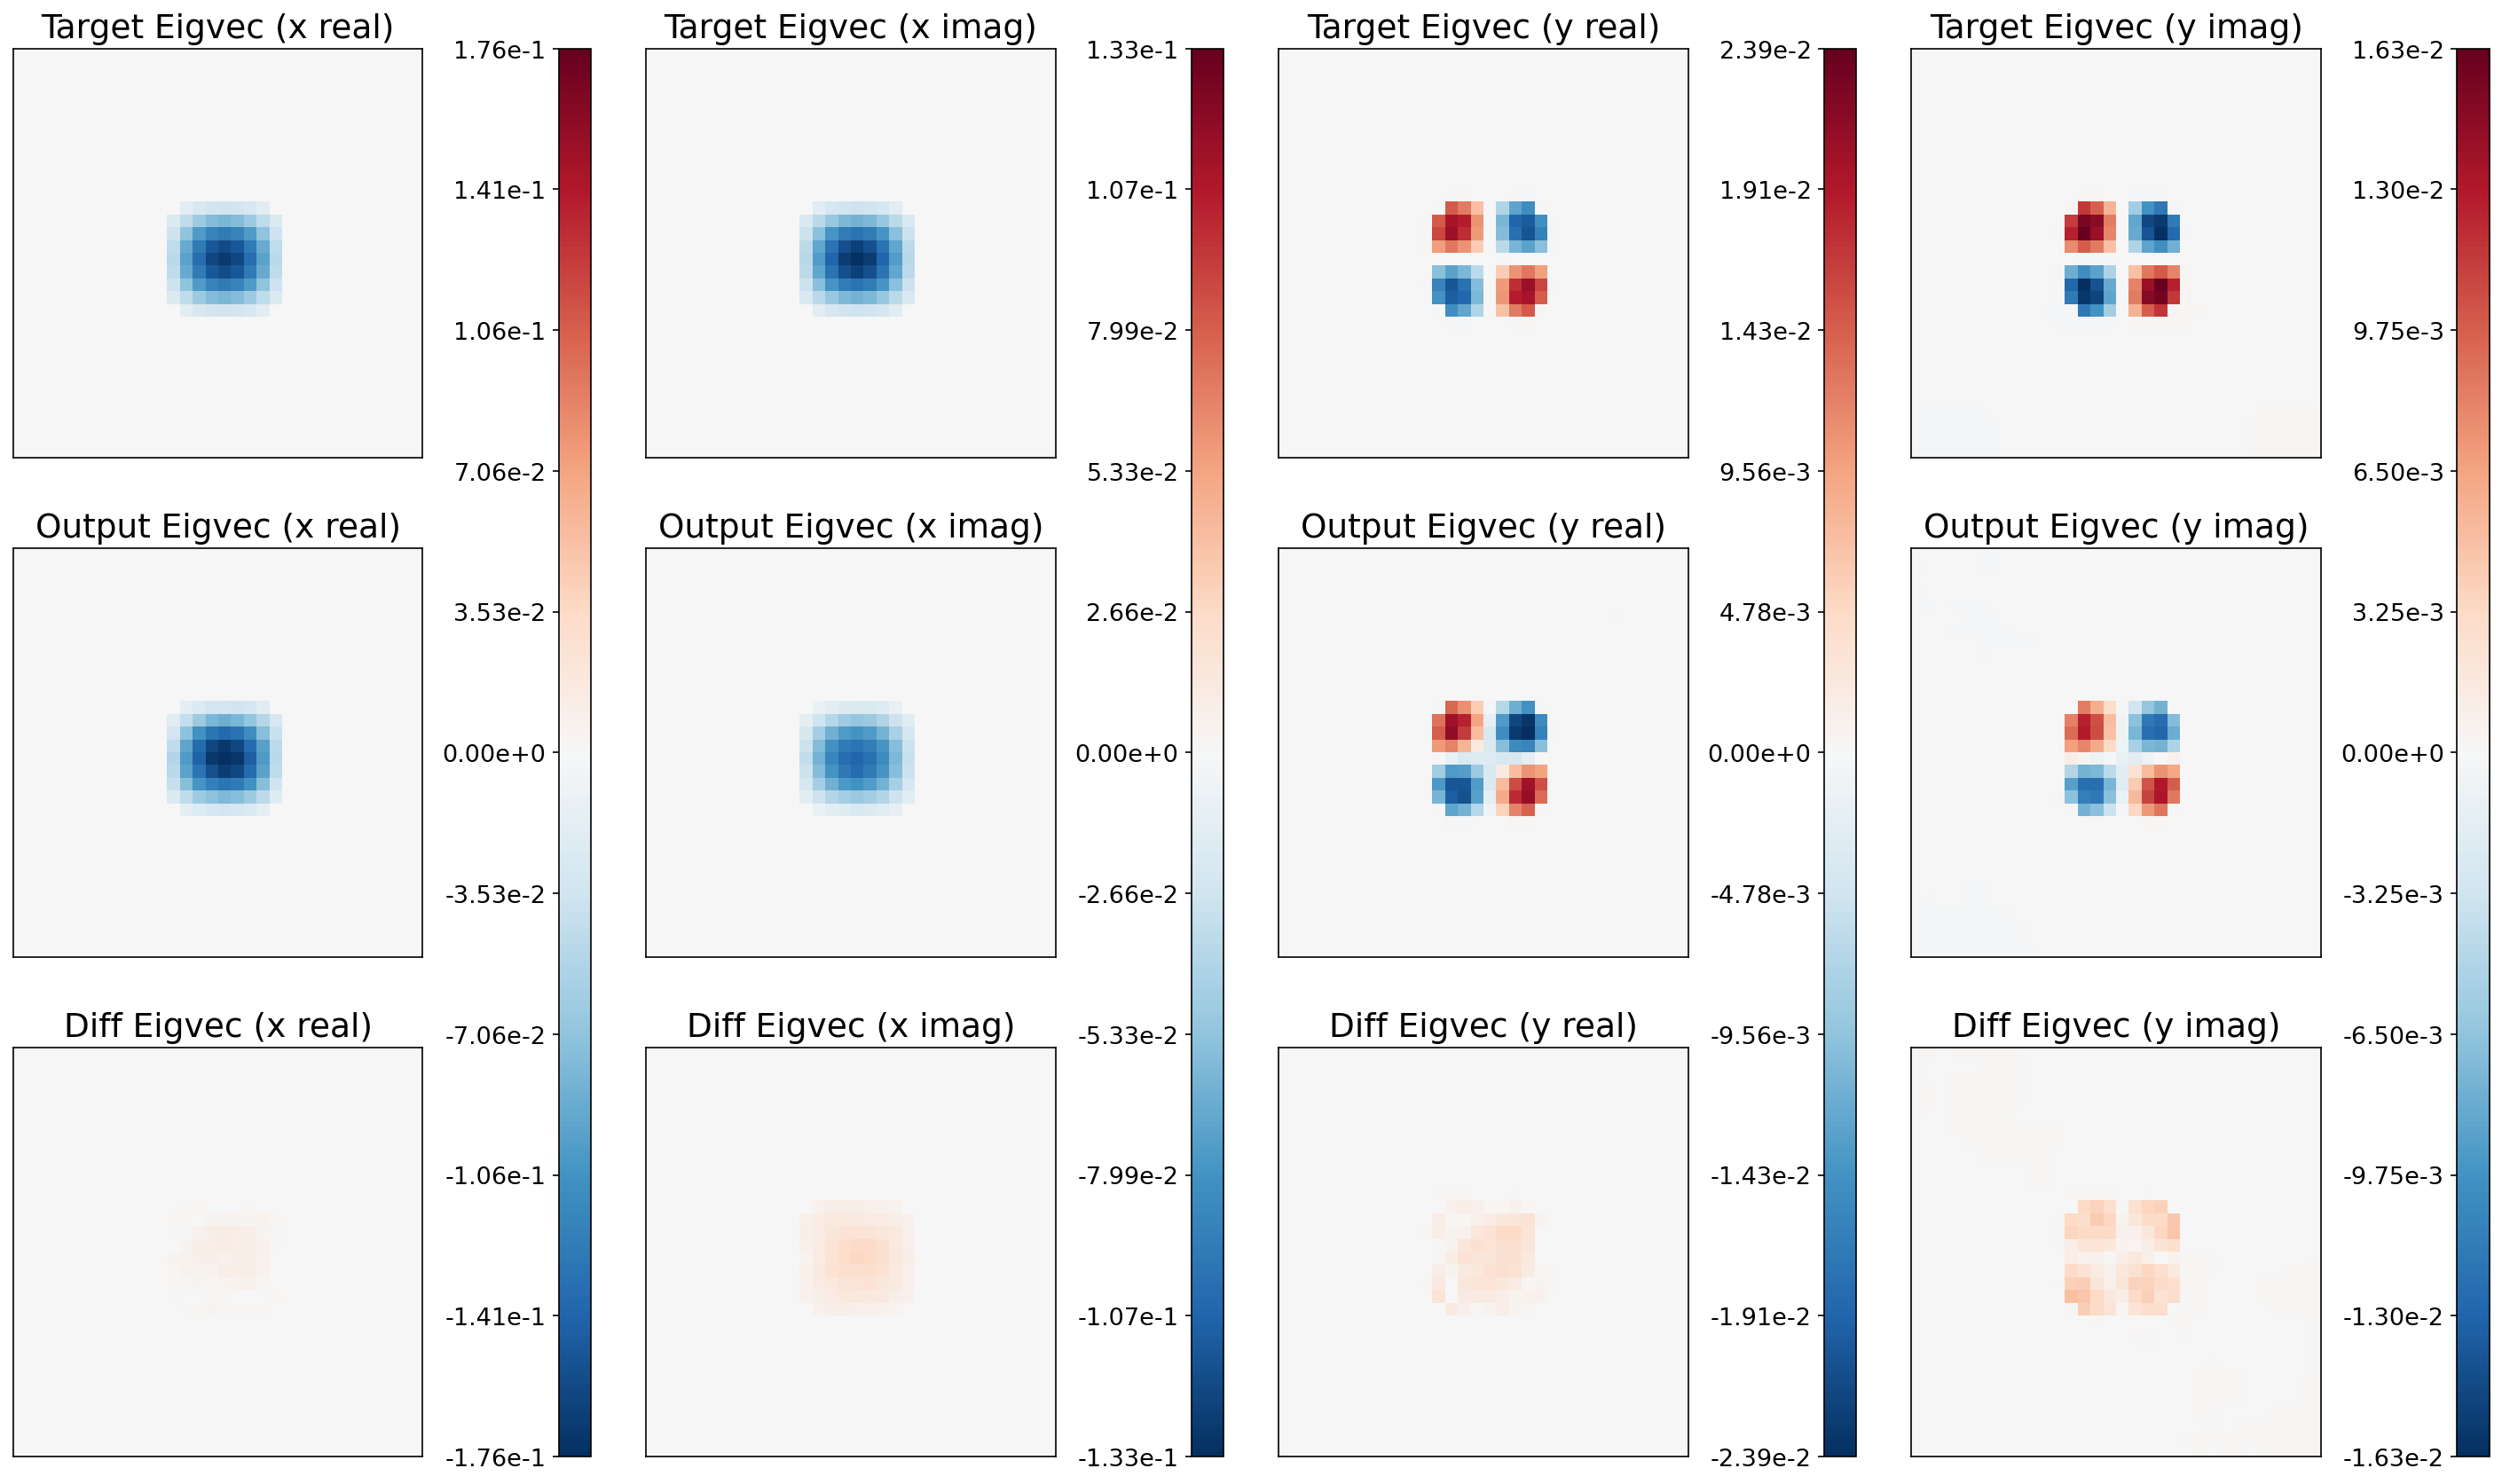
\includegraphics[width=\textwidth]{Figures/Fields C/c_test_nmae_p25_g452_w224_b1_fields.png}
        \caption{Output predictions at the 25th percentile of performance for unseen continuous valued geometries. The first row are target fields, followed by prediction fields on the second row, and difference fields on the third. At the 25th percentile, prediction outcomes are already fairly good, with accurate representations of scale and structure.}
        \label{fig:c_p25_output}
    \end{subfigure}
\end{figure}

\begin{figure}[H]
    \centering
    \begin{subfigure}[c]{0.75\textwidth}
        \centering
        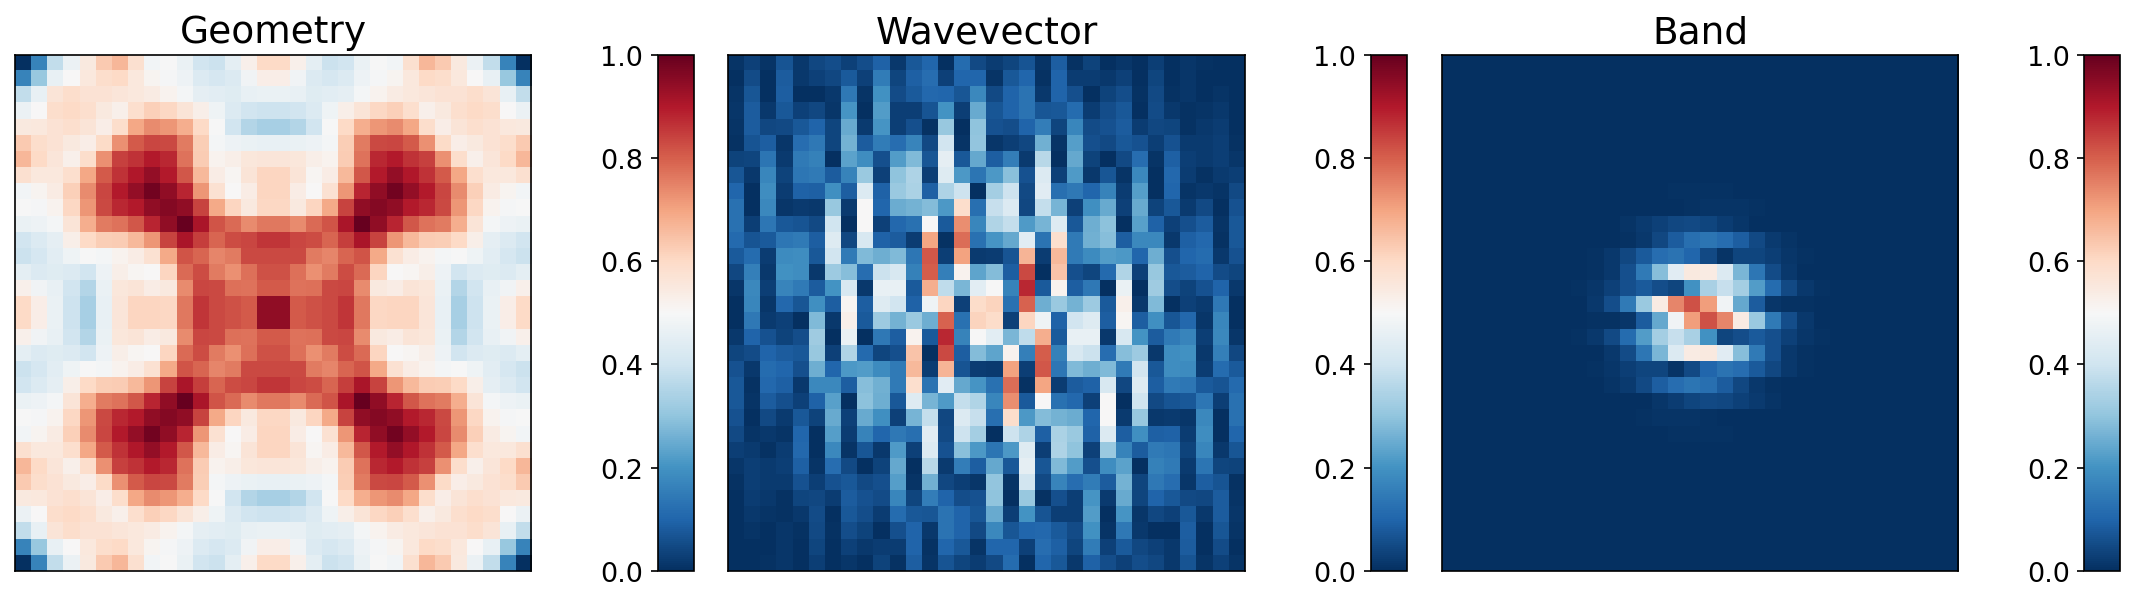
\includegraphics[width=\textwidth]{Figures/Fields C/c_test_nmae_p50_g183_w41_b3_input.png}
        \caption{Input sample at the 50th percentile of performance for unseen continuous valued geometries.}
        \label{fig:c_p50_input}
    \end{subfigure}
    \vspace{1em}
    \begin{subfigure}[c]{\textwidth}
    \centering
        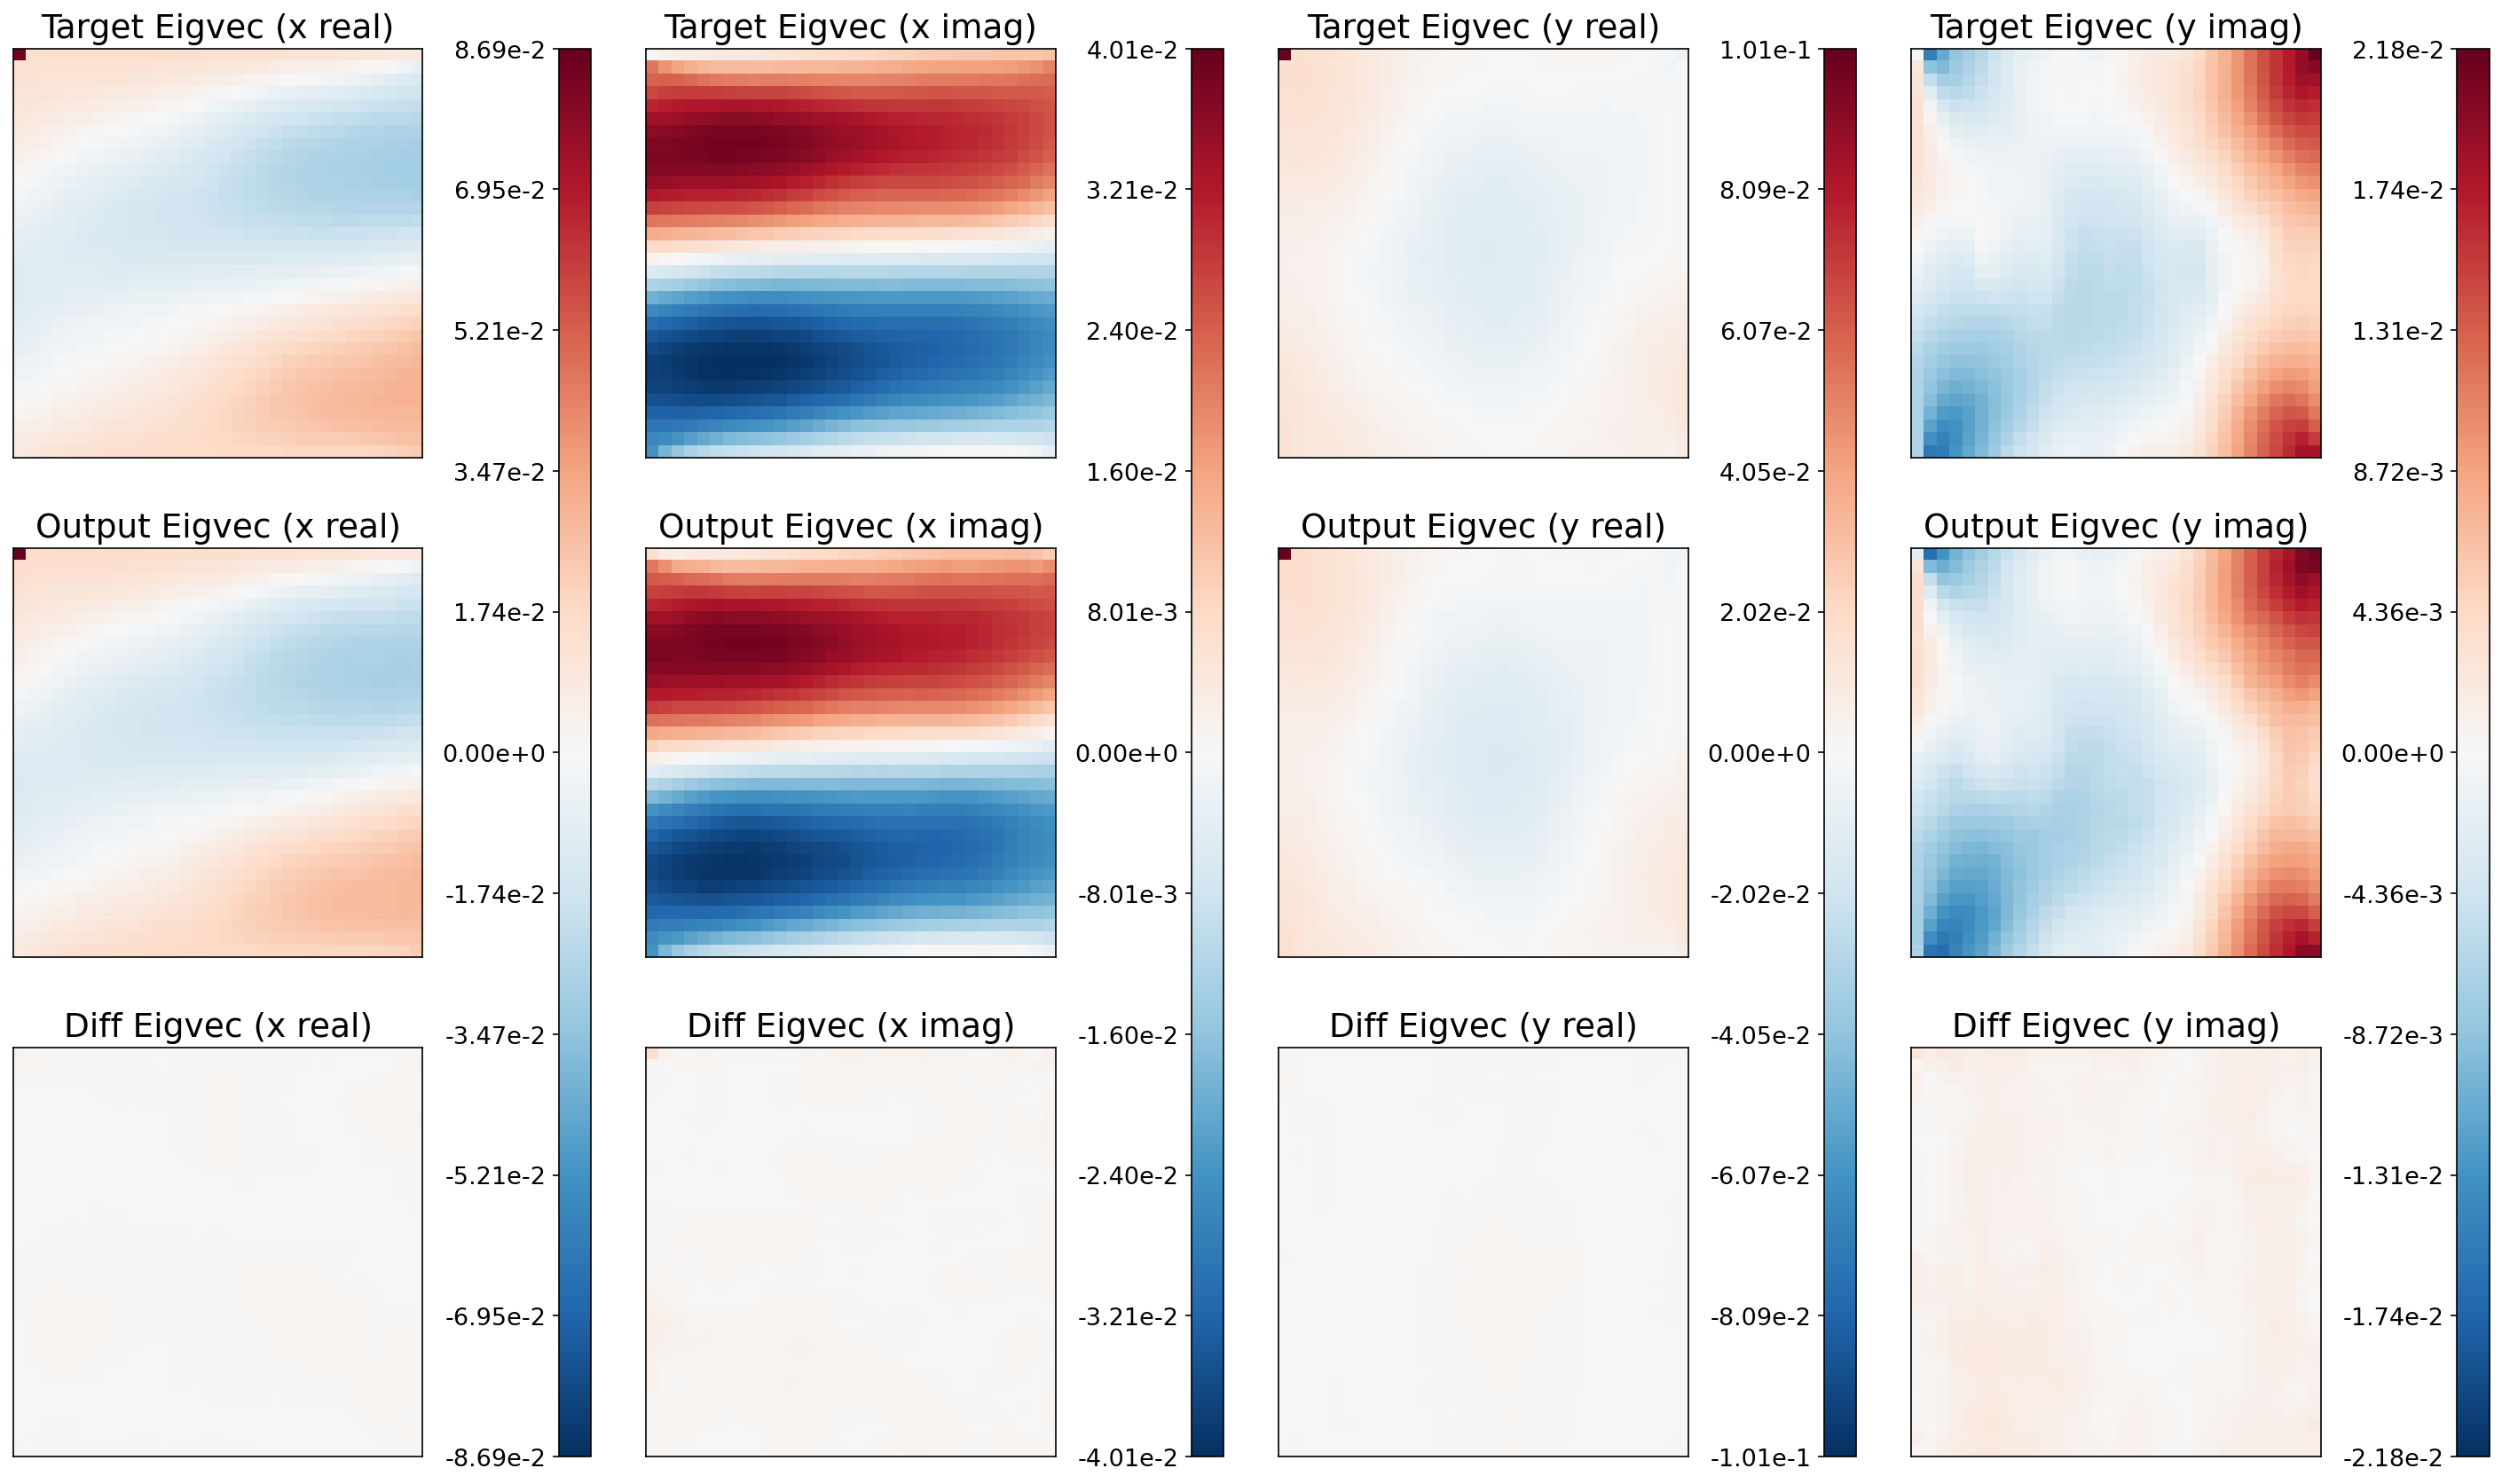
\includegraphics[width=\textwidth]{Figures/Fields C/c_test_nmae_p50_g183_w41_b3_fields.png}
        \caption{Output predictions at the 50th percentile of performance for unseen continuous valued geometries. The first row are target fields, followed by prediction fields on the second row, and difference fields on the third. Predictions are able to consistently capture complex structures without graininess.}
        \label{fig:c_p50_output}
    \end{subfigure}
\end{figure}

\begin{figure}[H]
    \centering
    \begin{subfigure}[c]{0.75\textwidth}
        \centering
        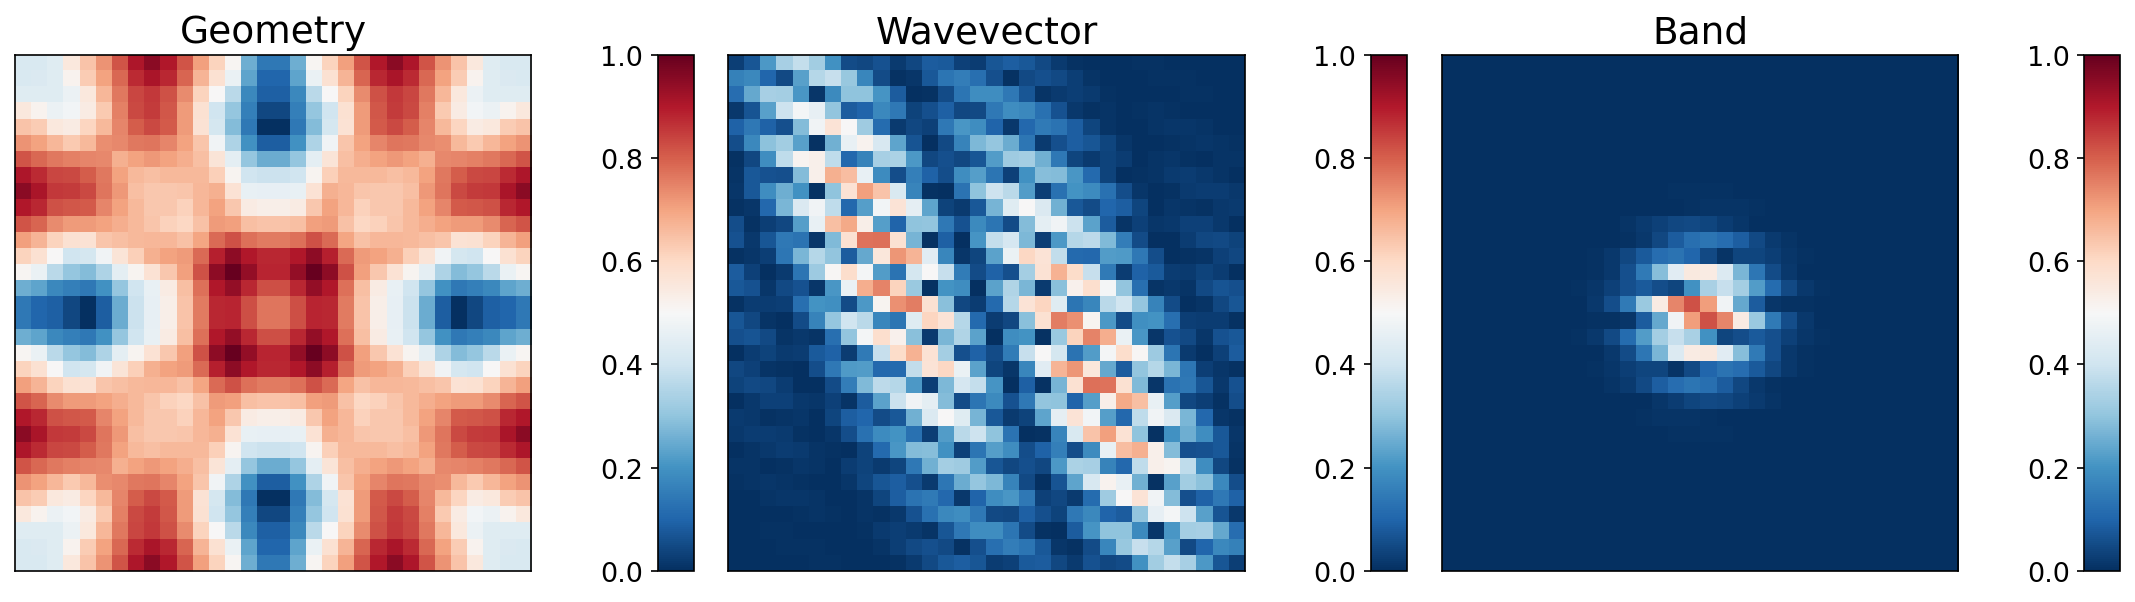
\includegraphics[width=\textwidth]{Figures/Fields C/c_test_nmae_p75_g279_w229_b3_input.png}
        \caption{Input sample at the 75th percentile of performance for unseen continuous valued geometries.}
        \label{fig:c_p75_input}
    \end{subfigure}
    \vspace{1em}
    \begin{subfigure}[c]{\textwidth}
    \centering
        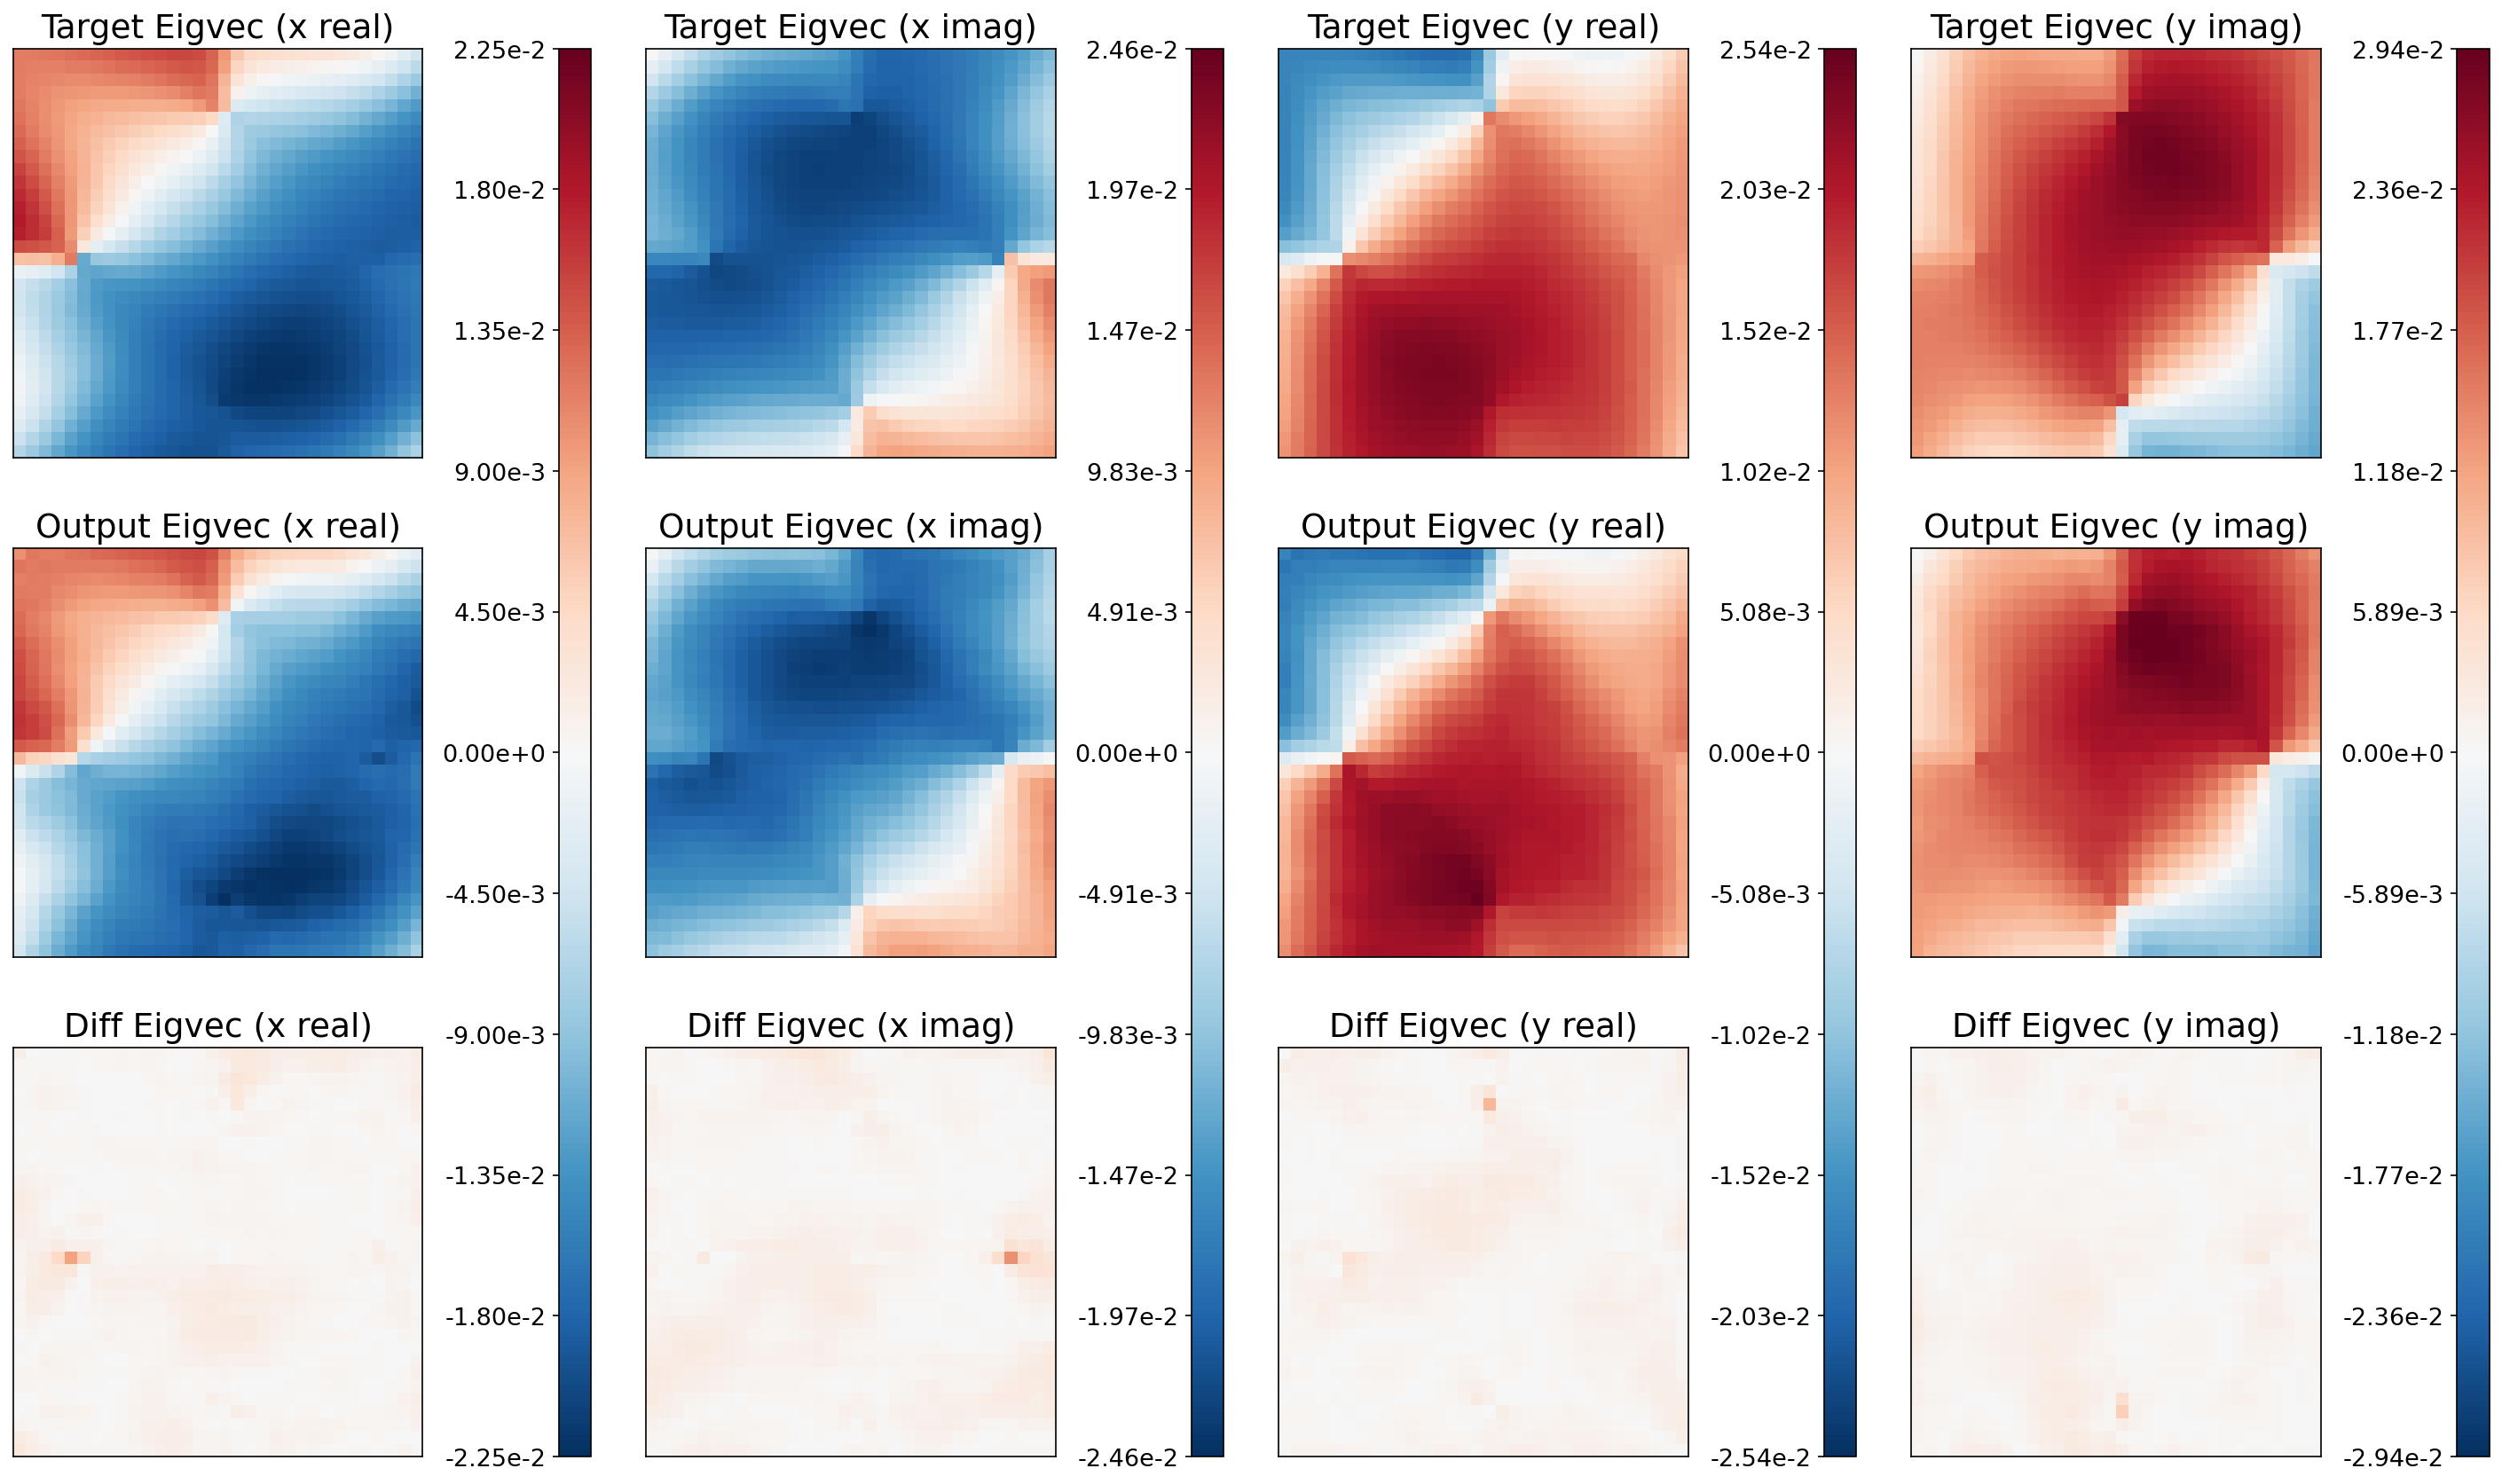
\includegraphics[width=\textwidth]{Figures/Fields C/c_test_nmae_p75_g279_w229_b3_fields.png}
        \caption{Output predictions at the 75th percentile of performance for unseen continuous valued geometries. The first row are target fields, followed by prediction fields on the second row, and difference fields on the third. At this point, the target and prediction are virtually indistinguishable by eye.}
        \label{fig:c_p75_output}
    \end{subfigure}
\end{figure}
These results demonstrate that with wavelet encodings, the FNO model performs well on continuous geometries, faithfully reproducing the displacement fields in most cases. Model predictions in the top three quartiles match targets well in structure and scale, with decreasing average pixel relative errors in the scale of $~10^{-2}$ smoothly decreasing down to $~10^{-4}$ with increasing percentile performance. (See Figure \ref{fig:loss_histogram_continuous} for more detailed statistics.)

\subsubsection{Discrete Geometries}
\begin{figure}[H]
    \centering
    \begin{subfigure}[c]{\textwidth}
        \centering
        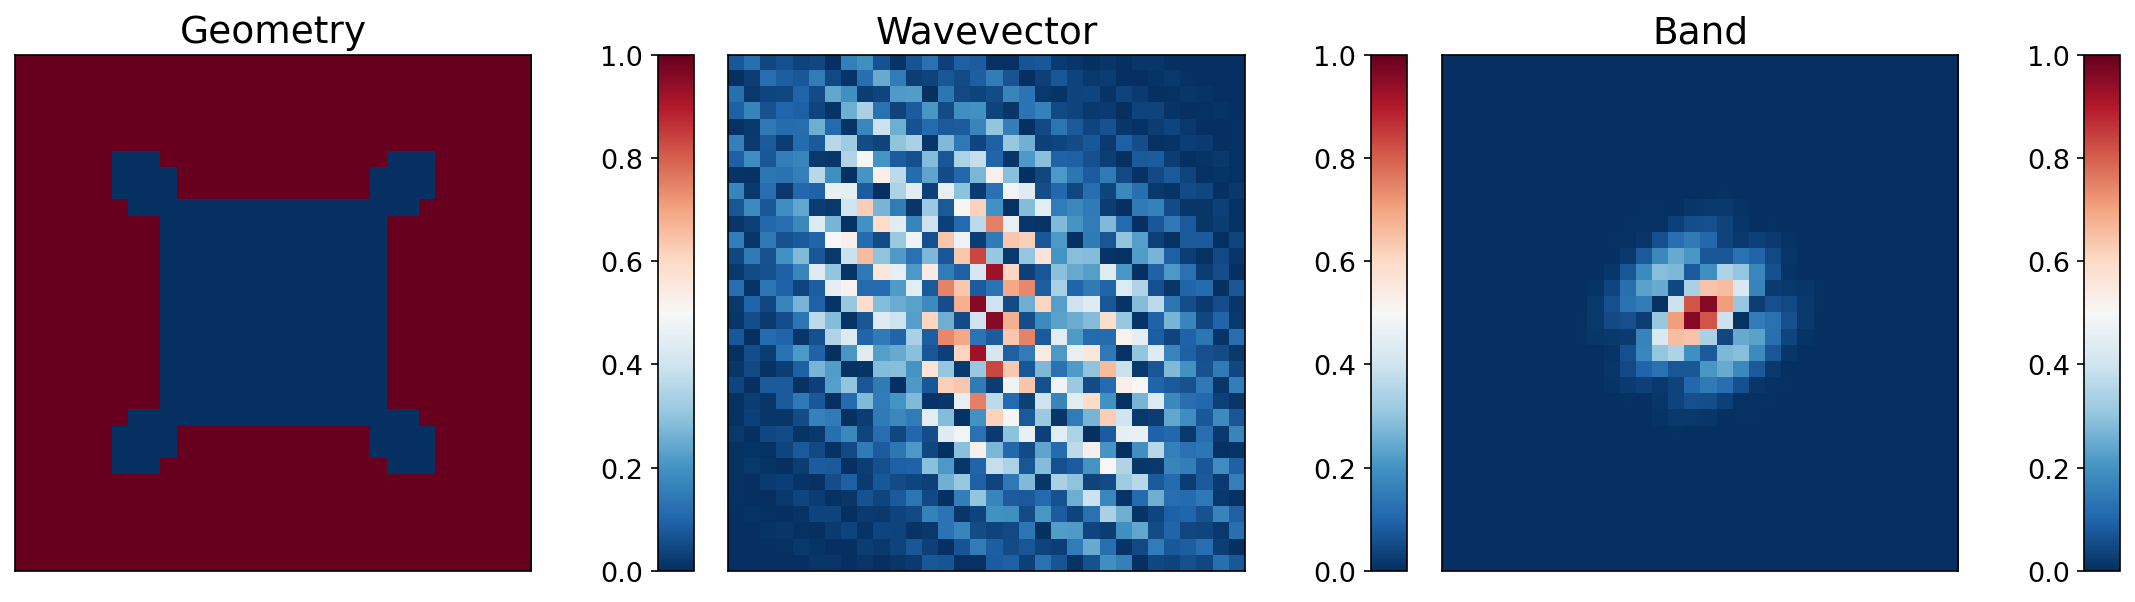
\includegraphics[width=0.75\textwidth]{Figures/Fields B/b_test_nmae_p25_g283_w234_b1_input.png}
        \caption{Input sample at the 25th percentile of performance for unseen discrete valued geometries.}
        \label{fig:b_p25_input}
    \end{subfigure}
    \vspace{1em}
    \begin{subfigure}[c]{\textwidth}
    \centering
        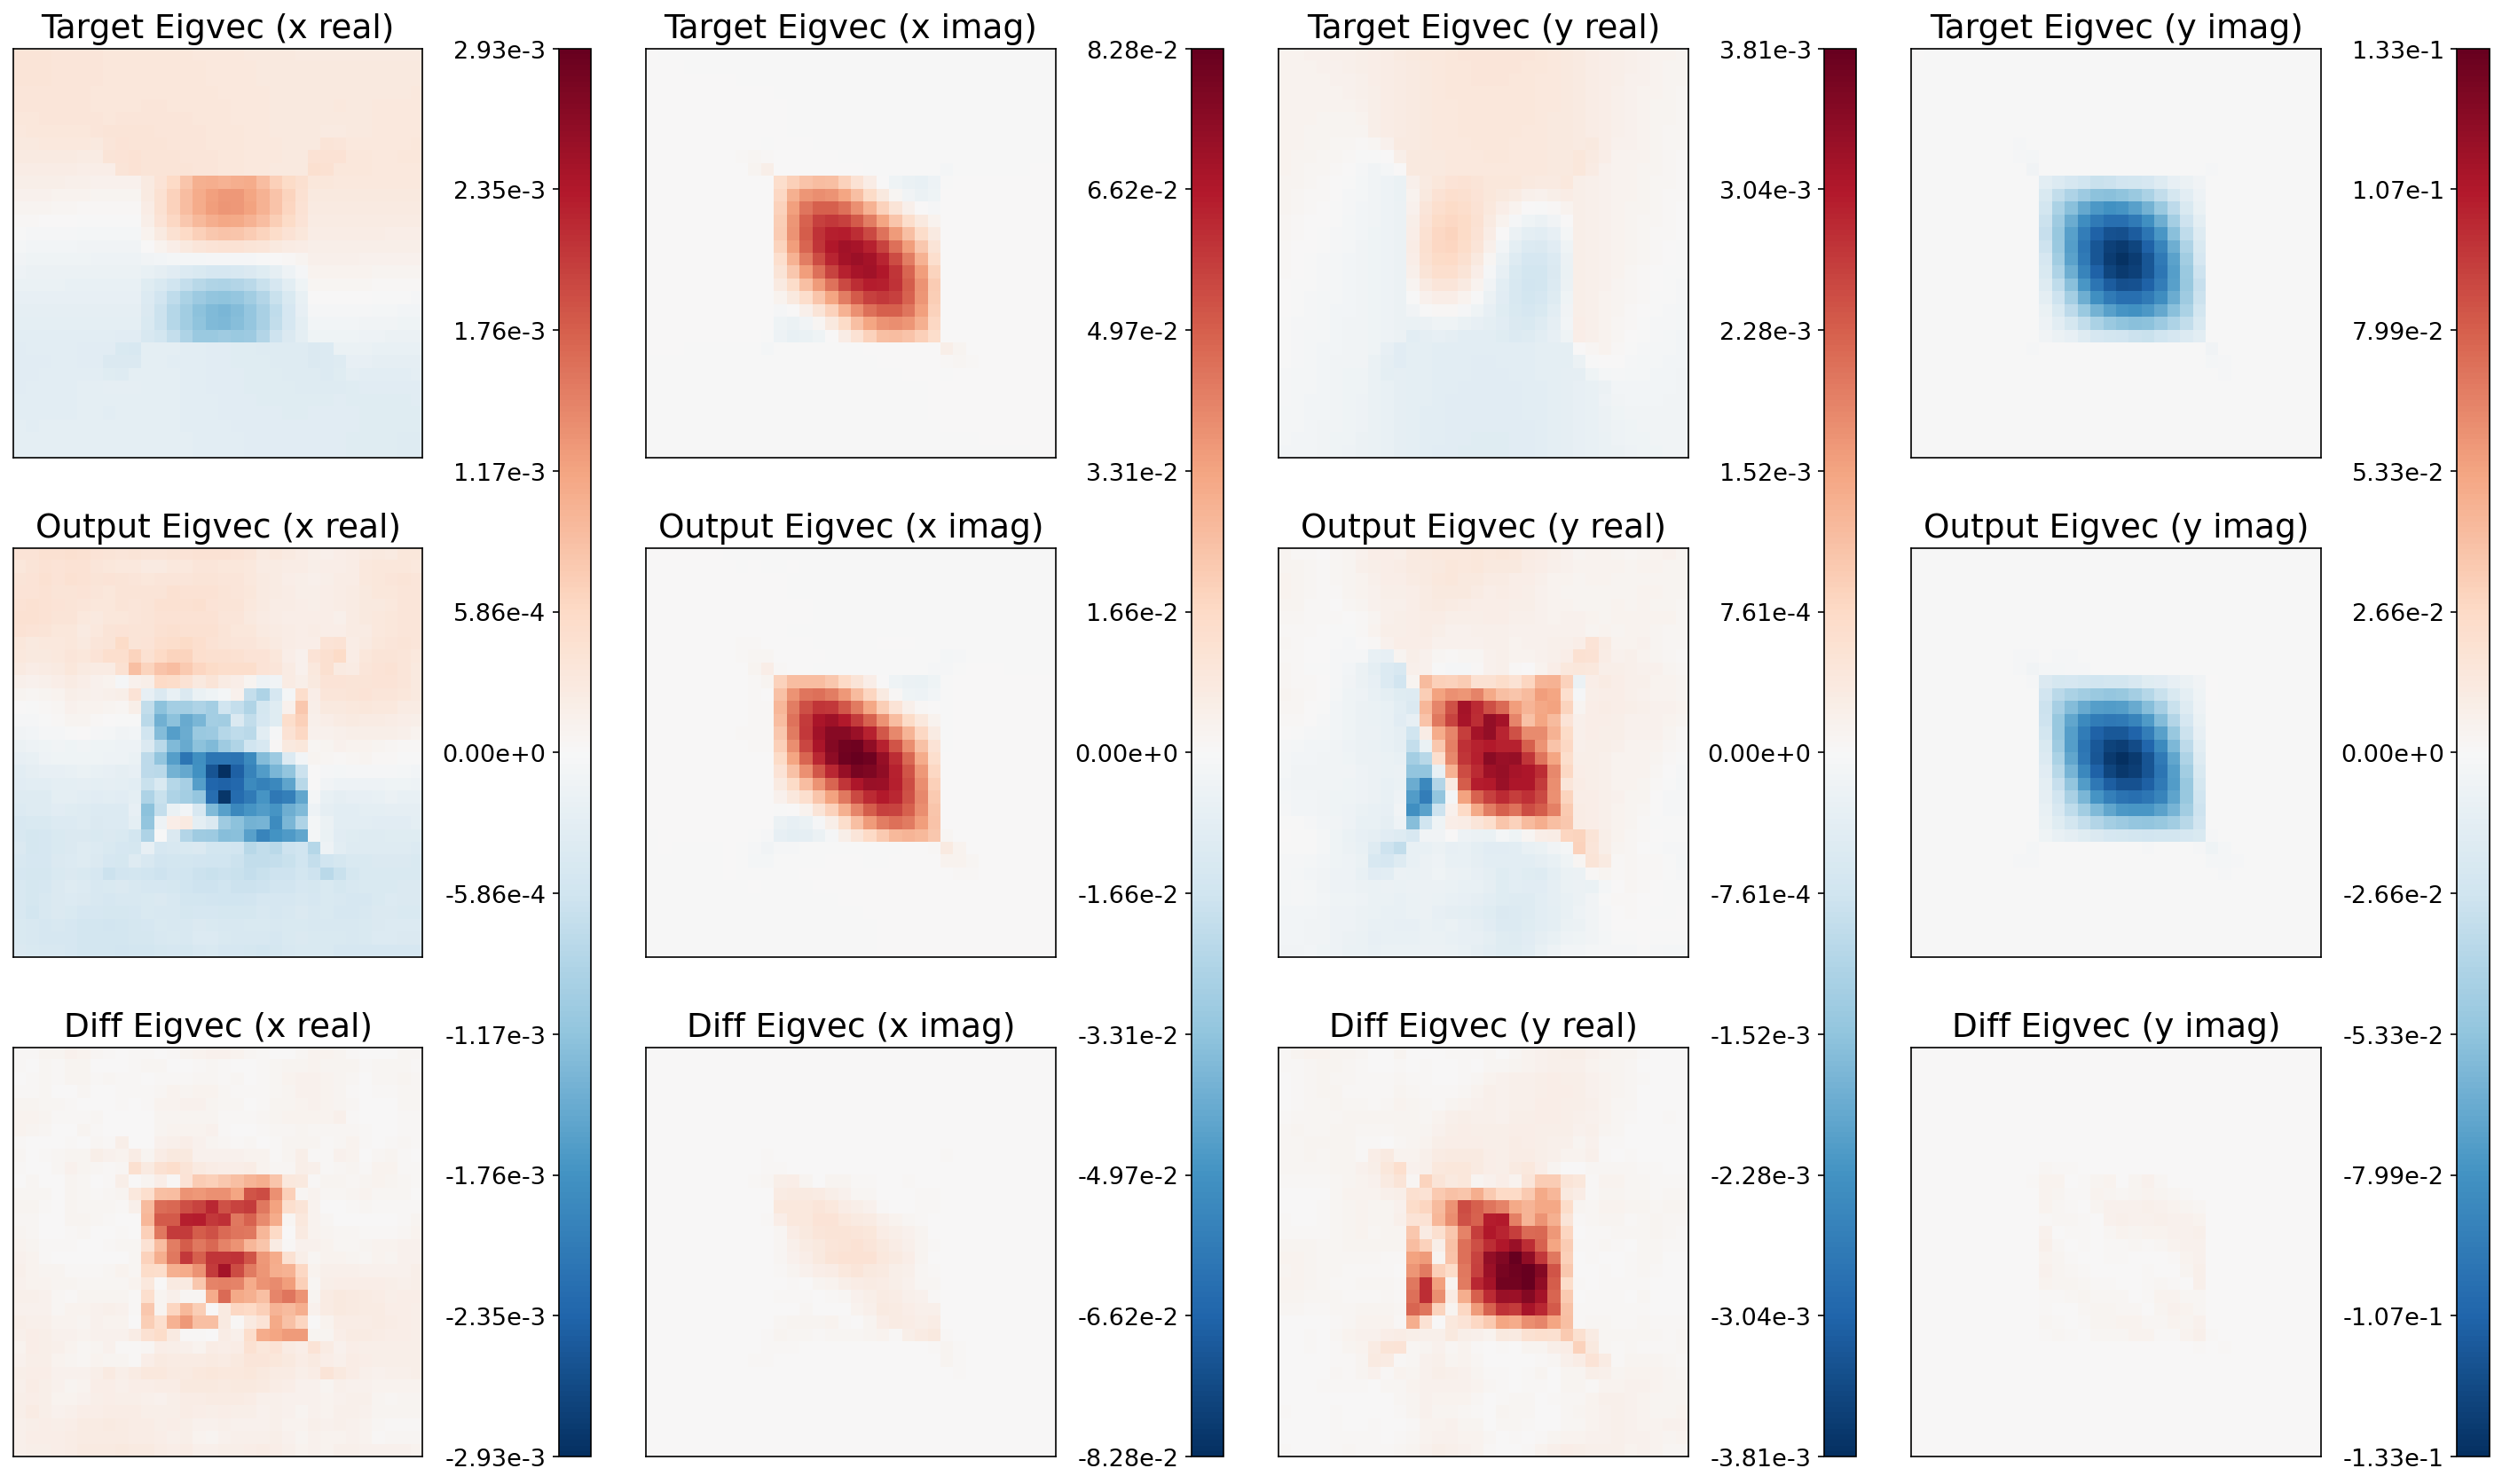
\includegraphics[width=\textwidth]{Figures/Fields B/b_test_nmae_p25_g283_w234_b1_fields.png}
        \caption{Output predictions at the 25th percentile of performance for unseen discrete valued geometries. The first row are target fields, followed by prediction fields on the second row, and difference fields on the third. Due to the nature of the loss function training, for this particular sample, the model would have prioritized the two imaginary displacement fields, because they are 1 to 2 orders of magnitude larger in scale compared to the two real displacement fields. In other words, absolute error is low at this point, but relative error is not for some channels of small scale than other channels. (Note that the colorbars for each column are independently scaled.)}
        \label{fig:b_p25_output}
    \end{subfigure}
\end{figure}

\begin{figure}[H]
    \centering
    \begin{subfigure}[c]{\textwidth}
        \centering
        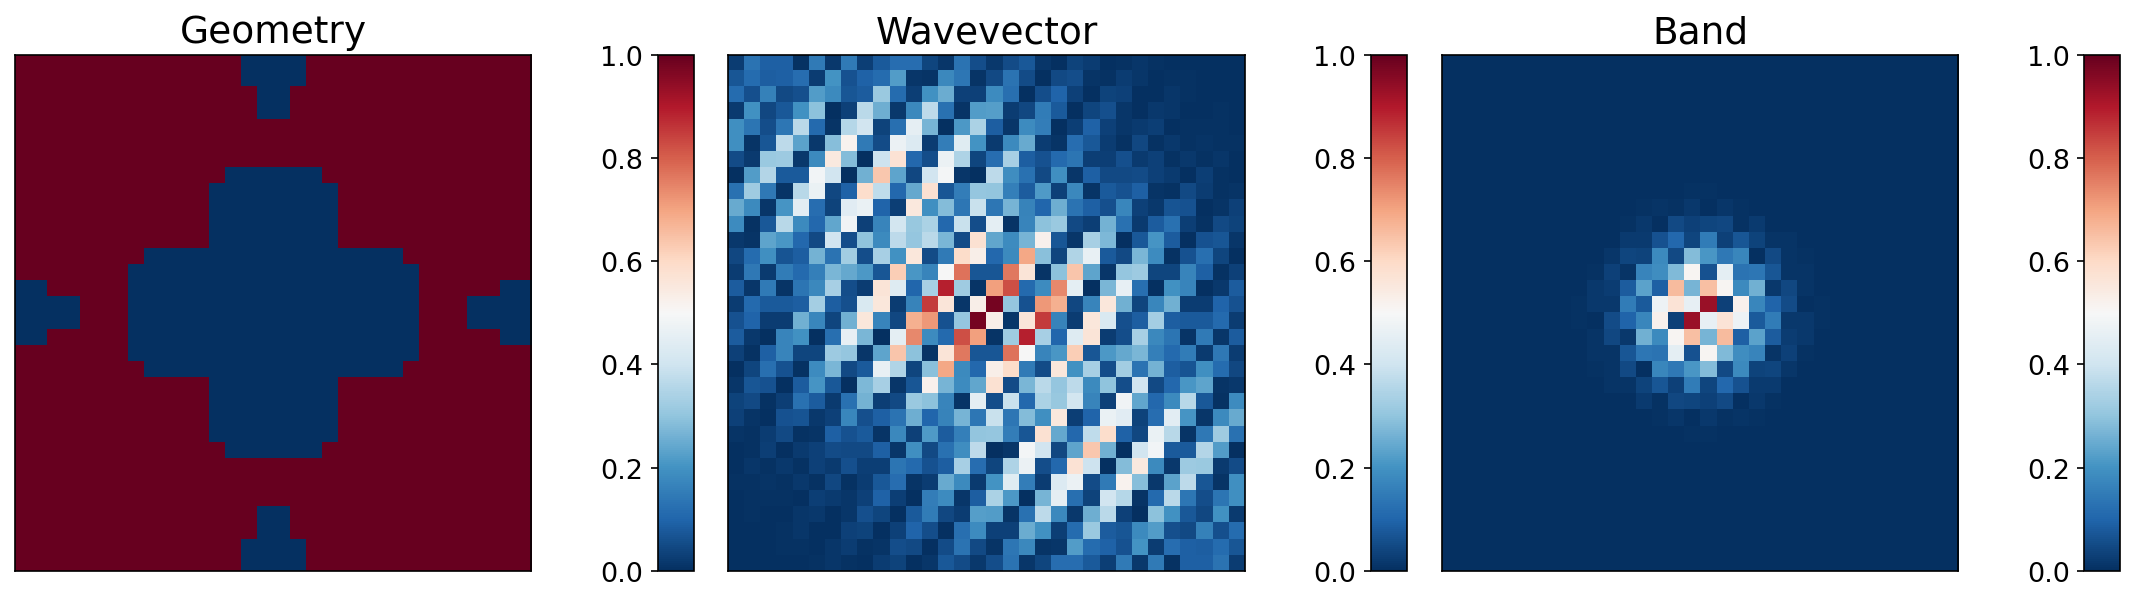
\includegraphics[width=0.75\textwidth]{Figures/Fields B/b_test_nmae_p50_g550_w257_b4_input.png}
        \caption{Input sample at the 50th percentile of performance for unseen discrete valued geometries.}
        \label{fig:b_p50_input}
    \end{subfigure}
    \vspace{1em}
    \begin{subfigure}[c]{\textwidth}
    \centering
        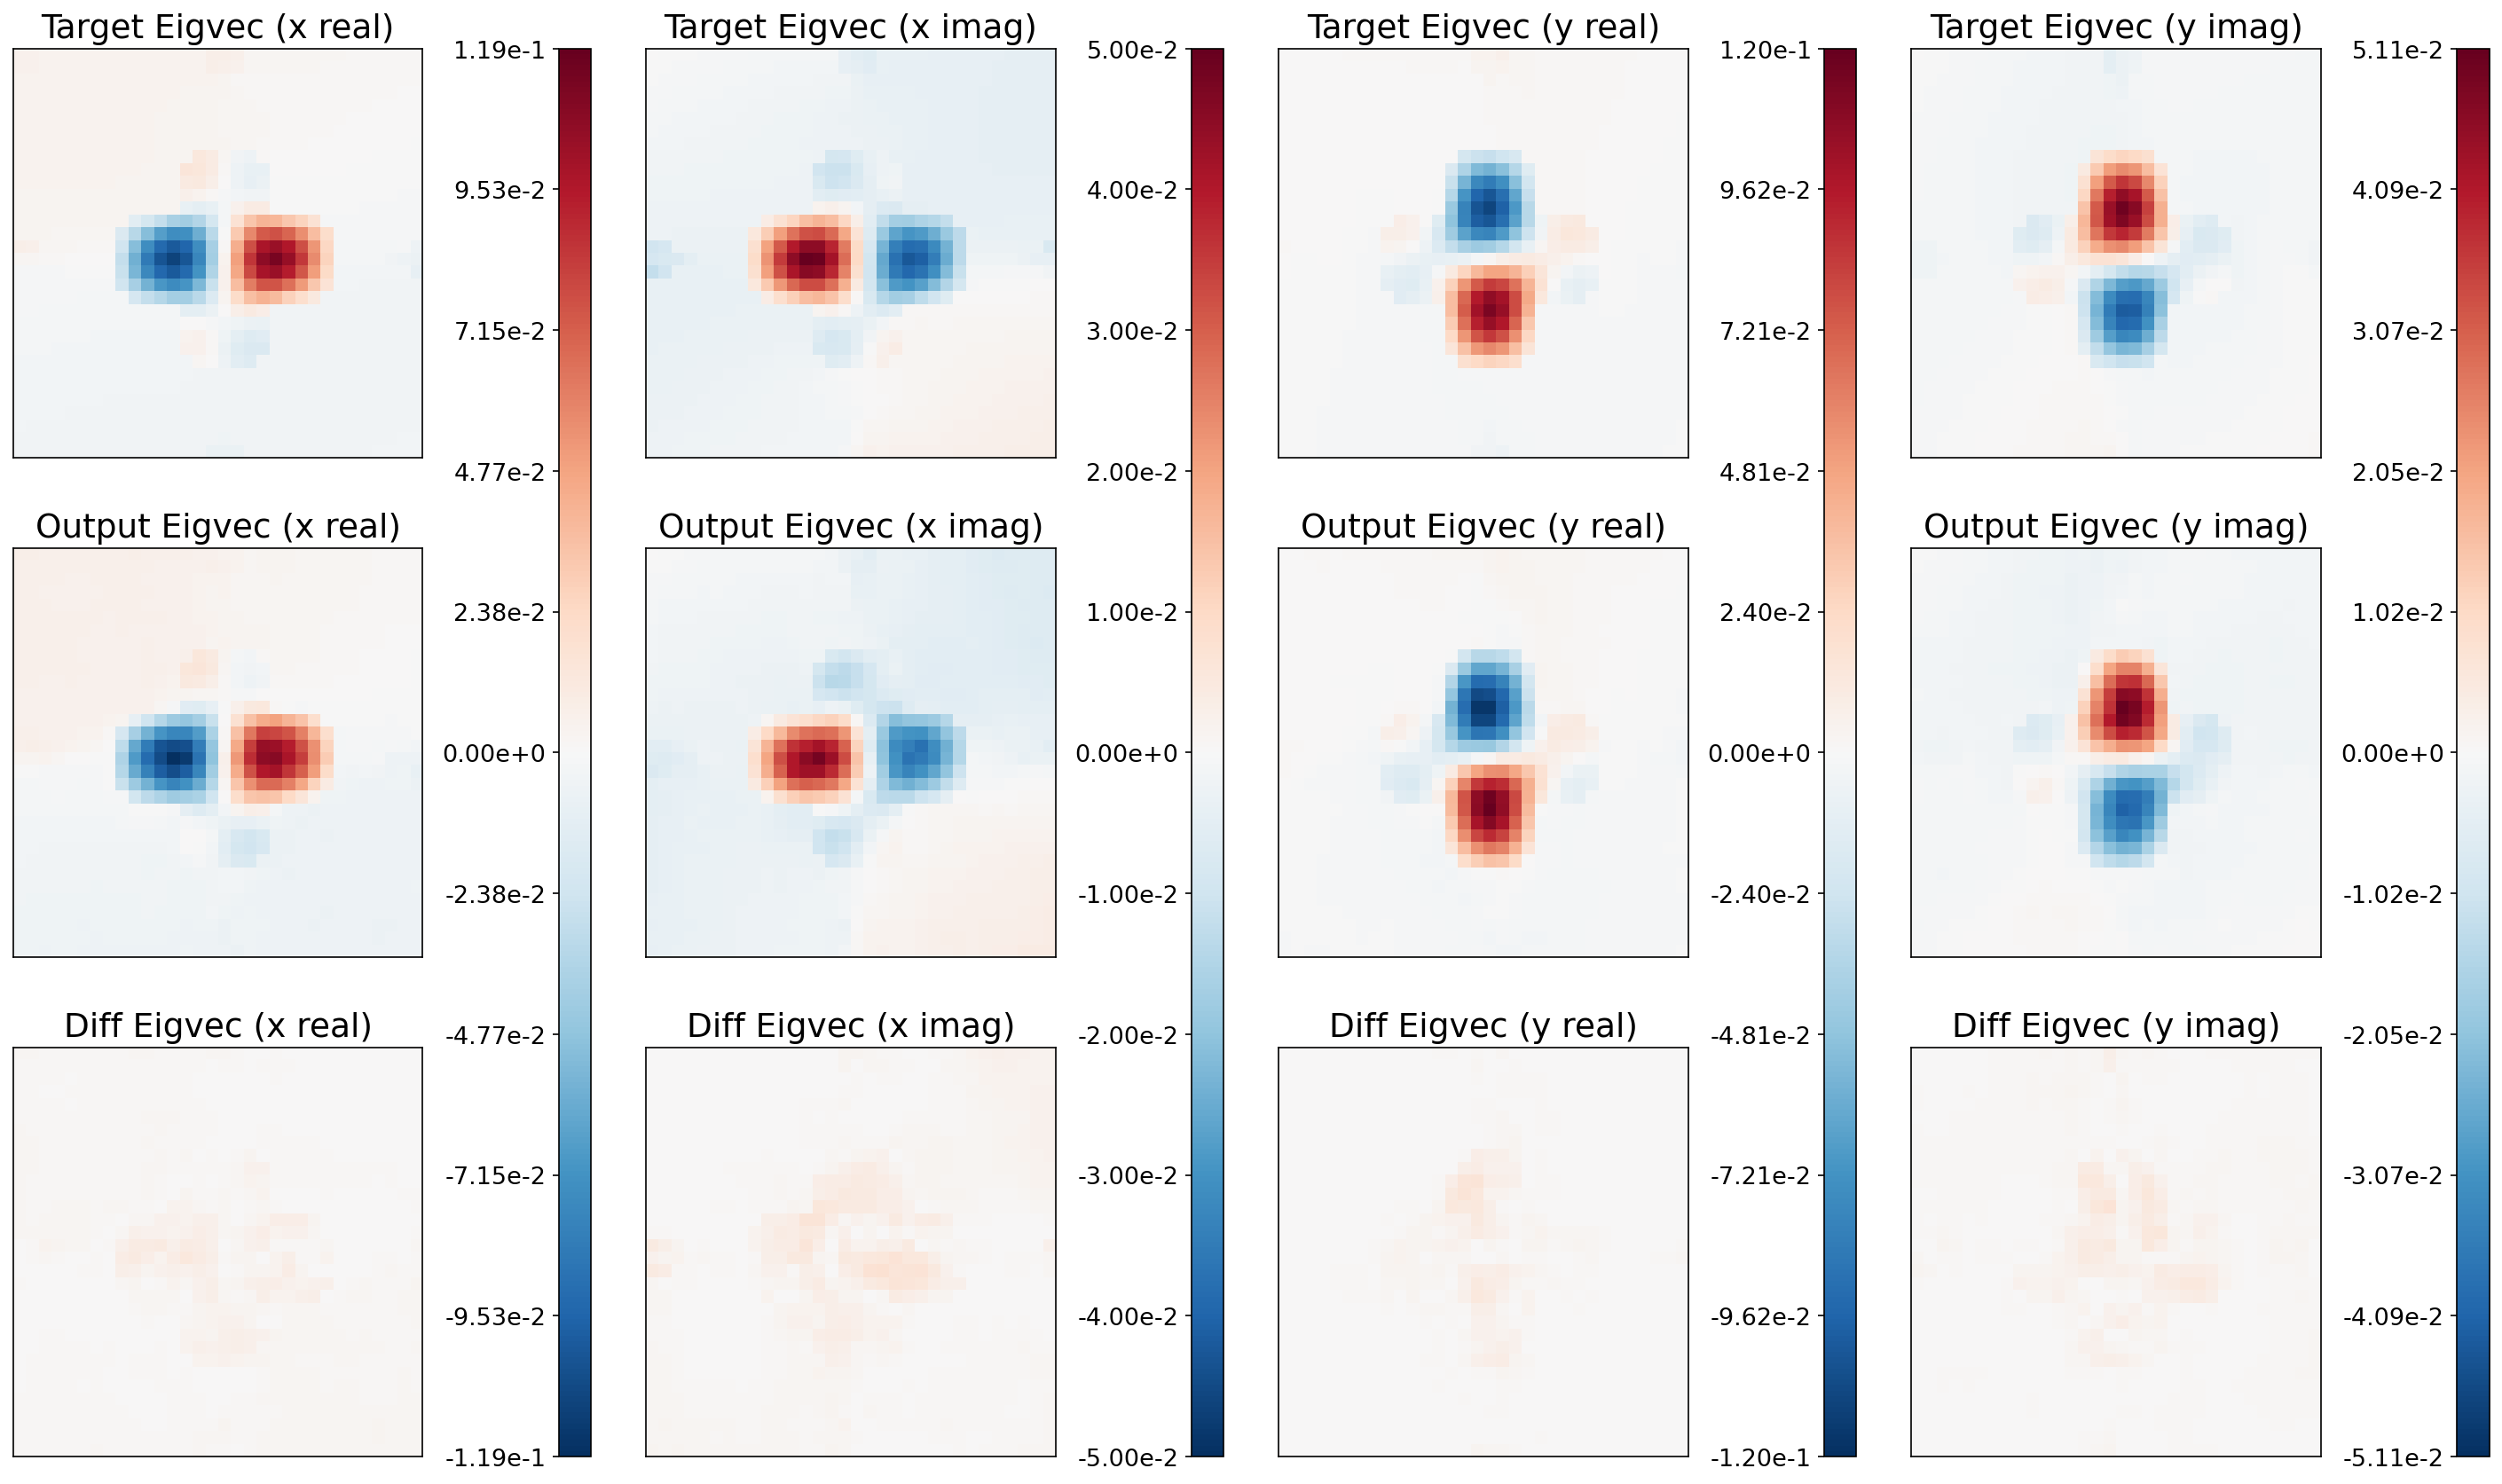
\includegraphics[width=\textwidth]{Figures/Fields B/b_test_nmae_p50_g550_w257_b4_fields.png}
        \caption{Output predictions at the 50th percentile of performance for unseen discrete valued geometries. The first row are target fields, followed by prediction fields on the second row, and difference fields on the third. At this point, absolute and relative errors are low and there is high agreement in structural and scale between targets and predictions.}
        \label{fig:b_p50_output}
    \end{subfigure}
\end{figure}

\begin{figure}[H]
    \centering
    \begin{subfigure}[c]{\textwidth}
        \centering
        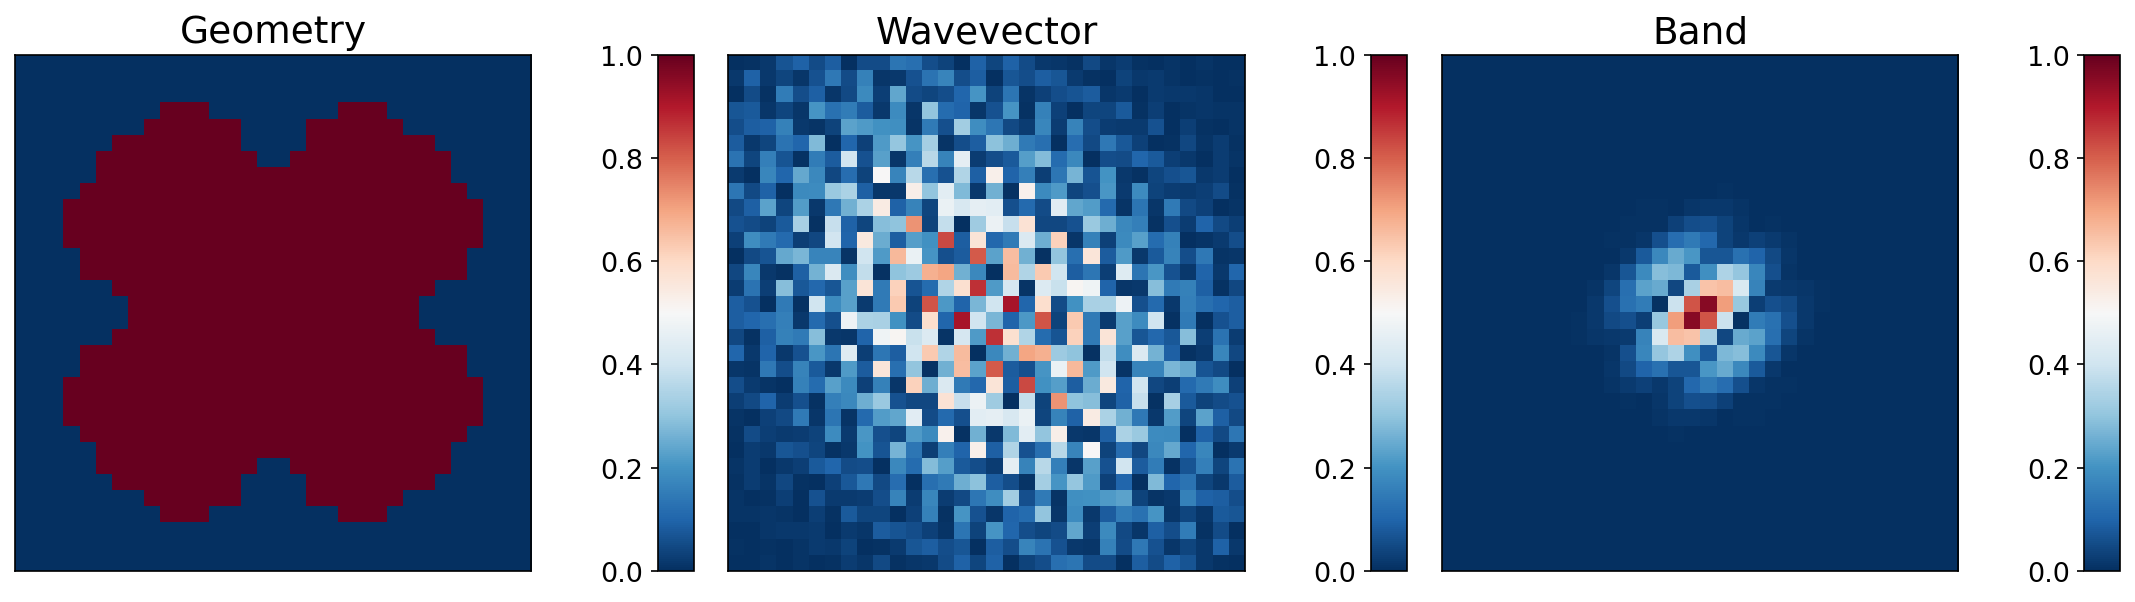
\includegraphics[width=0.75\textwidth]{Figures/Fields B/b_test_nmae_p75_g234_w145_b1_input.png}
        \caption{Input sample at the 75th percentile of performance for unseen discrete valued geometries.}
        \label{fig:b_p75_input}
    \end{subfigure}
    \vspace{1em}
    \begin{subfigure}[c]{\textwidth}
    \centering
        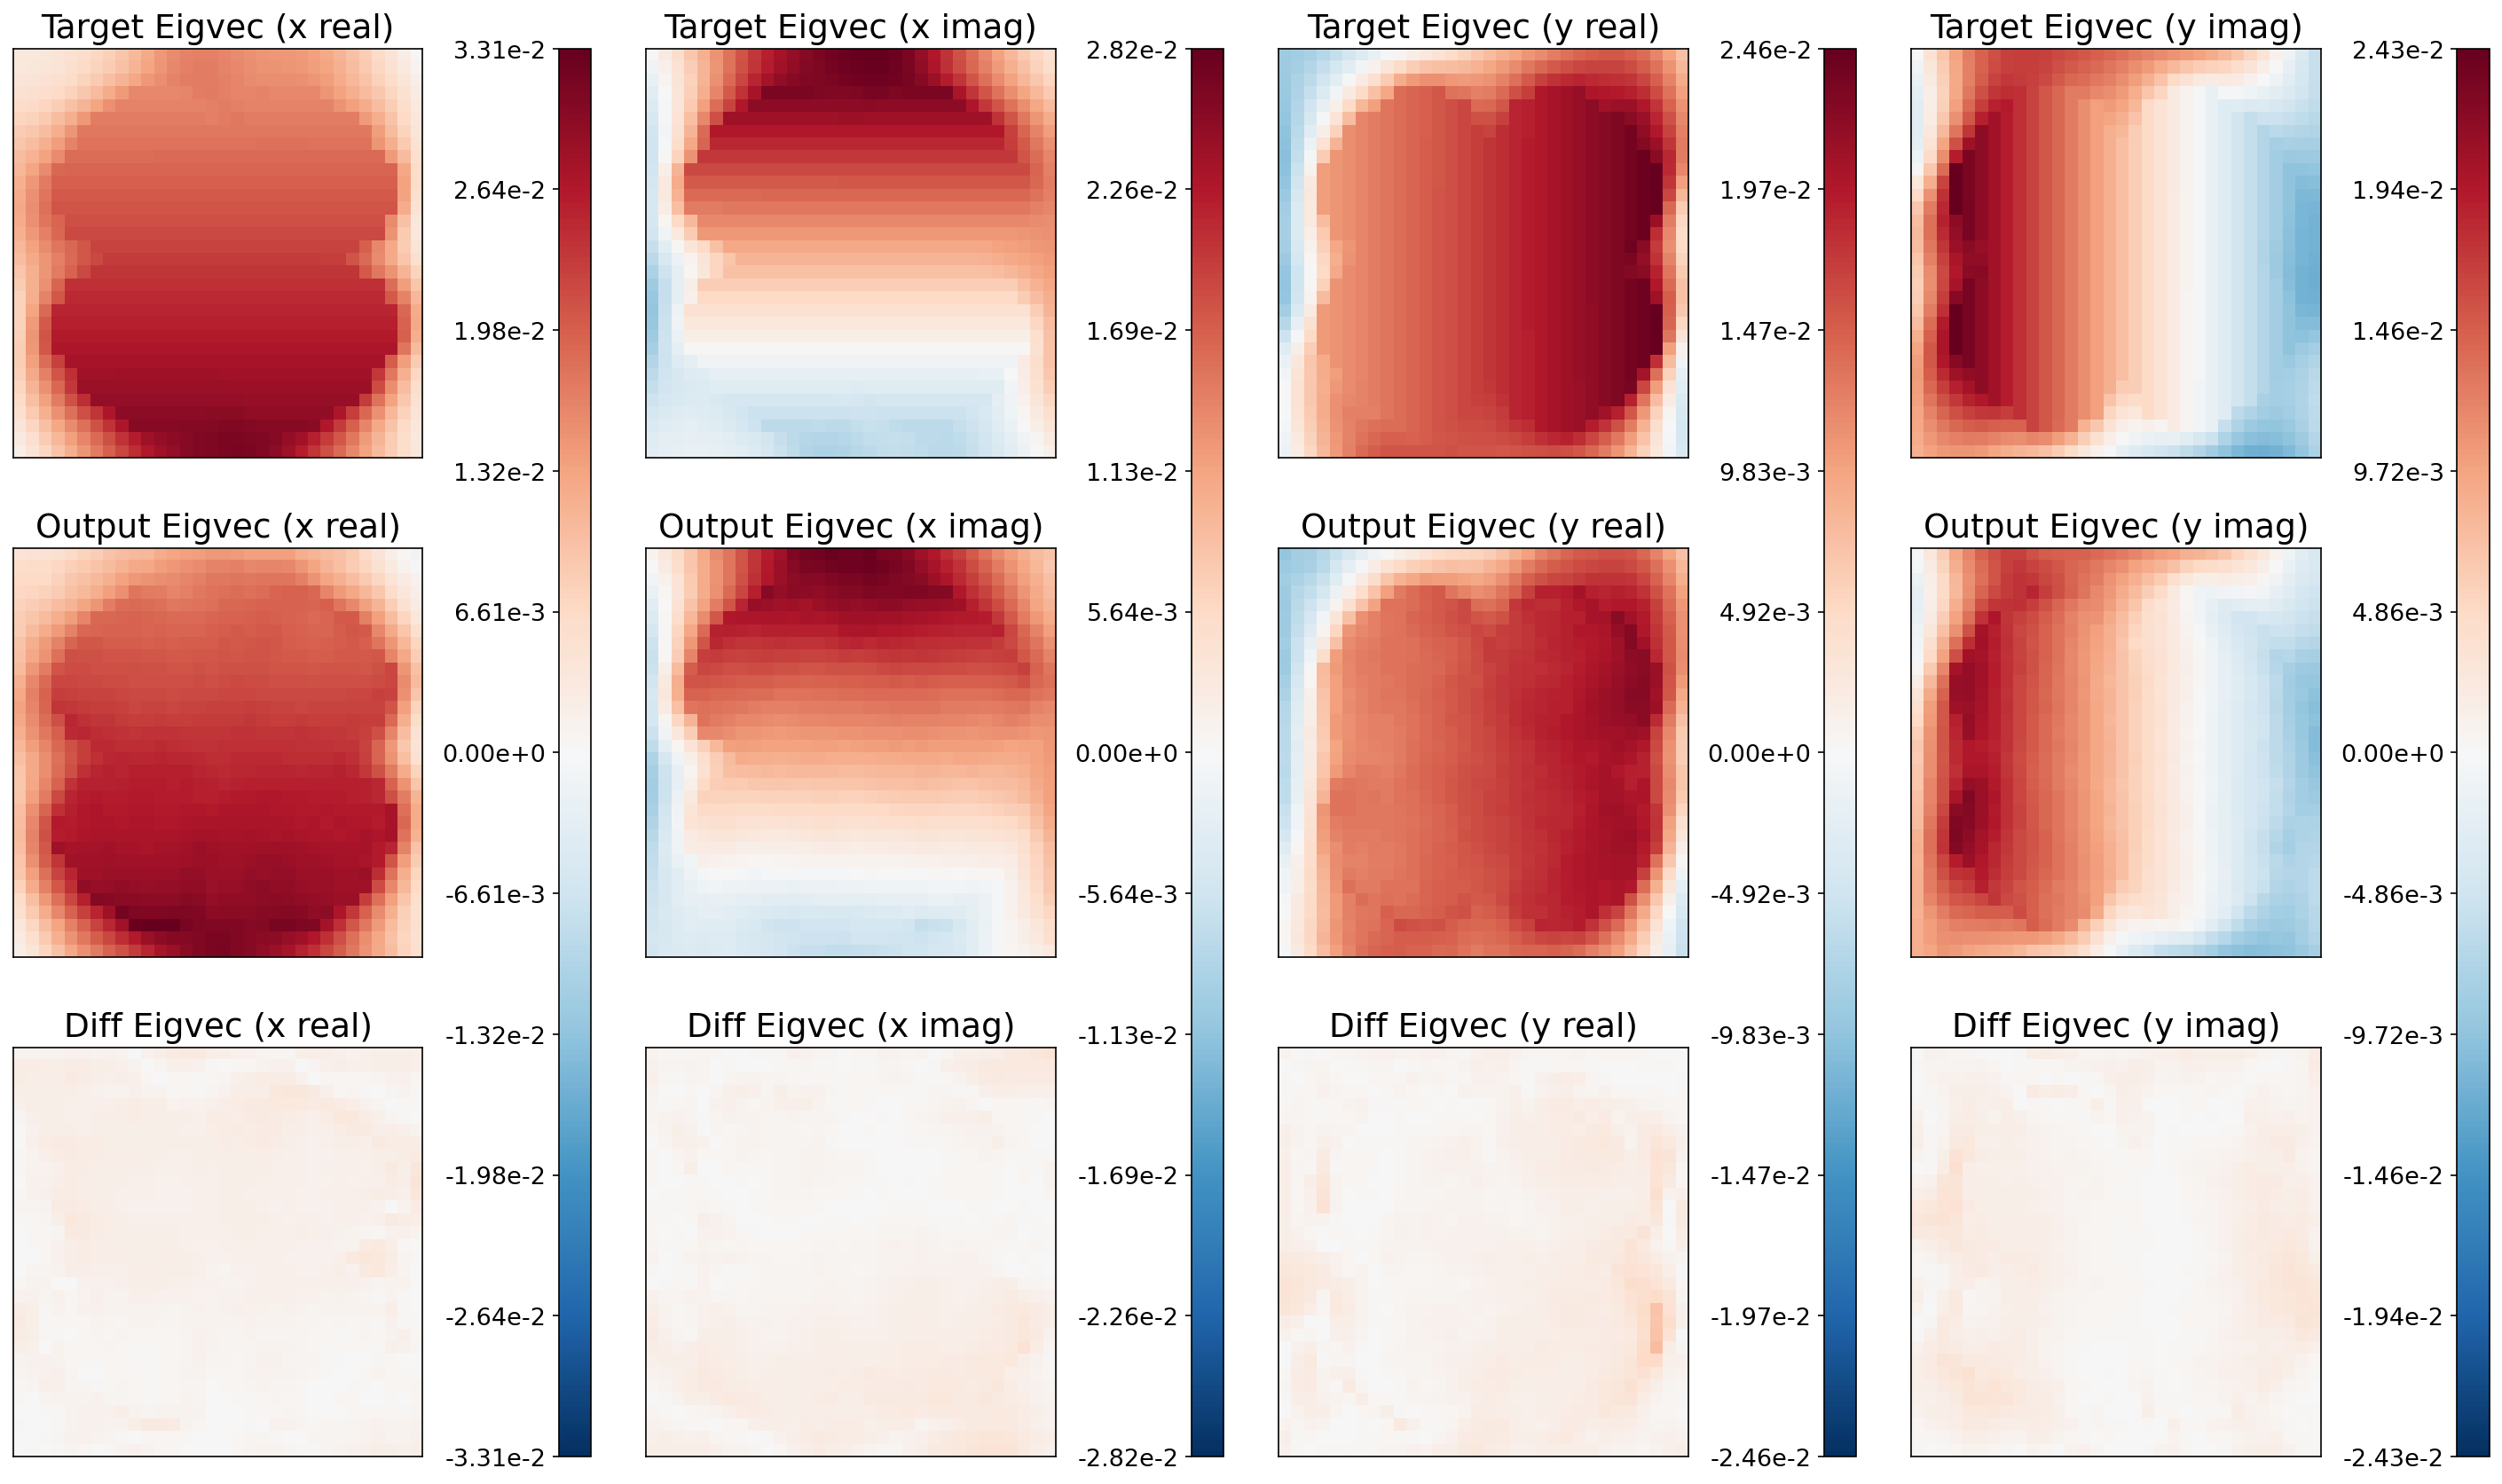
\includegraphics[width=\textwidth]{Figures/Fields B/b_test_nmae_p75_g234_w145_b1_fields.png}
        \caption{Output predictions at the 75th percentile of performance for unseen discrete valued geometries. The first row are target fields, followed by prediction fields on the second row, and difference fields on the third. At this point, disagreements between targets and predictions become very hard to see by eye.}
        \label{fig:b_p75_output}
    \end{subfigure}
\end{figure}

Like with the continuous geometry case, these results demonstrate that with wavelet encodings, the FNO model performs well on discrete geometries, faithfully reproducing the displacement fields in most cases. Model predictions in the top three quartiles match targets well in structure and scale, with decreasing average pixel relative errors in the scale of $~10^{-2}$ smoothly decreasing down to $~10^{-4}$ with increasing percentile performance. (See Figure \ref{fig:loss_histogram_discrete} for more detailed statistics.)

\subsubsection{Continuous Versus Discrete Performance}
The model being able to simultaneously predict well on both continuous and discrete geometries is a non-trivial and important takeaway for the capabilities of FNOs with paired with wavelet encodings. Prior encoding strategies of constant fields and sinusoidal fields delivered far worse results with grainy structures or mode collapse issues because conditioning constants (wavevector and band) information could not propagate well through the spectral branch of the FNO layers. The performance over all unseen samples in the test set are shown in \ref{fig:loss_histograms}. 

The poorer performance on binarized geometries is consistent with basic operator-learning theory. Continuous material fields lie in smoother function classes, whereas binary two-phase designs contain jump discontinuities with nonexistent derivatives at material interfaces. Since an FNO approximates the FEA operator $\mathcal{G}: \mathcal{U}\to\mathcal{V}$ through truncated Fourier representations, it is naturally advantaged when both inputs and outputs are comparatively smooth. Discrete geometries thus perform worse due to sharp boundaries, localized gradients, and broadband high-wavenumber content that are poorly captured on a fixed $32\times32$ grid and are mismatched to smooth wavelet encodings. Additionally, because continuous geometries have a greater tendency to have large sections of fields with zero or low displacements, a small spike is seen in relative error performance due to the near zero displacements which results in a small denominator.

These results indicate two important takeaways. The first is that it is possible for FNOs with wavelet encodings to learn multiple deformation modes for each geometry which the user can toggle between arbitrarily by setting the wavevector and band inputs. This is to our knowledge the first demonstration of FNOs on solving eigenvalue PDEs. The second, is that it is possible for that same model to simultaneously learn very different distributions of geometries (continuous valued and discrete valued), indicating it might be possible to distill out a generalized understanding of the PDE itself independent of geometry distributions and statistical artifacts. This is a possible subject for future work.

\begin{figure}[H]
    \centering
    \begin{subfigure}[t]{0.49\textwidth}
        \centering
        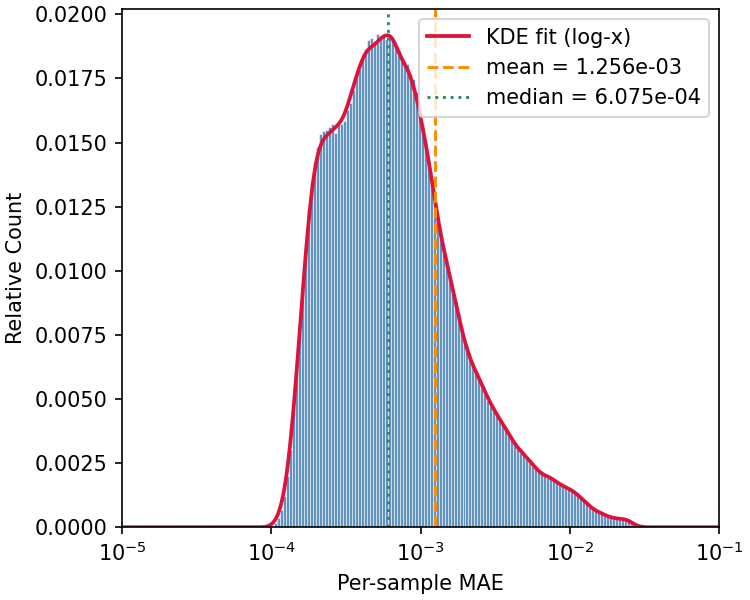
\includegraphics[width=\textwidth]{Figures/Statistics/displacement_loss_histogram_mae_c_test.png}
        \caption{Performance histogram for continuous geometries.}
        \label{fig:disp_loss_histogram_continuous}
    \end{subfigure}
    \hfill
    \begin{subfigure}[t]{0.49\textwidth}
        \centering
        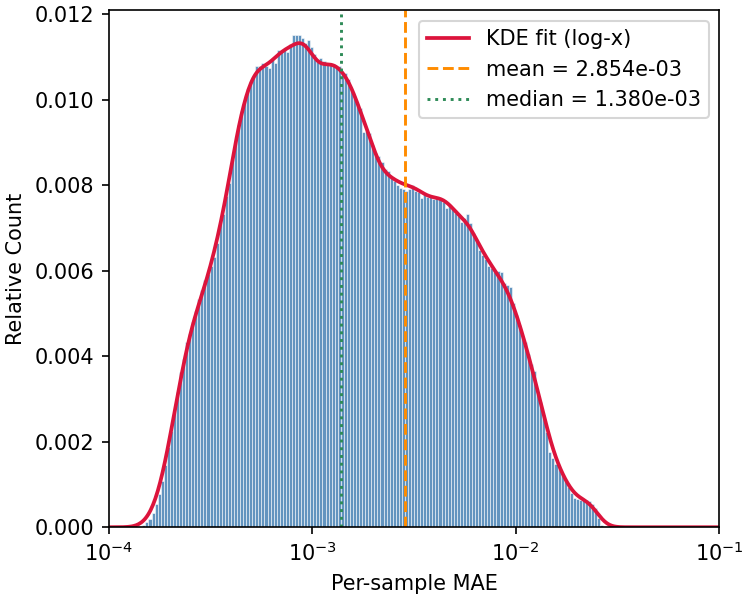
\includegraphics[width=\textwidth]{Figures/Statistics/displacement_loss_histogram_mae_b_test.png}
        \caption{Performance histogram for discrete geometries.}
        \label{fig:disp_loss_histogram_discrete}
    \end{subfigure}
    \caption{Comparison of relative prediction error distributions for continuous-valued and discrete metamaterial geometries for the same model. While there are some tail outliers, most samples fall within the range of $~10^{-2}$ to $~10^{-4}$, indicating that the same model is able to learn continuous and discrete geometry cases.}
    \label{fig:disp_loss_histograms}
\end{figure}

%%%%%%%%%%%%%%%%%%%%%%%%%%%%%%%%%%%%%%%%%%%%%%%%%%%%%%%%%%%%%%%%%%%%%%
\subsection{Dispersion Band Reconstruction}
\begin{figure}[H]
    \centering
    \begin{subfigure}[t]{0.32\textwidth}
        \centering
        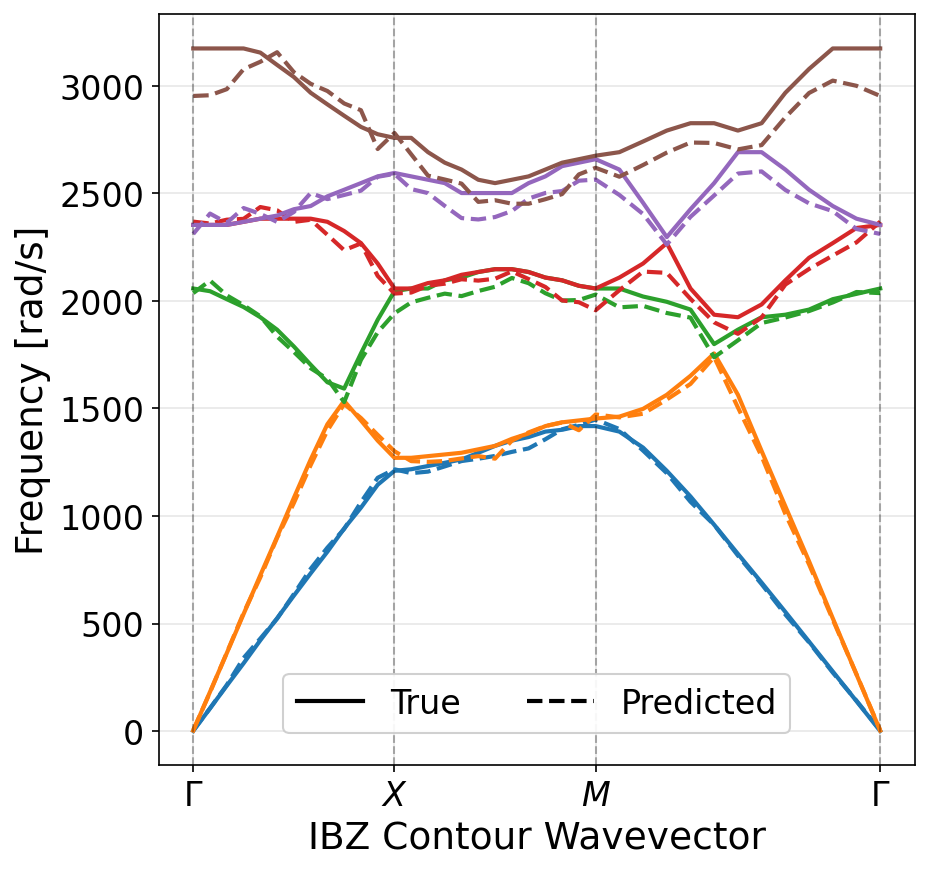
\includegraphics[width=\textwidth]{Figures/Dispersion C/NMAE753_NMSE730_g597.png}
        \caption{25th percentile performance.}
        \label{fig:dispersion_c_p25}
    \end{subfigure}
    \hfill
    \begin{subfigure}[t]{0.32\textwidth}
        \centering
        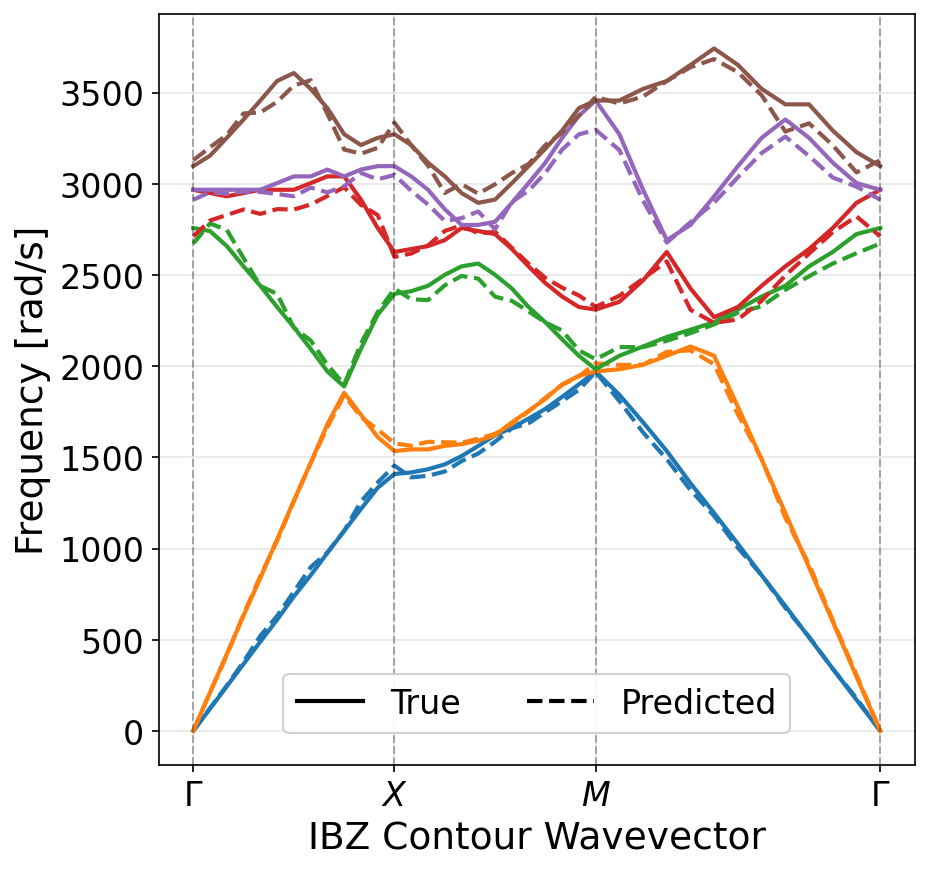
\includegraphics[width=\textwidth]{Figures/Dispersion C/NMAE502_NMSE443_g182.png}
        \caption{50th percentile performance.}
        \label{fig:dispersion_c_p50}
    \end{subfigure}
    \hfill
    \begin{subfigure}[t]{0.32\textwidth}
        \centering
        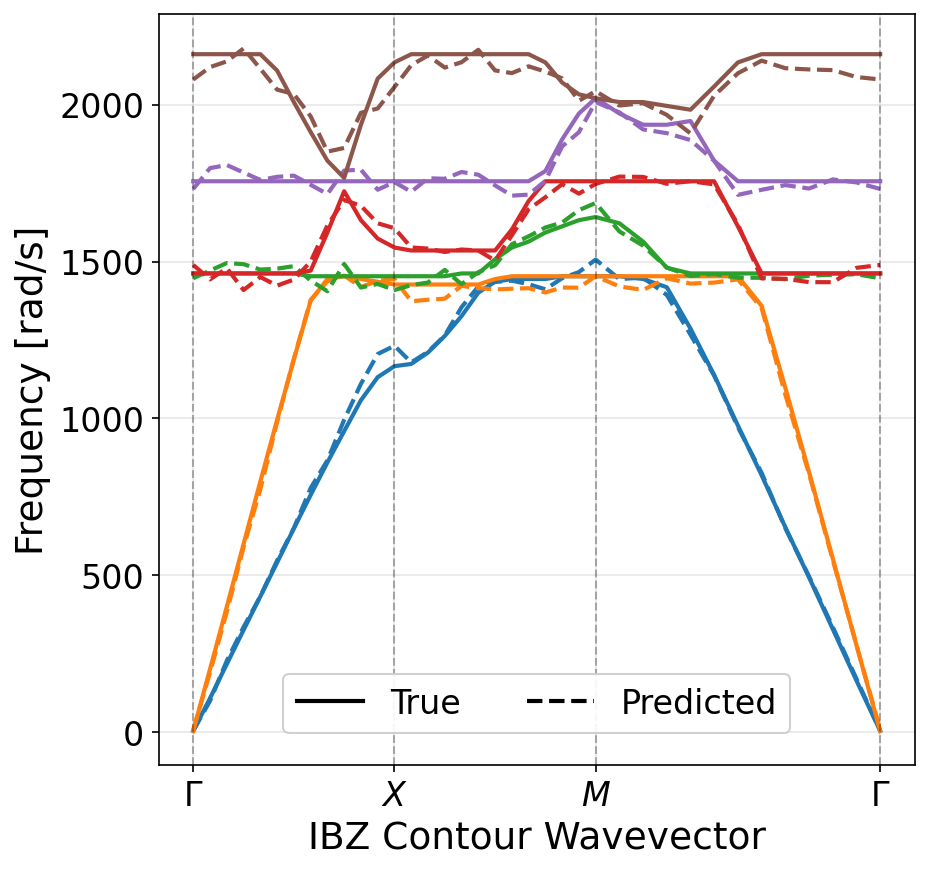
\includegraphics[width=\textwidth]{Figures/Dispersion C/NMAE250_NMSE250_g928.png}
        \caption{75th percentile performance.}
        \label{fig:dispersion_c_p75}
    \end{subfigure}
    \caption{Predicted and ground-truth dispersion bands for representative unseen continuous valued geometries spanning the 25th, 50th, and 75th percentiles of prediction performance.}
    \label{fig:dispersion_c_percentiles}
\end{figure}
These plots represent the eigenfrequency predictions of the model across all 325 wavevectors forming the half plane for continuous valued geometries, downselected to be the horizontal, vertical, and diagonal traversal of the IBZ. Note that because the encoding of the eigenfrequency into a field has a log operation (to allow the model to learn relationships at multiple scales), errors tend to be relative to the scale of the target, and thus higher bands may seem to be more deviant on a linear scale plot. Overall, the model performance is quite good at predictions in the encoded eigenfrequency, showing an average of < 1\% prediction error across all unseen samples.

\begin{figure}[H]
    \centering
    \begin{subfigure}[t]{0.32\textwidth}
        \centering
        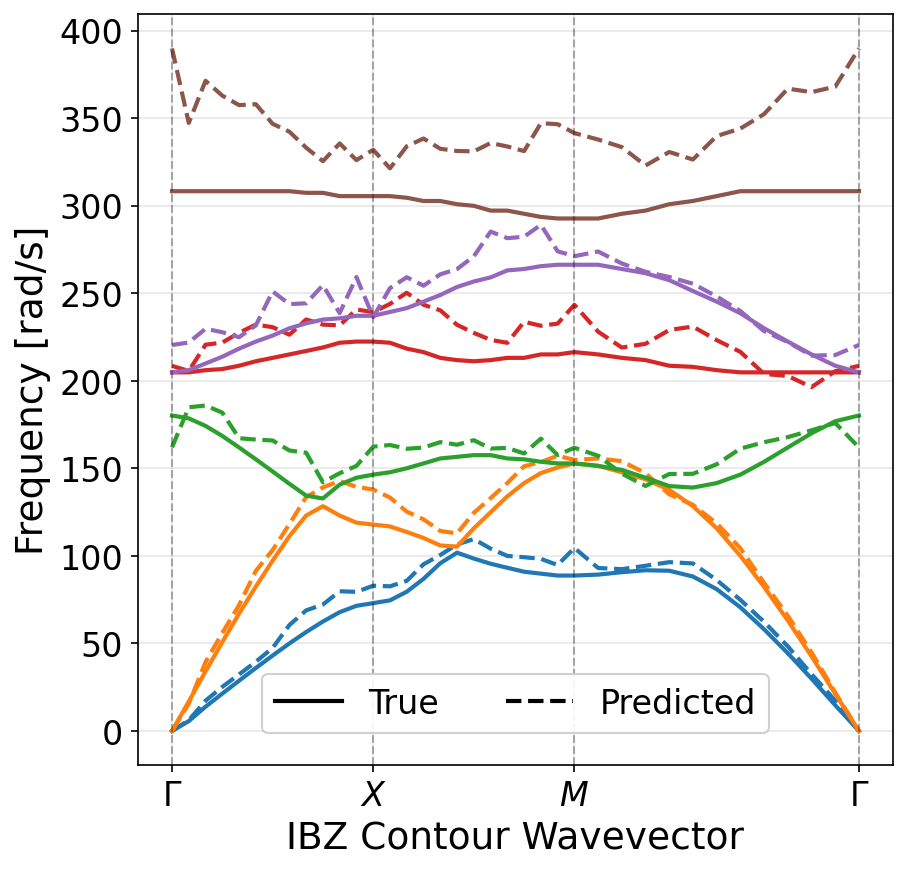
\includegraphics[width=\textwidth]{Figures/Dispersion B/NMAE754_NMSE754_g690.png}
        \caption{25th percentile performance.}
        \label{fig:dispersion_b_p25}
    \end{subfigure}
    \hfill
    \begin{subfigure}[t]{0.32\textwidth}
        \centering
        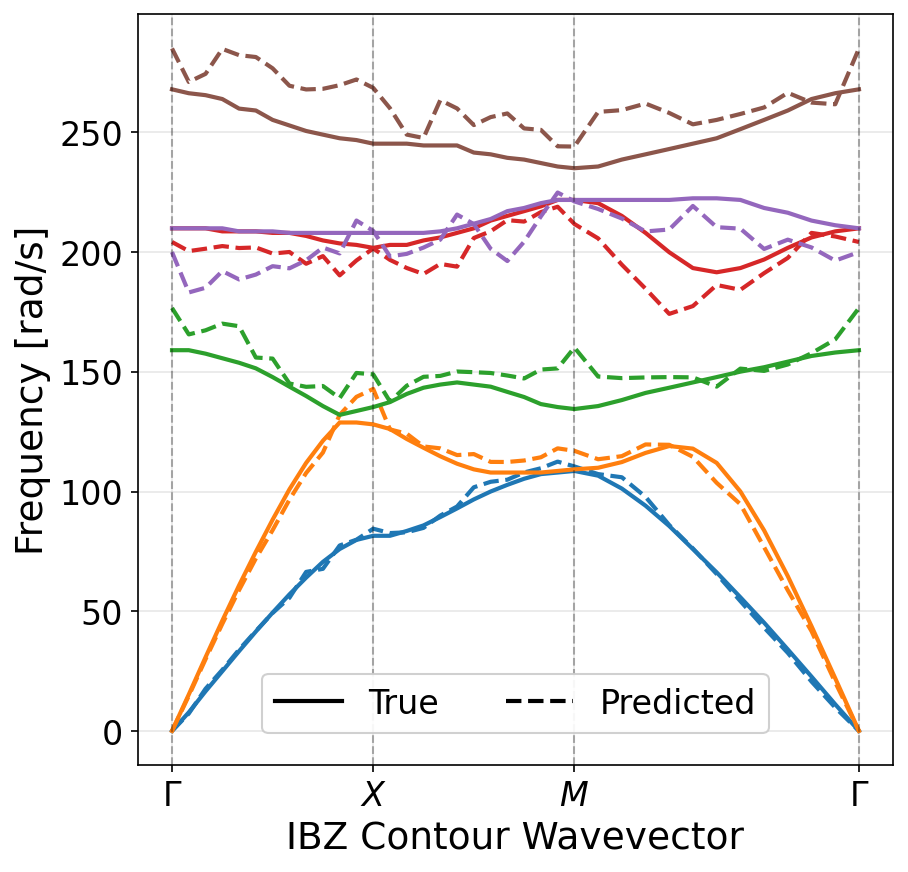
\includegraphics[width=\textwidth]{Figures/Dispersion B/NMAE499_NMSE514_g975.png}
        \caption{50th percentile performance.}
        \label{fig:dispersion_b_p50}
    \end{subfigure}
    \hfill
    \begin{subfigure}[t]{0.32\textwidth}
        \centering
        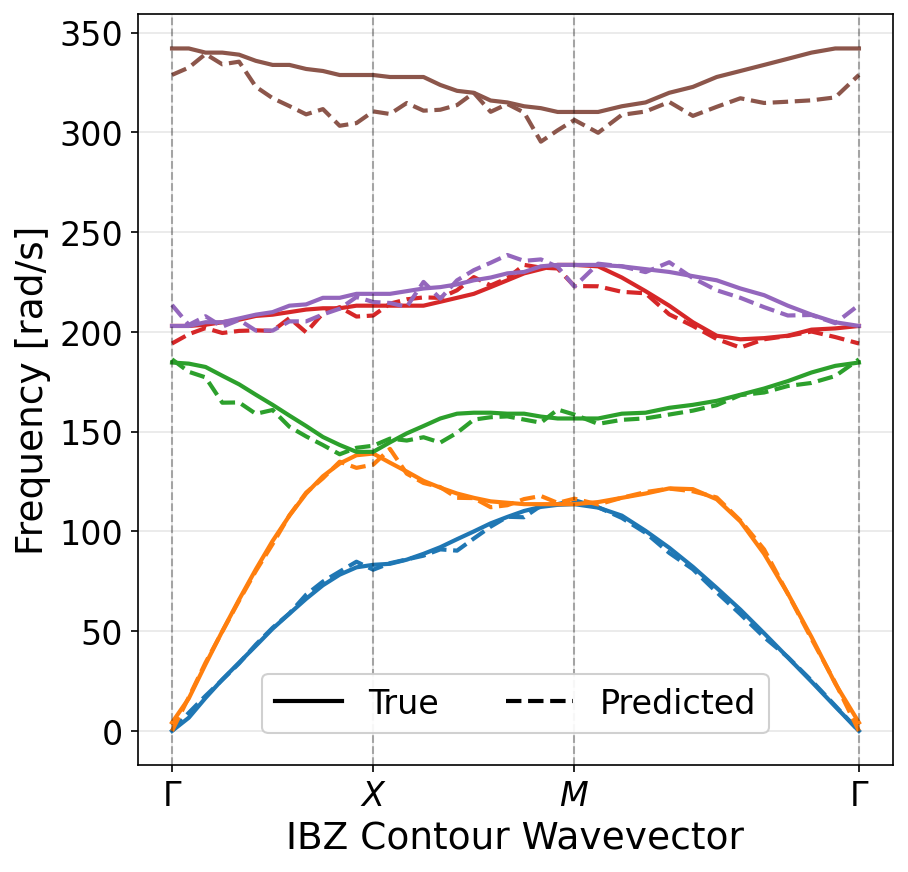
\includegraphics[width=\textwidth]{Figures/Dispersion B/NMAE252_NMSE328_g729.png}
        \caption{75th percentile performance.}
        \label{fig:dispersion_b_p75}
    \end{subfigure}
    \caption{Predicted and ground-truth dispersion bands for representative unseen discrete valued geometries spanning the 25th, 50th, and 75th percentiles of prediction performance.}
    \label{fig:dispersion_c_percentiles}
\end{figure}
Like with the continuous geometry figures, these plots represent the eigenfrequency predictions of the model across all 325 wavevectors forming the half plane for discrete valued geometries, downselected to be the horizontal, vertical, and diagonal traversal of the IBZ. Overall, the model performance is quite good at predictions in the encoded eigenfrequency, showing an average of $<1\%$ prediction error across all unseen samples.

\begin{figure}[H]
    \centering
    \begin{subfigure}[t]{0.49\textwidth}
        \centering
        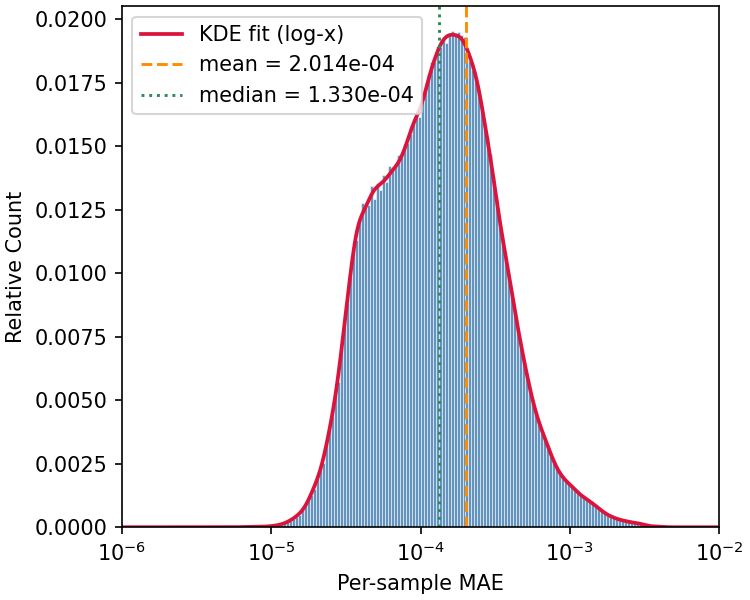
\includegraphics[width=\textwidth]{Figures/Statistics/freq_loss_histogram_mae_c_test.png}
        \caption{Performance histogram for continuous geometries.}
        \label{fig:freq_loss_histogram_continuous}
    \end{subfigure}
    \hfill
    \begin{subfigure}[t]{0.49\textwidth}
        \centering
        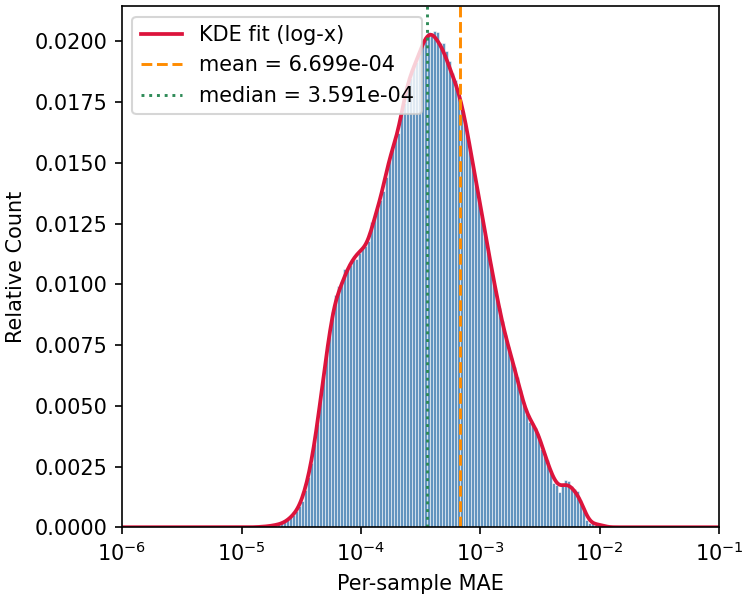
\includegraphics[width=\textwidth]{Figures/Statistics/freq_loss_histogram_mae_b_test.png}
        \caption{Performance histogram for discrete geometries.}
        \label{fig:freq_loss_histogram_discrete}
    \end{subfigure}
    \caption{Comparison of relative prediction error distributions for continuous-valued and discrete metamaterial geometries for the same model. While there are some tail outliers, most samples fall within the range of $~10^{-2}$ to $~10^{-4}$, indicating that the same model is able to learn continuous and discrete geometry cases.}
    \label{fig:freq_loss_histograms}
\end{figure}

%%%%%%%%%%%%%%%%%%%%%%%%%%%%%%%%%%%%%%%%%%%%%%%%%%%%%%%%%%%%%%%%%%%%%%
\subsection{Dependence of Prediction Error on Band and Boundary Length}
\label{ssec:boundary_length_vs_loss}

The preceding subsections showed that, although the same wavelet-conditioned FNO can predict displacement fields for both continuous and discrete unit cells, discrete geometries are systematically more difficult, with absolute and relative errors larger (Figures \ref{fig:disp_loss_histograms}, \ref{fig:freq_loss_histograms}), and the harder quartiles of the discrete test set degrading more visibly than their continuous counterparts. This gap is expected from the architecture of the FNO itself. Each Fourier layer retains only a truncated set of spectral modes after the discrete FFT. Smooth continuous material fields, and the comparatively smooth displacement modes they induce, concentrate their energy in a modest number of low-to-moderate wavenumbers and are therefore well represented by that truncated Fourier basis. Binary geometries, by contrast, contain jump discontinuities at material interfaces. Under an FFT, such discontinuities produce a broadband spectrum whose coefficients decay slowly with wavenumber, so a substantial fraction of the high-frequency content needed to resolve sharp phase boundaries lies outside the retained modes. The spectral branch therefore sees a degraded, band-limited version of the interface, yielding Gibbs-type ringing or blur and a harder operator-learning problem precisely when geometric discontinuity is more severe.
If this spectral-truncation explanation is correct, then even among discrete geometries the prediction error should increase with the boundary interface length. To test this empirically, we define the \emph{boundary length} of each binarized unit cell as the number of interior four-connected pixel edges separating a $0$-valued pixel from a $1$-valued pixel. This scalar is a discrete measure of interface complexity. For each of the $1000$ unseen discrete test geometries, we compute the mean absolute error (MAE) of the predicted displacement channels, averaged over all $325$ IBZ wavevectors, separately for each of the six retained eigenbands. The resulting relationships are shown in Figure~\ref{fig:boundary_vs_mae_by_band}.

\begin{figure}[H]
  \centering
  
\includegraphics[width=\textwidth]{Figures/Statistics/boundary_vs_mae_by_band_b_test.png}
  \caption{Mean displacement MAE versus interface boundary length, separated by color for each of the six eigenbands on the discrete test set. Points correspond to average performance on unit-cell geometries. Legend values $\rho$ are Spearman rank correlations. A positive trend appears for every band, consistent with degraded FNO accuracy as the total length of $0$/$1$ material interfaces increases.}
  \label{fig:boundary_vs_mae_by_band}
\end{figure}

Two complementary trends are apparent. First, for every band there is a positive monotonic association between boundary length and MAE, with Spearman correlations ranging from $\rho=0.644$ for band~$0$ to $\rho\approx0.42$--$0.56$ for the higher bands. Geometries with short interfaces are concentrated at lower absolute error, while geometries with long, meandering phase boundaries systematically occupy the upper portion of the cloud. This supports the interpretation that the hard cases for the learned operator are those for which the truncated Fourier representation must resolve more extensive sharp material transitions on the fixed $32\times32$ grid.
Second, absolute error itself increases with band index. Averaged over the test geometries, the mean wavevector-averaged MAE rises from approximately $1.6\times10^{-3}$ for band~$0$ to approximately $3.8\times10^{-3}$ for band~$5$. Higher bands correspond to more rapidly oscillating Bloch modes that concentrate energy nearer material interfaces and therefore inherit more of the geometric difficulty encoded by boundary length. Together with the continuous-versus-discrete comparisons above, Figure~\ref{fig:boundary_vs_mae_by_band} indicates that prediction difficulty on discrete designs is organized both by band (modal complexity) and by interface measure (geometric complexity), as expected when a spectral surrogate retains only a portion of the broadband Fourier content generated by discontinuities.

%%%%%%%%%%%%%%%%%%%%%%%%%%%%%%%%%%%%%%%%%%%%%%%%%%%%%%%%%%%%%%%%%%%%%%
\subsection{Band and Wavevector Encoding}
In solving this eigenvalue PDE with a FNO model, the first problem to solve was how to represent the constant parameters fed into the PDE. Specifically, for our PDE in equation \ref{eqn:eig_PDE}, we must specify the wavevectors, as well as which of the eigenvalue solutions (band) the model needs to solve. (The PDE has multiple eigenvalues and eigenvectors that satisfy it, corresponding to different deformation modes at different time frequencies.) Three encoding strategies were tried. The first is a constant-field representation, which can be considered the naive default option. In this representation, the two wavevectors $k_x$, $k_y$ and band $b$ are represented as $3 \times 32 \times 32$ images with constant pixel values, which would be stacked into a tensor and fed into the FNO. The problem with this approach is that the FNO model with this representation tends to experience mode collapse, being unable to learn anything, and outputting also constant field solutions. The reason for this is that a Fourier transform of a constant field would result in only one frequency (the constant frequency of 0) having a non-zero coefficient. Likewise, The resulting matrix from a fast Fourier transform (FFT) which is what is used in FNO, results in a matrix with all 0 values except for the center pixel which corresponds to the 0 frequency. This renders the frequency space branch of the Fourier layers shown in figure \ref{fig:FNO_architecture} effectively unable to contain or propagate information with this representation past the first layer. This in turn causes the Fourier branch to not be able to contribute at all to the model predictive power as it never contributes to any loss and thus cannot be trained. The remaining spatial domain branch of the FNO appears unable to handle the complexity of the problem. This is not surprising as it is essentially a standard CNN of shallow depth, which has not been shown in literature to be able to learn complex eigenvalue PDEs.

With this insight, the next embedding tried was a sinusoidal encoding, which does have unique representations that are not scaled versions of each other in the spectral domain. Here, we used a spatial domain sinusoid with the $x$ and $y$ frequencies a function of $b$ for the band encoding, and a function of $k_x$ and $k_y$ for the wavevector encodings. The resulting spatial domain encoding and its FFT are shown below.

% \begin{figure}[H]
%     \centering
%     \begin{subfigure}{\textwidth}
%         \centering
%         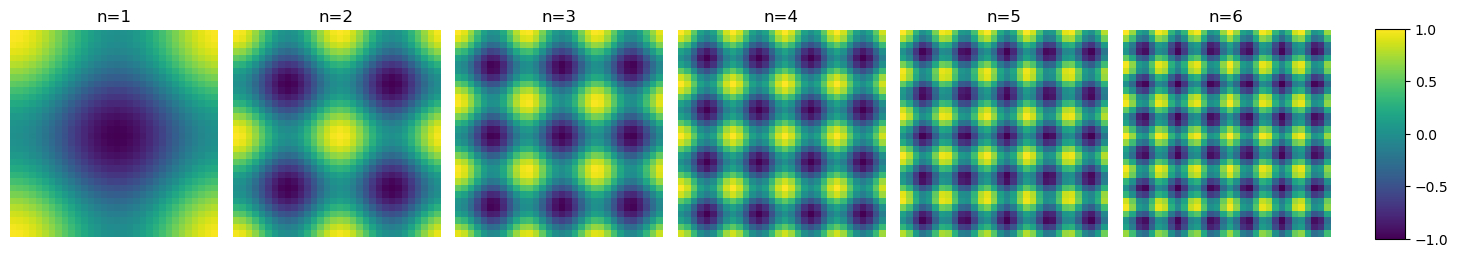
\includegraphics[width=\textwidth]{Figures/Methods/1D sinusoidal encoding.png}
%         \caption{The sinusoidal spatial encoding for band integer.}
%         \label{fig:1D_sinusoidal_encoding_spatial}
%     \end{subfigure}  
%     \begin{subfigure}{\textwidth}
%         \centering
%         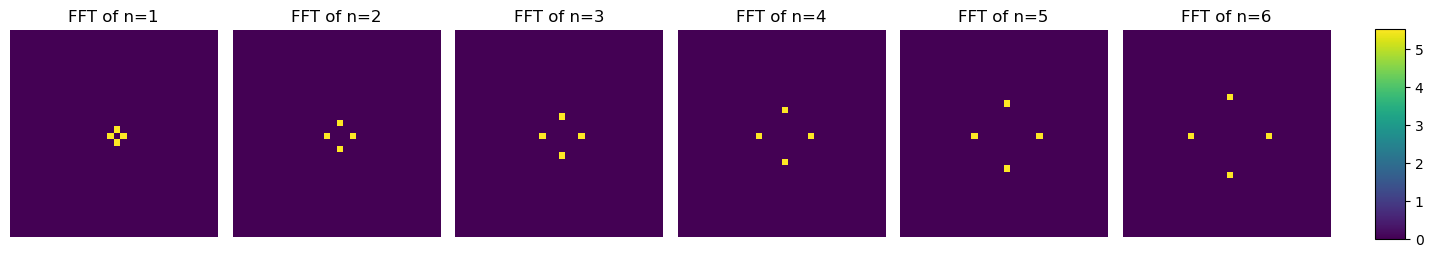
\includegraphics[width=\textwidth]{Figures/Methods/1D sinusoidal encoding fft.png}
%         \caption{The FFT of the above sinusoidal spatial encodings.}
%         \label{fig:1D_sinusoidal_encoding_fft}
%     \end{subfigure}
%     \caption{The sinusoidal encoding of the band integer (fig. \ref{fig:1D_sinusoidal_encoding_spatial}) and its FFT (fig. \ref{fig:1D_sinusoidal_encoding_fft}). 4 frequencies in the FFT show up as non-zero, corresponding to the +/- and x/y frequencies matching the encoded frequency. This encoding is intuitive, as visually one can count the peaks in the spatial domain to recover the band integer, and serves to carry information both in the spectral and in the spatial domains.}
%     \label{fig:1D_sinusoidal_encoding}
% \end{figure}

% \begin{figure}[H]
%     \centering
%     \begin{subfigure}{\textwidth}
%         \centering
%         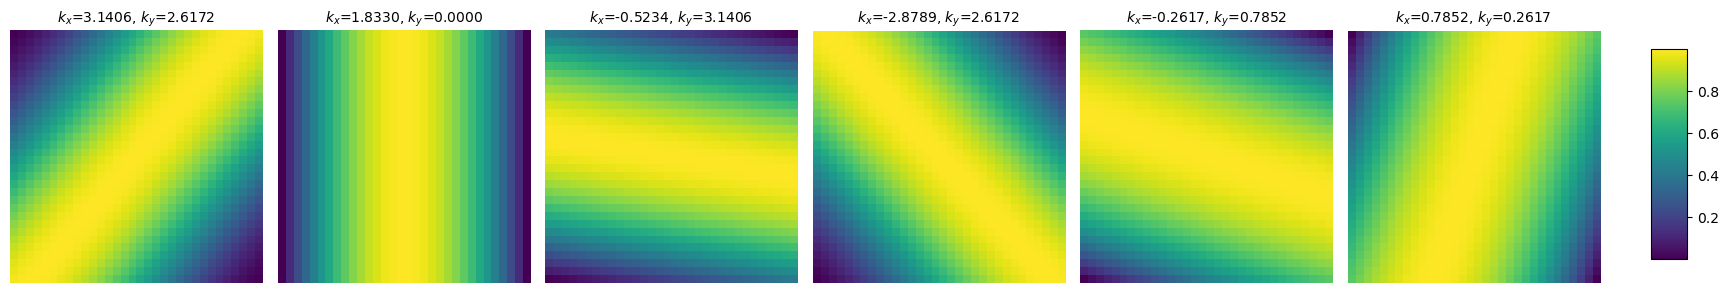
\includegraphics[width=\textwidth]{Figures/Methods/2D sinusoidal encoding.png}
%         \caption{The sinusoidal spatial encoding for $x$ and $y$ wavevectors.}
%         \label{fig:2D_sinusoidal_encoding_spatial}
%     \end{subfigure}  
%     \begin{subfigure}{\textwidth}
%         \centering
%         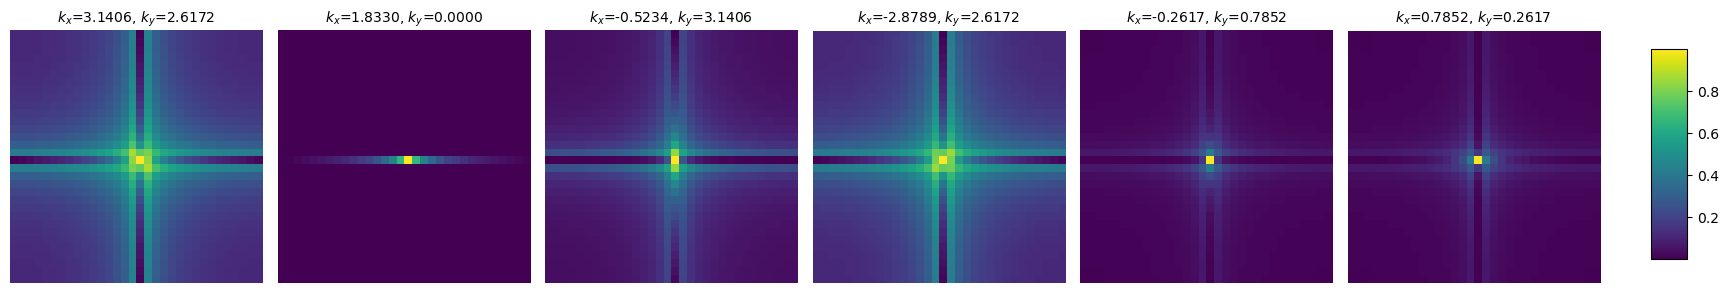
\includegraphics[width=\textwidth]{Figures/Methods/2D sinusoidal encoding fft.png}
%         \caption{The FFT of the above sinusoidal spatial encodings.}
%         \label{fig:2D_sinusoidal_encoding_fft}
%     \end{subfigure}
%     \caption{The sinusoidal encoding of the $x$ and $y$ wavevectors (\ref{fig:2D_sinusoidal_encoding_spatial}) and its FFT \ref{fig:2D_sinusoidal_encoding_fft}. The actual wavevectors are shown in the subplot titles. While the encoding is fairly intuitive as the $k_x$ and $k_y$ are scaled by $1/\pi$ and the resulting image is essentially what the waveform actually looks like physically. The FFT of many waveforms is similar in which pixels are non-zero, but different brightness for the +/-, x/y quadrants of the image, corresponding to a fairly intuitive image of the frequencies present. This similarity may not be a problem, as in general similar images can still be distinguished by CNN type models so long as there are sufficient differences, and an FNO architecture contains in one branch, the CNN architecture.}
%     \label{fig:2D_sinusoidal_encoding}
% \end{figure}

% With the sinusoidal encoding, the FNO model was able to learn fairly well the PDE problem, but tended to have a "fuzzy" structure where sharper edges would occur in the ground truth. See two random representative cases of unseen data inference showcasing the issue in figures \ref{fig:sinusoidal_s3} and \ref{fig:sinusoidal_s5} . At first, this was taken to be a symptom of underparameterization, as the model was grasping the problem in crude contours but could not learn the finer scale details well. 

% \begin{figure}[H]
%     \centering
%     \begin{subfigure}{0.48\textwidth}
%         \centering
%         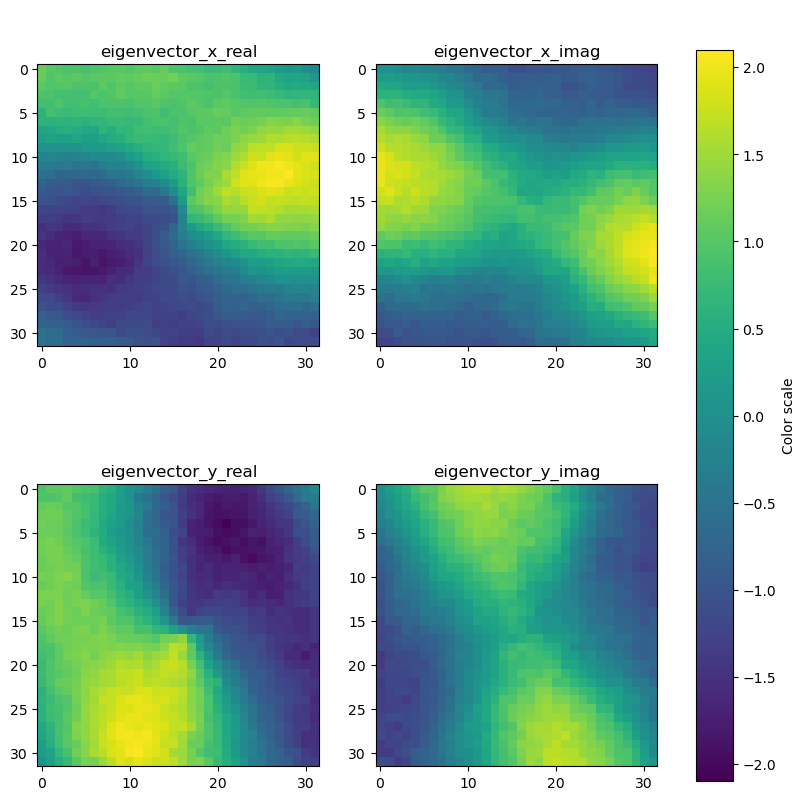
\includegraphics[width=\textwidth]{Figures/sinusoid/output_prediction3_hc64_lr1e-02_wd1e-02_ss10_gamma1e-01_e120_cropped.png}
%         \caption{FNO predictions}
%         \label{fig:sinusoidal_s3_prediction}
%     \end{subfigure}%
%     \hfill
%     \begin{subfigure}{0.48\textwidth}
%         \centering
%         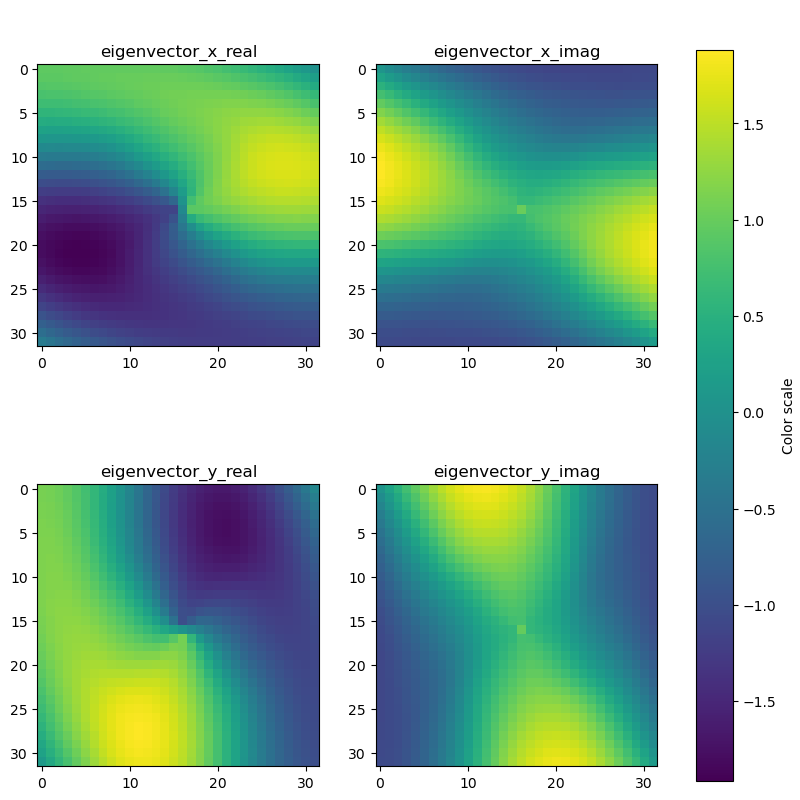
\includegraphics[width=\textwidth]{Figures/sinusoid/output_sample3_hc64_lr1e-02_wd1e-02_ss10_gamma1e-01_e120_cropped.png}
%         \caption{Ground truth}
%         \label{fig:sinusoidal_s3_truth}
%     \end{subfigure}%
%     \caption{The FNO predictions (left) and the ground truth FEA simulation (right) for a representative sample. The course structure is learned by the FNO, but the finer nuances are not grasped.}
%     \label{fig:sinusoidal_s3}
% \end{figure}

% \begin{figure}[H]
%     \centering
%     \begin{subfigure}{0.48\textwidth}
%         \centering
%         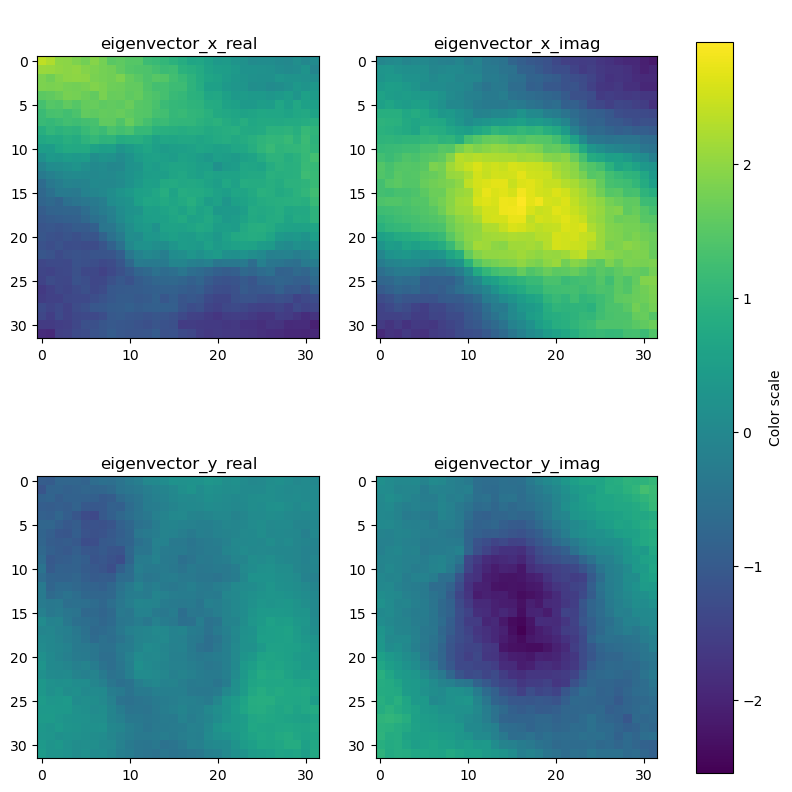
\includegraphics[width=\textwidth]{Figures/sinusoid/output_prediction5_hc64_lr1e-02_wd1e-02_ss10_gamma1e-01_e120_cropped.png}
%         \caption{FNO predictions}
%         \label{fig:sinusoidal_s5_prediction}
%     \end{subfigure}%
%     \hfill
%     \begin{subfigure}{0.48\textwidth}
%         \centering
%         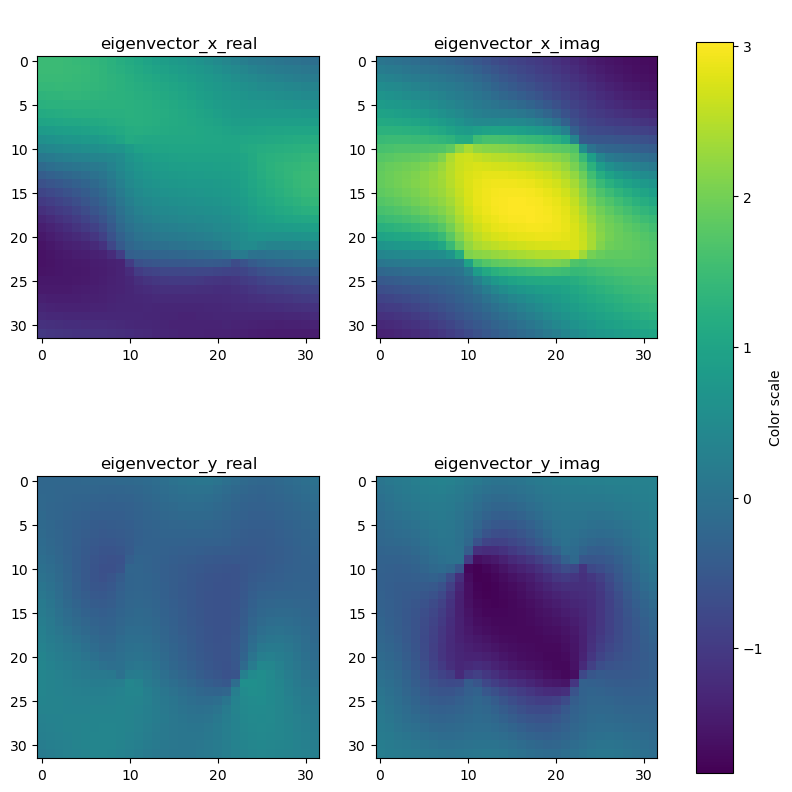
\includegraphics[width=\textwidth]{Figures/sinusoid/output_sample5_hc64_lr1e-02_wd1e-02_ss10_gamma1e-01_e120_cropped.png}
%         \caption{Ground truth}
%         \label{fig:sinusoidal_s5_truth}
%     \end{subfigure}%
%     \caption{The FNO predictions (left) and the ground truth FEA simulation (right) for another representative sample. The course structure is learned by the FNO, but the finer nuances are not grasped.}
%     \label{fig:sinusoidal_s5}
% \end{figure}

% Upon further investigation however by increasing the number of Fourier layers from 4 to 6, 8, and 10, and also increasing the number of hidden channels per layer from 64 to 128 and 256, it became clear the issue was not the number of parameters. The FNO representation of inputs past the first layer barely differed, which suggesting that some information was not being well propagated through the first layer, effectively leading to the same symptoms as underparameterization due to later layer parameters not playing much of a predictive role.

% It was hypothesized that although the sinusoidal encodings lead to unique and meaningful representations in both the spatial and spectral domains, the sparsity of the spectral domain matrix meant that the Fourier branch of the FNO was still not playing much of a role, and an encoding where the Fourier branch of the FNO was richly interacting with the input data would likely perform better. From this, the custom wavelet encoding schema described in section \ref{sec:Methodology} was developed. See figures \ref{fig:1D_wavelet_encoding} and \ref{fig:2D_wavelet_encoding} for examples of band and wavevectors representations under the wavelet encoding.

% \begin{figure}[H]
%     \centering
%     \begin{subfigure}{\textwidth}
%         \centering
%         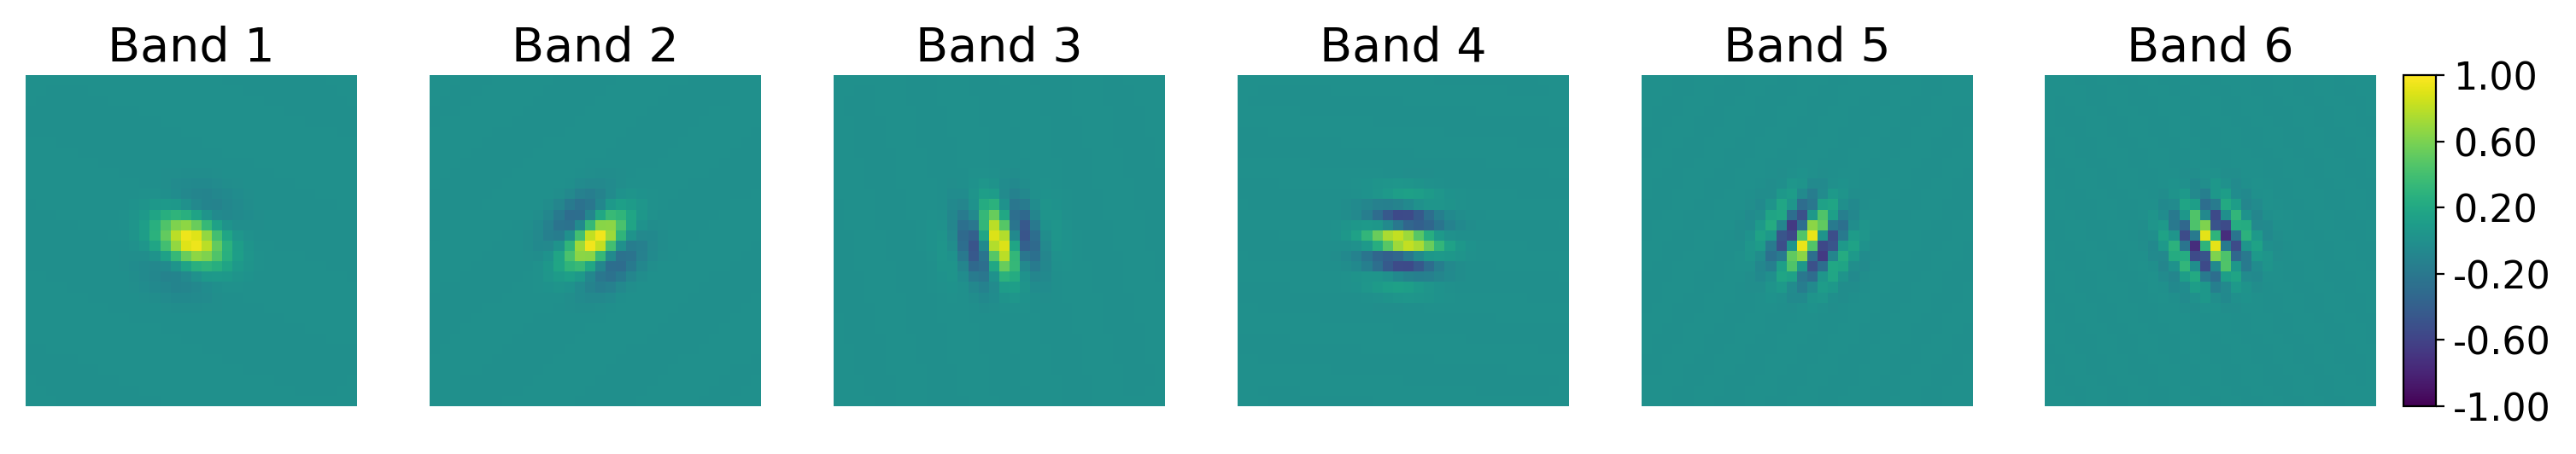
\includegraphics[width=\textwidth]{Figures/Methods/1D wavelet encoding.png}
%         \caption{The wavelet spatial encoding for band integer.}
%         \label{fig:1D_wavelet_encoding_spatial}
%     \end{subfigure}  
%     \begin{subfigure}{\textwidth}
%         \centering
%         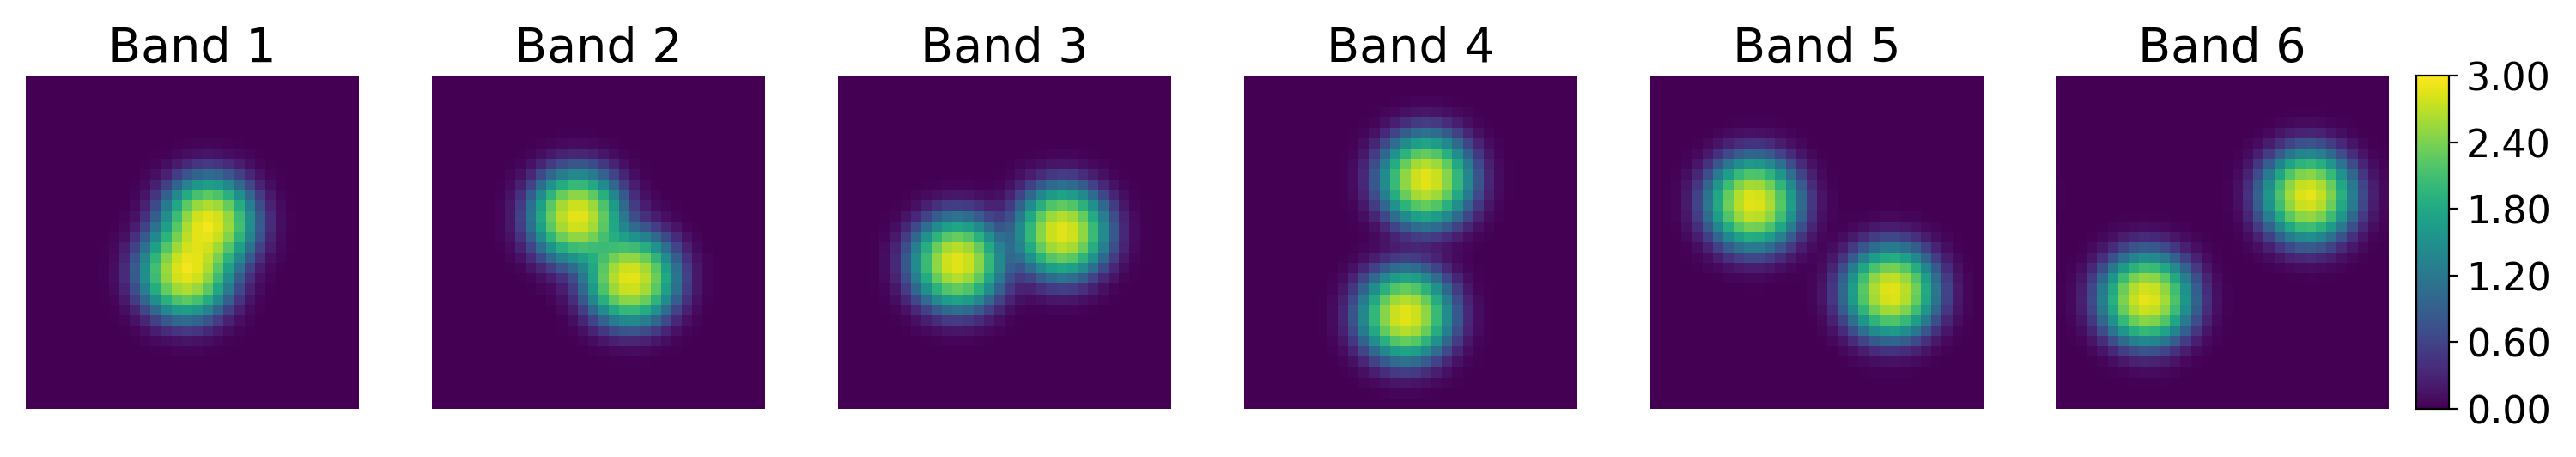
\includegraphics[width=\textwidth]{Figures/Methods/1D wavelet encoding fft.png}
%         \caption{The FFT of the above wavelet spatial encodings.}
%         \label{fig:1D_wavelet_encoding_fft}
%     \end{subfigure}
%     \caption{The wavelet encoding of the band integer (fig. \ref{fig:1D_wavelet_encoding_spatial}) and its FFT (fig. \ref{fig:1D_wavelet_encoding_fft}). Each band corresponds to a unique wavelet with representation in both spatial and spectral domains. Compared with the sinusoidal embeddings in fig. \ref{fig:1D_sinusoidal_encoding_spatial} and \ref{fig:1D_sinusoidal_encoding_fft}, the information distribution is also much more balanced between the two domains, with much more of the spectral domain pixels being utilized for each case. This in turn allows for both greater discernibility and richer interactions between the FNO weights and the band parameter input.}
%     \label{fig:1D_wavelet_encoding}
% \end{figure}

% \begin{figure}[H]
%     \centering
%     \begin{subfigure}{\textwidth}
%         \centering
%         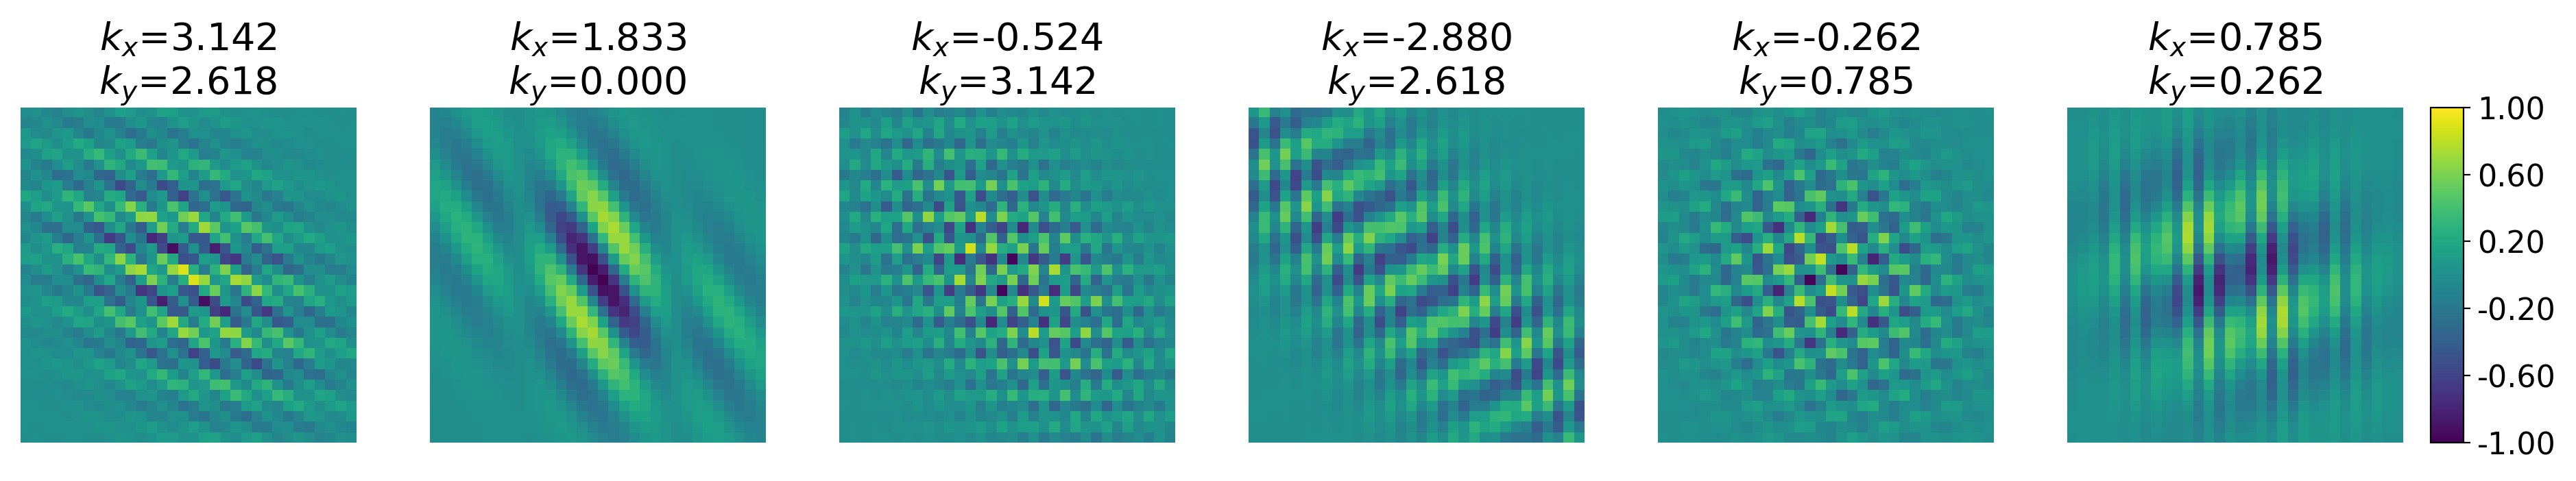
\includegraphics[width=\textwidth]{Figures/Methods/2D wavelet encoding.png}
%         \caption{The wavelet spatial encoding for $x$ and $y$ wavevectors.}
%         \label{fig:2D_wavelet_encoding_spatial}
%     \end{subfigure}  
%     \begin{subfigure}{\textwidth}
%         \centering
%         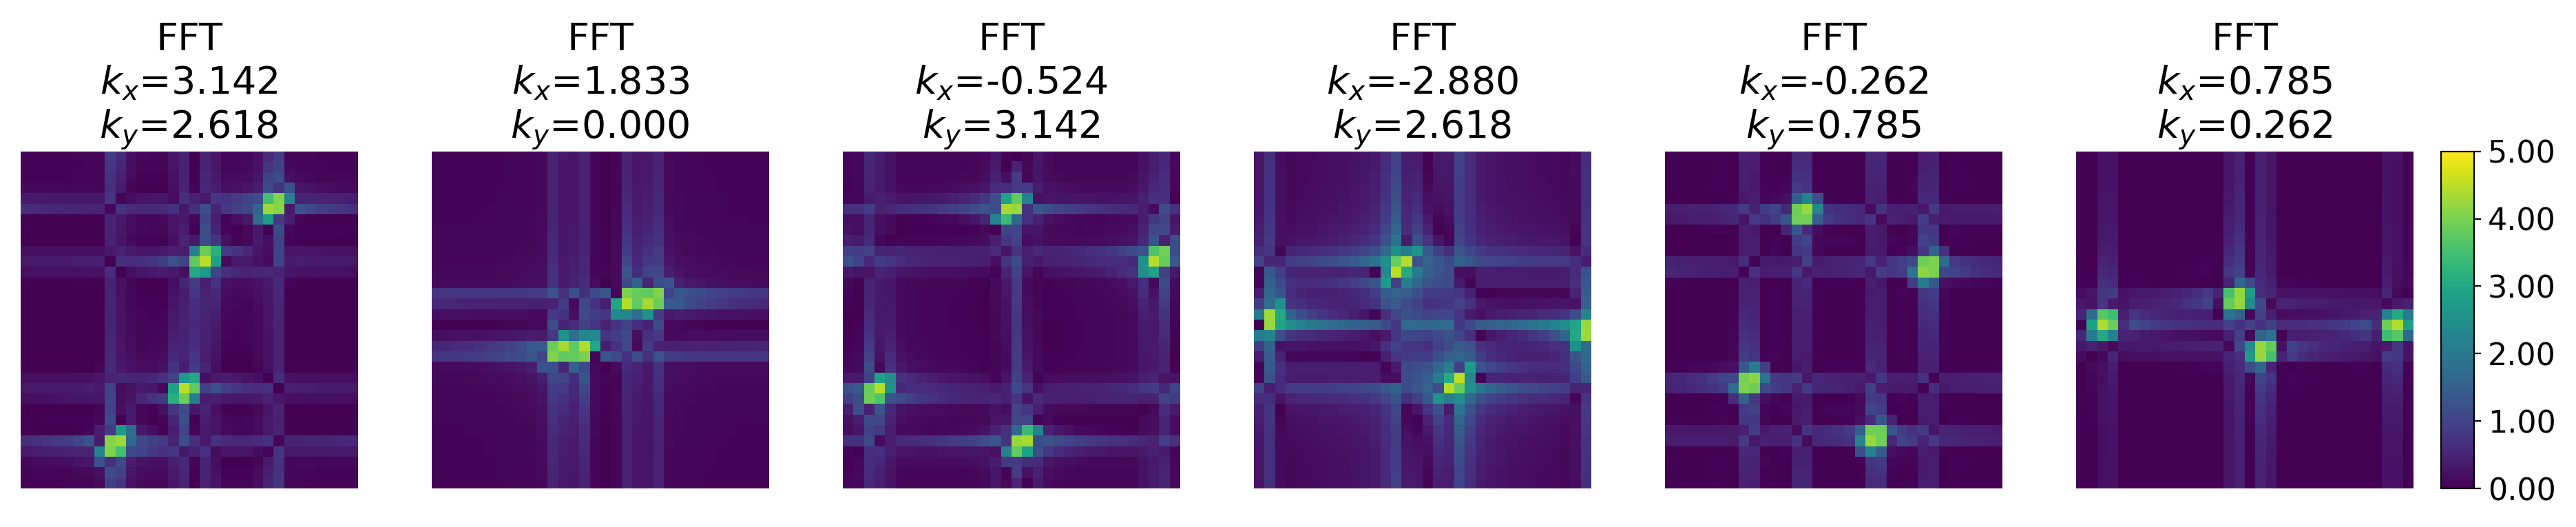
\includegraphics[width=\textwidth]{Figures/Methods/2D wavelet encoding fft.png}
%         \caption{The FFT of the above wavelet spatial encodings.}
%         \label{fig:2D_wavelet_encoding_fft}
%     \end{subfigure}
%     \caption{The wavelet encoding of the $x$ and $y$ wavevectors (\ref{fig:2D_wavelet_encoding_spatial}) and its FFT \ref{fig:2D_wavelet_encoding_fft}. The actual wavevectors are shown in the subplot titles. For each $k_x$ and $k_y$ value pair, there is a unique mapping in both the spatial and spectral domain representations. Compared with the sinusoidal embeddings in fig. \ref{fig:2D_sinusoidal_encoding_spatial} and \ref{fig:2D_sinusoidal_encoding_fft}, the wavelet embedding has less pixel overlap and utilizes much more of the pixel space for different $k_x$ and $k_y$ values which leads to greater differentiation and thus more possible and more orthogonal interactions between the FNO weights in both branches and the input.}
%     \label{fig:2D_wavelet_encoding}
% \end{figure}

% The encoding proved to be substantially more effective for the model's learning outcomes, for all tried combinations of model and training hyperparameters. See figures \ref{fig:wavelet_s1} and \ref{fig:wavelet_s2} for random representative samples of model performance using the wavelet encoding for band and wavevectors.

% \begin{figure}[H]
%     \centering
%     \begin{subfigure}{0.8\textwidth}
%         \centering
%         
\includegraphics[width=\textwidth]{Figures/input2.png}
%         \caption{Random sample inputs}
%         \label{fig:wavelet_s1_input}
%     \end{subfigure}%
%     \hfill
%     \begin{subfigure}{\textwidth}
%         \centering
%         
\includegraphics[width=\textwidth]{Figures/output2.png}
%         \caption{Random sample outputs, targets, and differences}
%         \label{fig:wavelet_s1_output}
%     \end{subfigure}%
%     \caption{Performance of the FNO model with wavelet embedding on unencountered geometries. Inputs are shown in fig. \ref{fig:wavelet_s1_input} and outputs, targets, and differences are shown in fig. \ref{fig:wavelet_s1_output}}
%     \label{fig:wavelet_s1}
% \end{figure}

% \begin{figure}[H]
%     \centering
%     \begin{subfigure}{0.8\textwidth}
%         \centering
%         
\includegraphics[width=\textwidth]{Figures/input4.png}
%         \caption{Random sample inputs}
%         \label{fig:wavelet_s2_inputs}
%     \end{subfigure}%
%     \hfill
%     \begin{subfigure}{\textwidth}
%         \centering
%         
\includegraphics[width=\textwidth]{Figures/output4.png}
%         \caption{Random sample outputs, targets, and differences}
%         \label{fig:wavelet_s2_outputs}
%     \end{subfigure}%
%     \caption{Performance of the FNO model with wavelet embedding on unencountered geometries. Inputs are shown in fig. \ref{fig:wavelet_s2_input} and outputs, targets, and differences are shown in fig. \ref{fig:wavelet_s2_output}}
%     \label{fig:wavelet_s2}
% \end{figure}

\subsection{Output Datatype}
\label{ssec:output_datatype}
The natural representation of the output data is a complex field for both x and y displacements. However, it was found that the models trained on a $2\times 32 \times 32$ complex64 tensor representation did not perform statistically significantly differently compared with a $4\times 32 \times 32$ float16 tensor representation across any hyperparameter setting. In both cases, it takes within 20 epochs for training to converge, and final accuracies evaluated on an unseen test set are within 10\% relative difference for all combinations of hyperparameters. There is only one major difference between the two cases, which is that the complex64 case consistently takes $1.5$ to $2 \times$ longer to train, which is a notable disadvantage. If there was a complex32 data format in Python, it might be competitive against float16, but in its absence, even for a naturally complex tensor, we recommend float16 as the training datatype unless higher precision is absolutely necessary. 

\section{Conclusions}
\label{sec:Conclusion}
In this work, we have demonstrated that Fourier Neural Operators, when combined with structured wavelet encodings of PDE parameters, can serve as efficient and accurate surrogates for eigenvalue PDE solvers, allowing for user toggling between the different solutions deterministically and repeatably by choice of PDE parameters in inputs. The specific example is of a non-trivial 2D PDE based on acoustic wave propagation through metamaterial geometries. It is evident from this work that the choice of embedding when using neural networks or neural operators that have specific transforms built into its architecture should be matched to the transforms. In this particular case, the FNO is actually somewhat of a misnomer, because it contains both a spatial and spectral learned kernel interacting with a spatial and spectral representation of the layer input. In this sense, it is more like a Wavelet Neural Operator. Because of this spatial and frequency domain duality and the FNO simultaneously computing and learning in both domains, wavelet embeddings which preserve both spatial and frequency domain information outperform embeddings which only use one of the two domains.

The ability for FNOs paired with wavelet encodings to solve eigenvalue PDEs and generalize well past its training geometries to novel geometries, opens up many opportunities in the metamaterial research field directly, but also many other fields of computational mechanics and physics that also have their own eigenvalue PDEs with input parameters that toggle between different solutions. This model, at 2 GB of size with float16 precision, is very lightweight compared to enterprise FEA software and processes inputs on the order of milliseconds, making it a compelling tool for surrogate modeling and/or iterative design for myriad materials and structure engineering problems. Future work to expand on usability could include generalization tests to different resolutions, using physics informed losses to further enhance performance and/or generalizability, and allowing more parameters such as material constants to be used as toggles for solutions, expanding the problem and solution space to more dimensions.

\section*{AI Usage Disclosure}
\todo{Add disclosure for how AI was used in this project}

\section*{Declaration of Competing Interest}
The authors declare that they have no known competing financial interests or personal relationships that could have appeared to influence the work reported in this paper.

\section*{CRediT authorship contribution statement}


\section*{Data availability}
\label{sec:Repository}
The code and data in this article can be found at this GitHub repository:
\url{https://github.com/trutheresy/NO-2D-Metamaterials}.

The code for FEA computations can be found at this GitHub Repository:
\url{https://github.com/aco8ogren/2D-dispersion.git}.

\section*{Acknowledgements}

%% If you have bibdatabase file and want bibtex to generate the
%% bibitems, please use
%%
\bibliographystyle{elsarticle-num}
%\bibliographystyle{plain} 
\bibliography{references}
%%\begin{thebibliography}{00}
%% \bibitem[Author(year)]{label}
%%\end{thebibliography}

\clearpage
\appendix

\renewcommand{\thesection}{S\arabic{section}}
\renewcommand{\thesubsection}{S\arabic{section}.\arabic{subsection}}
\renewcommand{\thefigure}{S\arabic{figure}}
\renewcommand{\thetable}{S\arabic{table}}
\renewcommand{\theequation}{S\arabic{equation}}

\setcounter{figure}{0}
\setcounter{table}{0}
\setcounter{equation}{0}

\section{Supplementary Information}
\label{sec:supplement}
\subsection{Model and Training Hyperparameters}
\begin{table}[H]
    \centering
    \begin{tabular}{|c|c|c|c|c|}
        \hline
        \textbf{Hyperparameter} &
        \multicolumn{4}{c|}{\textbf{Candidate Settings}} \\ \hline
    
        \textbf{Fourier Layers} & \textit{4} & 6 & 8 & 12 \\ \hline
        \textbf{Hidden Channels} & 32 & 64 & \textit{128} & 256 \\ \hline
        \textbf{Activation Function} & ReLU & \textit{GELU} & tanh & Sigmoid \\ \hline
        \textbf{Loss Criterion} & L1 & L2 & \textit{Huber} & SSIM \\ \hline
        \textbf{Epochs} & 8 & \textit{12} & 16 & 20 \\ \hline
        \textbf{Learning Rate} & $10^{-4}$ & \textit{$10^{-3}$} & $10^{-2}$ & $10^{-1}$ \\ \hline
        \textbf{Weight Decay} & 0 & \textit{$10^{-4}$} & $10^{-3}$ & $10^{-2}$ \\ \hline
        \textbf{Gamma} & 0 & 0.01 & \textit{0.1} & 0.5 \\ \hline
        \textbf{Step Size} & 0 & 1 & \textit{4} & 10 \\ \hline
        \textbf{Batch Size} & 64 & 128 & 256 & \textit{512} \\ \hline
        \textbf{Data Precision} & F8 E4M3 & F8 E5M2 & \textit{F16} & F32 \\ \hline
    \end{tabular}
    \caption{Combinations tried in grid search for optimal model and training hyperparameters.}
    \label{tab:training_hyperparameters}
\end{table}

\subsection{Loss Criterion}
In the exploration of optimal training protocols for the FNO model, other loss functions were trialed as training criterion: mean absolute error (MAE), mean squared error (MSE), normalized MAE, normalized MSE, Huber (smooth L1), and structural similarity index (SSI). For purposes of comparison, the validation criterion was chosen to be MAE and MSE. Broadly speaking, models that performed the best in terms of MSE also performed the best in MAE. The training criterion that yielded the lowest MAE and MSE loss was the Huber loss. All criterion followed a learning rate of $2\times10^{-3}$ with a decay factor per epoch of $0.9$. The mathematical definitions for each area as follows. Losses were evaluated and aggregated across all 5 output channels. 

\begin{itemize}
    \item The mean absolute error (MAE) loss is defined as
\begin{equation*}
    \mathcal{L}_{\text{MAE}} = \frac{1}{HW} \sum_{i=0}^{H-1} \sum_{j=0}^{W-1} \sum_{c=0}^{4} \left| \hat{u}_{c}(i,j) - u_{c}(i,j) \right|
\end{equation*}

Experimentally, models trained exclusively with MAE produced predictions with sharper interfaces and better-preserved boundary features than those trained solely with MSE. This behavior is consistent with the linear penalty of MAE, which does not disproportionately penalize isolated large residuals near discontinuities. Despite the improved qualitative sharpness, MAE training converged to higher validation MAE and MSE than Huber loss, indicating that the improved preservation of fine structural features came at the expense of overall numerical accuracy. This observation also motivated the hybrid training schedule in which optimization began with MAE before transitioning to MSE, combining the edge-preserving characteristics of MAE with the stronger refinement of large residuals provided by MSE.

\item The mean squared error (MSE) loss is defined as
\begin{equation*}
    \mathcal{L}_{\text{MSE}} = \frac{1}{HW} \sum_{i=0}^{H-1} \sum_{j=0}^{W-1} \sum_{c=0}^{4} \left( \hat{u}_{c}(i,j) - u_{c}(i,j) \right)^2
\end{equation*}

The quadratic penalty of MSE assigns increasingly large gradients to larger residuals, causing the optimizer to preferentially reduce regions with the greatest numerical error. As a consequence, the loss favors smooth predictions that minimize the overall energy of the residual rather than preserving sharp transitions. Experimentally, models trained exclusively with MSE produced outputs that reproduced the correct magnitude and large-scale structure of the solution, but exhibited diffuse interfaces and blurred boundaries. Fine-scale features were often replaced by low-amplitude, grainy artifacts, consistent with the tendency of MSE to average over uncertain or discontinuous regions in order to minimize the global squared error.

\item A hybrid MAE--MSE training schedule was also evaluated, where the model was optimized using MAE for the first half of the training epochs before switching to MSE for the remaining half. This training strategy approximates the behavior of the Huber loss over the course of optimization. During the early stages of training, prediction errors are typically large, making the linear penalty of MAE advantageous for preserving sharp interfaces while preventing large residuals from dominating the optimization. As training progresses and the average residual decreases, switching to MSE increases the emphasis on refining the remaining prediction errors and improving overall numerical accuracy.

Experimentally, this training schedule consistently outperformed training with either MAE or MSE alone for the same total number of epochs. The resulting predictions retained substantially sharper boundaries than models trained exclusively with MSE, while achieving lower validation MAE and MSE than models trained exclusively with MAE. Among the non-Huber training strategies investigated, the hybrid schedule produced the best overall balance between qualitative feature preservation and quantitative accuracy, converging to within approximately 10\% of the validation error achieved by Huber loss. Although less adaptive than Huber, which transitions between MAE- and MSE-like behavior on a per-residual basis, the epoch-wise transition captures much of the same optimization benefit.

\item The structural similarity index measure (SSIM) is defined as

\begin{equation*}
\mathcal{L}_{\text{SSIM}}
=
1
-
\frac{1}{5}
\sum_{c=0}^{4}
\frac{
\left(2\mu_{u_c}\mu_{\hat{u}_c}+C_1\right)
\left(2\sigma_{u_c\hat{u}_c}+C_2\right)
}{
\left(\mu_{u_c}^2+\mu_{\hat{u}_c}^2+C_1\right)
\left(\sigma_{u_c}^2+\sigma_{\hat{u}_c}^2+C_2\right) 
}, \quad \text{where}
\end{equation*}
\begin{equation*}
\mu_{u_c}
=
\frac{1}{HW}
\sum_{i=0}^{H-1}
\sum_{j=0}^{W-1}
u_c(i,j), \quad 
\sigma_{u_c\hat{u}_c}
=
\frac{1}{HW}
\sum_{i=0}^{H-1}
\sum_{j=0}^{W-1}
\left(u_c(i,j)-\mu_{u_c}\right)
\left(\hat{u}_c(i,j)-\mu_{\hat{u}_c}\right)
\end{equation*}

A significant limitation of SSIM arises when it is applied to signed-valued fields. Unlike its original application to nonnegative image intensities, a perfect sign-reversed field ($\hat{u}=-u$) can achieve nearly the same SSIM score as a perfect reconstruction ($\hat{u}=u$). Consequently, a model trained solely with SSIM may converge to physically incorrect solutions containing polarity inversions while still minimizing the loss. The following derivation demonstrates the mathematical origin of this ambiguity.

For the purposes of the following discussion, we consider the common case where the stabilizing constants satisfy
\begin{equation*}
    C_1 \ll 2\mu_{u_c}^2,
    \qquad
    C_2 \ll 2\sigma_{u_c}^2,
\end{equation*}
allowing them to be neglected.

For a correct reconstruction,
\begin{equation*}
    u_c^{(+)} = u_c,
\end{equation*}
the SSIM score is
\begin{equation*}
\mathrm{SSIM}(u_c,u_c^{(+)})
=
\frac{\left(2\mu_{u_c}^2\right)\left(2\sigma_{u_c}^2\right)}
{\left(2\mu_{u_c}^2\right)\left(2\sigma_{u_c}^2\right)}
=1.
\end{equation*}

Now consider a sign-reversed reconstruction,
\begin{equation*}
    u_c^{(-)}=-u_c.
\end{equation*}
The mean reverses sign,
\begin{equation*}
    \mu_{u_c^{(-)}}=-\mu_{u_c},
\end{equation*}
the covariance likewise reverses sign,
\begin{equation*}
    \sigma_{u_c,u_c^{(-)}}
    =
    -\sigma_{u_c,u_c},
\end{equation*}
while the variance is unchanged,
\begin{equation*}
    \sigma_{u_c^{(-)}}^2=\sigma_{u_c}^2.
\end{equation*}
Substituting these relationships into the SSIM expression gives
\begin{equation*}
\mathrm{SSIM}(u_c,u_c^{(-)})
=
\frac{\left(-2\mu_{u_c}^2\right)\left(-2\sigma_{u_c}^2\right)}
{\left(2\mu_{u_c}^2\right)\left(2\sigma_{u_c}^2\right)}=1.
\end{equation*}
The numerator therefore differs from that of a correct reconstruction by two factors of $-1$, and thus, under these conditions, SSIM assigns essentially the same similarity score to a field and its sign-reversed counterpart as it does to a perfect reconstruction. This ambiguity constitutes a significant limitation when SSIM is applied to signed-valued regression problems where the polarity of the solution is physically meaningful. During training, the network frequently converged to predictions in which localized regions or the entire image were the negative of the correct solution while still achieving a favorable SSIM objective. Although the resulting fields exhibited accurate interface locations, boundary geometry, and overall morphology, the polarity inversions rendered the predictions physically incorrect. Consequently, SSIM should not be used as the sole training criterion for signed-valued fields unless it is supplemented by an additional loss that explicitly penalizes sign reversals.

\item The normalized mean absolute error (NMAE) loss is defined as
\begin{equation*}
    \mathcal{L}_{\text{NMAE}} = \frac{1}{HW} \sum_{i=0}^{H-1} \sum_{j=0}^{W-1} \sum_{c=0}^{4} \frac{\displaystyle \left| \hat{u}_{c}(i,j) - u_{c}(i,j) \right|}{\left| u_{c}(i,j) \right| + \varepsilon}
\end{equation*}
Unlike MAE, NMAE weights each prediction error by the inverse magnitude of the target value, causing the optimization to place greater emphasis on regions where the ground-truth solution is small in scale. Consequently, the loss seeks to minimize relative error rather than absolute error, preventing low-magnitude features from being dominated by high-magnitude regions during training.

Experimentally, NMAE successfully reduced the relative error in low-amplitude portions of the solution. However, this improvement came at the expense of increased overall MAE and MSE compared with training using the standard MAE loss. For the present application, the absolute magnitude of the prediction error was determined to be of greater practical importance than the relative error. As a result, the improved accuracy in low-valued regions did not outweigh the degradation in overall numerical accuracy, making NMAE a less suitable optimization criterion for the objectives of this work. However, for other applications, NMAE can be a valid and superior training criterion than standard MAE.

\item The normalized mean squared error (NMSE) loss is defined as
\begin{equation*}
    \mathcal{L}_{\text{NMSE}} = \frac{1}{HW} \sum_{i=0}^{H-1} \sum_{j=0}^{W-1} \sum_{c=0}^{4} \frac{\displaystyle \left(\hat{u}_{c}(i,j) - u_{c}(i,j) \right)^2}{\left( u_{c}(i,j) \right)^2 + \varepsilon}
\end{equation*}

Similar to NMAE, NMSE normalizes the prediction error by the magnitude of the target field, causing the optimization to prioritize relative error rather than absolute error. The quadratic penalty retains the characteristic behavior of MSE by assigning greater weight to larger residuals, while the normalization emphasizes regions where the target magnitude is small.

Experimentally, NMSE reduced the relative error in low-amplitude regions compared with standard MSE. However, this improvement was accompanied by increased overall validation MAE and MSE, performing worse than conventional MSE optimization. As with NMAE, the objective of this work was to minimize the absolute prediction error rather than the relative error. Consequently, the increased emphasis placed on low-magnitude regions did not translate into improved overall predictive performance, making NMSE less appropriate for the present application.
\end{itemize}

\subsection{Output Wavelet Encoding}
\label{ssec:output_wavelet_encoding}
Unlike with the input wavelets encodings which we already know all the possible decoded quantities, model outputs can fall anywhere within a range of valid values. There are two types of output fields. One is a displacement field, which is directly represented as its raw displacement values and requires no encoding. Four of the five output channels contain this type of information (real and imaginary x and y displacements). The fifth channel however, representing eigenfrequency, carries the same issue as wavevector and band of being a scalar valued quantity by nature. For this quantity, we need a way to encode into a wavelet form that the model can train on effectively and decode back to a numerical representation subsequently.
\begin{figure}[H]
  \centering
  
\includegraphics[width=\textwidth]{Figures/Methods/eigenfrequency_encoding.png}
  \caption{Log scale spaced examples of encoded frequencies from a min of 1Hz to a max of 8000Hz}
  \label{fig:eigenfrequency_encoding}
\end{figure}

\begin{figure}[H]
  \centering
  
\includegraphics[width=\textwidth]{Figures/Methods/eigenvalue_encode_decode_error_test.png}
  \caption{Decoding error of encoded frequencies from a min of 1Hz to a max of 8000Hz}
  \label{fig:eigenfrequency_encoding}
\end{figure}

\subsection{Algorithms for Gabor Wavelet Encoding}
This encoding strategy is used for mapping band integers to a 2D wavelet image.
\begin{algorithm}[H]
\caption{1D Gabor Wavelet Embedding from Scalar Input}
\label{alg:1d_gabor_embedding}
\begin{algorithmic}[1]
\STATE \textbf{INPUT:} Integer \( b \); grid size \( S \leftarrow 32 \); frequency scale \( r \leftarrow 2.0 \)
\STATE Create linspace vectors \( x, y \in [-1, 1] \) with \( S \) points
\STATE Construct meshgrid \( X, Y \leftarrow \text{meshgrid}(x, y) \)
\STATE Compute base frequency:
\[
f \leftarrow (1.0 + |b|) \cdot \frac{S}{8}
\]
\STATE Compute rotation angle:
\[
\theta \leftarrow (b \bmod 8) \cdot \frac{S}{16}
\]
\STATE Rotate coordinates:
\[
X_\theta \leftarrow X \cos \theta + Y \sin \theta, \quad
Y_\theta \leftarrow -X \sin \theta + Y \cos \theta
\]
\STATE Set Gaussian envelope widths:
\[
\sigma_x \leftarrow \sigma_y \leftarrow \frac{0.3}{r}
\]
\STATE Compute Gabor wavelet embedding:
\[
\psi_b(x, y) \leftarrow
\exp\left(-\frac{X_\theta^2}{2 \sigma_x^2} - \frac{Y_\theta^2}{2 \sigma_y^2}\right)
\cdot \cos(f \cdot X_\theta)
\]
\STATE \textbf{RETURN:} \( \psi_b \in \mathbb{R}^{S \times S} \)
\end{algorithmic}
\end{algorithm}

In Algorithm \ref{alg:1d_gabor_embedding}, a grid size of 32 is used so that the image size matches that of the geometry, for ease of ingestion of the FNO model. The base frequency is set to 8, which allows for up to the first 8 bands to be encoded as unique rotations and wavelet spatial frequencies in the domain. The frequency scale $r$ and constants such as 16 and 0.3 were picked so that the images utilized most of the domain and showed sufficient scale variation across the domain.

\begin{algorithm}[H]
\caption{2D Gabor Wavelet Embedding for Wavevectors}
\label{alg:2d_gabor_embedding}
\begin{algorithmic}[1]
\STATE \textbf{INPUT:} Integers \( k_x, k_y \); grid size \( S \leftarrow 32 \); frequency scale \( r \leftarrow 1.0 \)
\STATE Create linspace vectors \( x, y \in [-1, 1] \) with \( S \) points
\STATE Construct meshgrid \( X, Y \leftarrow \text{meshgrid}(x, y) \)
\STATE Compute frequencies:
\[
f_x \leftarrow (1.01 + k_x) \cdot \frac{S}{2}, \quad f_y \leftarrow (1.01 + k_y) \cdot \frac{S}{2}
\]
\STATE Compute rotation angles:
\[
\theta_x \leftarrow (k_x \bmod 5) \cdot \frac{\pi}{5}, \quad \theta_y \leftarrow (k_y \bmod 7) \cdot \frac{\pi}{7}
\]
\STATE Rotate coordinates:
\[
X_\theta \leftarrow X \cos \theta_x + Y \sin \theta_y, \quad
Y_\theta \leftarrow -X \sin \theta_x + Y \cos \theta_y
\]
\STATE Set Gaussian envelope widths:
\[
\sigma_x \leftarrow \sigma_y \leftarrow \frac{0.4}{r}
\]
\STATE Compute Gabor wavelet embedding:
\[
\psi_{k_x, k_y}(x, y) \leftarrow
\exp\left(-\frac{X_\theta^2}{2 \sigma_x^2} - \frac{Y_\theta^2}{2 \sigma_y^2}\right)
\cdot \sin(f_x X_\theta) \cdot \sin(f_y Y_\theta)
\]
\STATE \textbf{RETURN:} \( \psi_{k_x, k_y} \in \mathbb{R}^{S \times S} \)
\end{algorithmic}
\end{algorithm}

Like with Algorithm \ref{alg:1d_gabor_embedding}, in Algorithm \ref{alg:2d_gabor_embedding}, a grid size of 32 is used for FNO model ease of ingestion. The wavevectors are used to compute the base frequency and rotation angle, with different modulo numbers chosen for $x$ and $y$ to eliminate wavelet image aliasing from $x$ and $y$ being swapped. The frequency scale $r$ of 0.4 was chosen so that the images used most of the domain and showed sufficient scale variation throughout the domain.

Unlike with the other quantities, which are only on the input side and always known, this quantity is on the output side, and must be computed, then interpreted. Thus, in addition to an encoding strategy for model ease of learning, we also need a decoding compliment, to transform the model friendly format back to a simple numeric quantity - the frequency response of the material $\omega$ at that spatial wave input.
\begin{algorithm}[H]
\caption{Eigenfrequency Wavelet Encoding}
\label{alg:eigenfrequency_wavelet_encoding}
\begin{algorithmic}[1]
\STATE \textbf{INPUT:} Eigenfrequency \( s>0 \); image size \( S \leftarrow 32 \); frequency bounds \( [s_{\min}, s_{\max}] \); spectral-index bounds \( [k_{\min}, k_{\max}] \)
\STATE Set constants \( \gamma \leftarrow 1,\ \phi \leftarrow 0,\ \sigma \leftarrow 8,\ \theta_{\min}\leftarrow \pi/30,\ \theta_{\max}\leftarrow \pi/2-\pi/30 \)
\STATE Compute log-domain values:
\[
\ell_s \leftarrow \log s,\quad \ell_{\min}\leftarrow \log s_{\min},\quad \ell_{\max}\leftarrow \log s_{\max}
\]
\STATE Compute normalized position and spectral index:
\[
t \leftarrow \mathrm{clip}\!\left(\frac{\ell_s-\ell_{\min}}{\ell_{\max}-\ell_{\min}},0,1\right),\quad
k \leftarrow k_{\min} + t\,(k_{\max}-k_{\min})
\]
\STATE Compute log width per unit \(k\):
\[
\Delta_\ell \leftarrow \frac{\ell_{\max}-\ell_{\min}}{k_{\max}-k_{\min}}
\]
\STATE Compute orientation from within-band log position:
\[
\theta \leftarrow \theta_{\min} + \left(\frac{(\ell_s-\ell_{\min})\bmod \Delta_\ell}{\Delta_\ell}\right)\left(\theta_{\max}-\theta_{\min}\right)
\]
\STATE Build centered grid \(X,Y \in \{-S/2,\dots,S/2-1\}\), then rotate:
\[
X_\theta \leftarrow X\cos\theta + Y\sin\theta,\quad
Y_\theta \leftarrow -X\sin\theta + Y\cos\theta
\]
\STATE Set envelope widths \( \sigma_x \leftarrow \sigma,\ \sigma_y \leftarrow \gamma \sigma_x \), and carrier frequency \( \omega \leftarrow 2\pi k/S \)
\STATE Compute wavelet image:
\[
\psi_s \leftarrow
\exp\!\left(-\frac{1}{2}\left(\frac{X_\theta^2}{\sigma_x^2}+\frac{Y_\theta^2}{\sigma_y^2}\right)\right)\cos(\omega X_\theta+\phi)
\]
\STATE \textbf{RETURN:} \( \psi_s \in \mathbb{R}^{S\times S},\ k,\ \theta \)
\end{algorithmic}
\end{algorithm}

\begin{algorithm}[H]
\caption{Eigenfrequency Wavelet Decoding}
\label{alg:eigenfrequency_wavelet_decoding}
\begin{algorithmic}[1]
\STATE \textbf{INPUT:} Wavelet image \( \psi \in \mathbb{R}^{S\times S} \); bounds \( [s_{\min}, s_{\max}] \), \( [k_{\min}, k_{\max}] \), \( [\theta_{\min}, \theta_{\max}] \)
\STATE Set constants for centroid refinement: radius \(R\leftarrow 3\), power \(p\leftarrow 2\)
\STATE Mean-center image \( \psi_c \leftarrow \psi - \mathrm{mean}(\psi) \), then compute the centered 2D discrete Fourier magnitude:
\[
\hat{\psi}(k_x,k_y)\leftarrow \sum_{m=0}^{S-1}\sum_{n=0}^{S-1}\psi_c(m,n)\,
\exp\!\left(-2\pi i\!\left(\frac{k_x m}{S}+\frac{k_y n}{S}\right)\right),\quad
F(k_x,k_y)\leftarrow |\hat{\psi}(k_x,k_y)|
\]
\STATE Keep upper-half-plane spectral support (plus positive-frequency center row) and find dominant peak index \( (r^{*},c^{*}) \)
\STATE Define symmetric peak partner about center, then compute weighted local centroid around \( (r^{*},c^{*}) \) within radius \(R\), using weights \(w=F^p\) and excluding points closer to the symmetric partner
\STATE Convert refined centroid to wavevector coordinates \( (k_x,k_y) \), then:
\[
k_{\mathrm{ext}} \leftarrow \sqrt{k_x^2+k_y^2},\quad
\theta_{\mathrm{ext}} \leftarrow \operatorname{atan2}(k_y,k_x)\bmod \pi
\]
\STATE Map extracted \(k\) to approximate log-frequency:
\[
\ell_{\mathrm{approx}} \leftarrow \ell_{\min} + \mathrm{clip}\!\left(\frac{k_{\mathrm{ext}}-k_{\min}}{k_{\max}-k_{\min}},0,1\right)\,(\ell_{\max}-\ell_{\min})
\]
\STATE Let \( \Delta_\ell \leftarrow (\ell_{\max}-\ell_{\min})/(k_{\max}-k_{\min}) \), compute within-band position from angle:
\[
\alpha \leftarrow \mathrm{clip}\!\left(\frac{\theta_{\mathrm{ext}}-\theta_{\min}}{\theta_{\max}-\theta_{\min}},0,1\right),\quad
\delta_\ell \leftarrow \alpha\,\Delta_\ell
\]
\STATE Find nearest consistent log-frequency by testing neighboring bands \(b-1,b,b+1\):
\[
\ell^\star \leftarrow \arg\min_{\ell \in \{\ell_{\min} + j\Delta_\ell + \delta_\ell\}} |\ell-\ell_{\mathrm{approx}}|
\]
\STATE Clip \( \ell^\star \) to \( [\ell_{\min},\ell_{\max}] \), then decode:
\[
s_{\mathrm{ext}} \leftarrow \exp(\ell^\star)
\]
\STATE \textbf{RETURN:} \( s_{\mathrm{ext}},\ k_{\mathrm{ext}},\ \theta_{\mathrm{ext}} \)
\end{algorithmic}
\end{algorithm}

Algorithms \ref{alg:eigenfrequency_wavelet_encoding} and \ref{alg:eigenfrequency_wavelet_decoding} summarize the forward and inverse mapping used for eigenfrequency wavelet images. The forward mapping places eigenfrequency on a log scale and jointly encodes magnitude and orientation into a Gabor-like pattern. The inverse mapping recovers an estimate by spectral peak detection with centroid refinement, followed by a consistency step that combines extracted magnitude and angle to reconstruct the most likely log-frequency.


\end{document}

\endinput
%%
%% End of file `elsarticle-template-harv.tex'.
